\PassOptionsToPackage{table}{xcolor}
\documentclass[aspectratio=169]{beamer}
% \setbeameroption{show notes}

\makeatletter
\def\input@path{{../styles/}}
\makeatother
\graphicspath{{../styles/}{../styles/images/}{resources/}}
\usetheme{Atlas}
\usetikzlibrary{positioning,decorations.pathreplacing,arrows.meta,calc,shapes.geometric}
% The theme's frametitle template leaves only ~0.2cm below the title, which
% collides with descenders / bordered content placed right under it. Add a
% small, consistent buffer after every frame title without editing the .sty.
\addtobeamertemplate{frametitle}{}{\vspace{4mm}}

\usepackage[utf8]{inputenc}
\usepackage{pgfplots}
\pgfplotsset{compat=1.18}
\usepgfplotslibrary{fillbetween}
% The theme loads enumitem, which overrides beamer's list labels: enumerate
% overflows TeX's grouping levels and itemize loses its bullets. Set both here.
\setlist[enumerate]{label=\arabic*., leftmargin=*}
\setlist[itemize,1]{label=\textcolor{AtlasAccent}{\raisebox{0.15em}{\rule{0.45em}{0.45em}}}}
\setlist[itemize,2]{label=\textcolor{AtlasGray}{--}}
% Same look as the theme's formulabox. Inside the box, gather* is typeset as
% an inline centered block: a display would add an empty line at the top and
% push the equation up. Padding is equal on top and bottom.
\newcommand{\boxedgather}{\renewenvironment{gather*}%
  {$\displaystyle\begin{gathered}}{\end{gathered}$}}
\renewtcolorbox{formulabox}{colback=white, colframe=AtlasCool, boxrule=0.8pt, arc=2pt,
  left=8pt, right=8pt, top=6pt, bottom=6pt, halign=center,
  before upper=\boxedgather}
% Warm twin of formulabox. Color code for Part I: warm = approximate value
% functions, cool = policy gradients.
\newtcolorbox{warmformulabox}{colback=white, colframe=AtlasWarm, boxrule=0.8pt, arc=2pt,
  left=8pt, right=8pt, top=6pt, bottom=6pt, halign=center,
  before upper=\boxedgather}

% Roadmap figure styles (in the preamble: #1 inside a frame breaks).
\tikzset{
      rm fix/.style={rectangle, rounded corners=3pt, draw=#1, line width=0.8pt, fill=#1!8!white,
        text width=2.9cm, align=center, minimum height=1.1cm, inner sep=4pt,
        execute at begin node={\hyphenpenalty=10000\relax}},
      rm res/.style={rectangle, rounded corners=3pt, draw=AtlasSlate, line width=0.6pt, fill=AtlasSlate!6!white,
        text width=3.9cm, align=center, minimum height=1.05cm, inner sep=3pt,
        execute at begin node={\hyphenpenalty=10000\relax}},
      rm q/.style={rectangle, rounded corners=3pt, draw=GoodGreen, line width=0.8pt, fill=LightGood,
        text width=2.6cm, align=center, minimum height=1.05cm, inner sep=3pt,
        execute at begin node={\hyphenpenalty=10000\relax}},
      rm fa/.style={-{Stealth[length=5pt]}, line width=1pt, draw=#1},
      rm ra/.style={-{Stealth[length=5pt]}, line width=0.8pt, draw=AtlasSlate},
      rm lab/.style={font=\scriptsize, text=#1, fill=white, inner sep=1pt},
      % colored box for the TRPO/GAE/PPO figures: cbox=<color>
      cbox/.style={draw=#1, fill=#1!7!white},
      % TRPO simplification strip (\trpostep): done / current / still to come
      ts/.style={rectangle, rounded corners=2pt, line width=0.6pt, text width=2.05cm,
        align=center, minimum height=0.5cm, inner sep=2pt, font=\tiny},
      ts done/.style={ts, draw=AtlasSlate!40, fill=AtlasSlate!6, text=NoteGray},
      ts cur/.style={ts, draw=AtlasCool, fill=AtlasCool!18, line width=1pt, font=\tiny\bfseries},
      ts todo/.style={ts, draw=AtlasSlate!25, text=AtlasSlate!45}
}

% Progress strip for TRPO's five practical simplifications; #1 = current step (1-5).
\newcommand{\trpostep}[1]{%
  \begin{tikzpicture}[baseline=(t1.base)]
    \foreach \i/\t in {1/{1.~penalty $\to$ constraint},
                       2/{2.~max $\to$ mean KL},
                       3/{3.~samples + IS},
                       4/{4.~linear / quadratic},
                       5/{5.~CG + line search}} {
      \ifnum\i<#1\relax \node[ts done] (t\i) at (\i*2.4,0) {\t};%
      \else\ifnum\i=#1\relax \node[ts cur] (t\i) at (\i*2.4,0) {\t};%
      \else \node[ts todo] (t\i) at (\i*2.4,0) {\t};\fi\fi
    }
    \foreach \i [count=\j from 2] in {1,...,4} \draw[-{Stealth[length=3pt]}, AtlasSlate!50] (t\i) -- (t\j);
  \end{tikzpicture}}
% Footer of a simplification slide: #1 why it is needed, #2 what changes, #3 what it costs.
\newcommand{\simpfooter}[3]{%
  \par\vfill\noindent{\color{AtlasSlate!35}\rule{\linewidth}{0.4pt}}\par\vspace{2pt}\noindent
  \begin{minipage}[t]{0.32\linewidth}\raggedright\scriptsize{\bfseries\color{AtlasAccent}Why needed}\\ #1\end{minipage}\hfill
  \begin{minipage}[t]{0.32\linewidth}\raggedright\scriptsize{\bfseries\color{AtlasCool}What changes}\\ #2\end{minipage}\hfill
  \begin{minipage}[t]{0.32\linewidth}\raggedright\scriptsize{\bfseries\color{BadRed}What it costs}\\ #3\end{minipage}\par}

% Link buttons (Proof / Back) in the deck's accent color.
\setbeamercolor{button}{bg=AtlasCool, fg=white}

% ---- Excalidraw drawings ----
% Drawings in resources/ are saved as <name>.excalidraw.png: a normal PNG
% with the scene embedded, so it stays editable in Excalidraw and every
% build picks up the latest version. Usage: \excalidraw[opts]{papers_part1}
\newcommand{\excalidraw}[2][]{\includegraphics[#1]{#2.excalidraw.png}}
% Title panel of a paper slide (left column), same look as the CPI and TRPO
% slides. #1 title size (default \Large), #2 title, #3 authors, #4 venue,
% #5 one line on what the paper introduces.
\newcommand{\paperpanel}[5][\Large]{%
  \begin{tcolorbox}[colback=AtlasCool, colframe=AtlasCool, arc=3pt, boxrule=0pt,
                    height=0.8\textheight, valign=center, left=12pt, right=12pt]
    \color{white}\raggedright
    {#1\bfseries #2\par}
    \vspace{12pt}
    {\normalsize #3\par}
    {\small #4\par}
    \vspace{14pt}
    {\color{white!80!AtlasCool}\rule{0.4\linewidth}{0.6pt}\par}
    \vspace{6pt}
    {\small #5\par}
  \end{tcolorbox}}
% Check / cross marks for comparison tables
\newcommand{\cmark}{{\color{GoodGreen}\checkmark}}
\newcommand{\xmark}{{\color{BadRed}$\times$}}
% Step-by-step equation list: shown from step #1 on, full color at step #1, grey afterwards
\newcommand{\eqstep}[2]{%
  \uncover<#1->{%
    $\displaystyle\begin{gathered} #2 \end{gathered}$\par}}
% Row of a two-sided comparison table (label, left, right), shown from step #1 on
\newcommand{\pgrow}[4]{\uncover<#1->{\scriptsize\color{NoteGray}#2} & \uncover<#1->{#3} & \uncover<#1->{$\leftrightarrow$} & \uncover<#1->{#4} \\}
% Dashed separator that appears together with equation #1
\newcommand{\eqsep}[1]{%
  \par\nointerlineskip\vspace{7pt}%
  \uncover<#1->{\tikz\draw[AtlasSlate!45, dashed, line width=0.6pt] (0,0) -- (0.85\linewidth,0);}%
  \par\nointerlineskip\vspace{7pt}}

% ---- Notation shortcuts ----
\newcommand{\E}{\mathbb{E}}
\newcommand{\PA}{\mathbb{A}}              % CPI policy advantage
\newcommand{\DKL}{D_{\mathrm{KL}}}
\newcommand{\DTV}{D_{\mathrm{TV}}}
\newcommand{\told}{\theta_{\mathrm{old}}}
\newcommand{\piold}{\pi_{\mathrm{old}}}
\newcommand{\pinew}{\pi_{\mathrm{new}}}

\title{Policy Optimization: From CPI to PPO}
\subtitle{Conservative Updates, Trust Regions, Advantage Estimation \& Clipping}
\author{Yakov}
\date{November 2026}

\begin{document}

% ---------------- Title ----------------
\begin{frame}
  \titlepage
\end{frame}

% ===========================================================================
%  PART I -- CONSERVATIVE POLICY ITERATION (Kakade & Langford, 2002)
% ===========================================================================
\section{Conservative Policy Iteration}

% TODO(map): \atlasmapframe here once pres_map is drawn -- highlight "CPI".

% ---------------- Part I sources ----------------
\begin{frame}{Part I --- Main Sources}
  \begin{center}
    \excalidraw[width=\textwidth, height=0.8\textheight, keepaspectratio]{papers_part1}
  \end{center}
  \note{\footnotesize From the policy gradient theorem and approximate policy iteration (Bertsekas \& Tsitsiklis, Ch.~6), through CPI, to TRPO.}
\end{frame}

% ---------------- CPI paper: title + assumptions ----------------
\begin{frame}
  \begin{columns}[c]
    \begin{column}{0.46\textwidth}
      \begin{tcolorbox}[colback=AtlasCool, colframe=AtlasCool, arc=3pt, boxrule=0pt,
                        height=0.8\textheight, valign=center, left=12pt, right=12pt]
        \color{white}\raggedright
        {\Large\bfseries Approximately Optimal Approximate Reinforcement Learning\par}
        \vspace{12pt}
        {\large Kakade \& Langford\par}
        {\small ICML 2002\par}
        \vspace{16pt}
        {\color{white!80!AtlasCool}\rule{0.4\linewidth}{0.6pt}\par}
        \vspace{6pt}
        {\small Introduces \textbf{Conservative Policy Iteration (CPI)}\par}
      \end{tcolorbox}
    \end{column}
    \begin{column}{0.5\textwidth}
      {\large\bfseries\color{AtlasAccent}Setting \& Assumptions\par}
      \vspace{6pt}
      \small
      A finite MDP $(S, D, A, \mathcal{R}, P)$:
      \begin{itemize}
        \item \textbf{Finite} state and action spaces: $|S|, |A| < \infty$.
        \item \textbf{Bounded rewards}: $\mathcal{R}: S \times A \to [0, R]$.
        \item \textbf{Discounted}: $\gamma \in [0,1)$.
        \item \textbf{Unknown dynamics}: $P(s' ; s, a)$ is not given ---
          we can only sample transitions (model-free).
        \item \textbf{Start-state distribution} $D$: the goal is
          \begin{gather*}
            \eta_D(\pi) = \E_{s_0 \sim D}\big[V_\pi(s_0)\big]
          \end{gather*}
      \end{itemize}
    \end{column}
  \end{columns}
  \note{\footnotesize Kakade \& Langford, Sec.~2. Finite $S, A$ is local to this paper; TRPO later allows general (continuous) spaces. Finiteness does not help by itself: since $P$ is unknown, $V_\pi$ can only be estimated from rollouts, never computed by DP. The paper also assumes an approximate greedy policy chooser (a black box); it comes in with the algorithm.}
\end{frame}

% ---------------- The start distribution D ----------------
\begin{frame}{The Start-State Distribution $D$}
  % Built in three steps: exact pi* -> approximate policies cross -> weight by D.
  \begin{columns}[c]
    \begin{column}{0.52\textwidth}
      \centering
      \begin{tikzpicture}[x=0.85cm, y=0.85cm, font=\footnotesize]
        % value panel
        \draw[->, gray] (0,1.0) -- (0,3.8) node[above, black] {$V_\pi(s)$};
        \draw[gray] (0,1.0) -- (6,1.0);
        \draw[AtlasAccent, very thick, dashed]
          plot[smooth] coordinates {(0.5,3.2)(1.5,3.3)(2.5,3.15)(3.5,3.25)(4.5,3.3)(5.5,3.2)}
          node[above right=-2pt] {$\pi^*$};
        \only<2->{
          \draw[AtlasWarm, very thick]
            plot[smooth] coordinates {(0.5,2.9)(1.5,2.7)(2.5,2.3)(3.5,1.8)(4.5,1.5)(5.5,1.4)}
            node[right] {$\pi_1$};
          \draw[AtlasSlate, very thick]
            plot[smooth] coordinates {(0.5,1.5)(1.5,1.7)(2.5,2.0)(3.5,2.4)(4.5,2.8)(5.5,2.9)}
            node[right] {$\pi_2$};
        }
        % D panel: weights of the states
        \only<3->{
          \foreach \x/\h in {0.5/0.85, 1.5/0.65, 2.5/0.3, 3.5/0.15, 4.5/0.08, 5.5/0.05}
            \fill[AtlasWarm!45] (\x-0.3,0) rectangle (\x+0.3,\h);
          \node[left] at (0,0.4) {$D(s)$};
        }
        \draw[gray] (0,0) -- (6,0);
        \foreach \i in {1,...,6} \node[below] at (\i-0.5,0) {$s_\i$};
      \end{tikzpicture}
    \end{column}
    \begin{column}{0.46\textwidth}
      \small
      \textbf{\color{AtlasAccent}Exact:} $\pi^*$ on top everywhere \\
      $\Rightarrow$ $D$ irrelevant.

      \vspace{8pt}
      \uncover<2->{
        \textbf{\color{AtlasWarm}Approximate:} curves cross \\
        {\footnotesize\color{NoteGray} restricted class $\{\pi_\theta\}$ $\cdot$ limited data}
      }

      \vspace{8pt}
      \uncover<3->{
        \textbf{Goal (Sec.~2):} rank by $D$
        \begin{gather*}
          \eta_D(\pi) = \textstyle\sum_s D(s)\, V_\pi(s)
        \end{gather*}
        Here $\pi_1$ wins.
      }
    \end{column}
  \end{columns}

  \vspace{6pt}
  \uncover<3->{
  \begin{slatebox}[top=3pt, bottom=3pt]
    \small\textbf{$D$ comes from the application:} robot start poses, game openings, user prompts.
  \end{slatebox}
  }
  \note{
    \footnotesize
    Kakade \& Langford, Sec.~2: $D$ is part of the MDP tuple $(S, D, A, \mathcal{R}, P)$.
    Say aloud: $D$ is fixed by the problem, like $\mathcal{R}$ and $P$ --- not a design choice and not picked for theoretical convenience.
    Ranking by $D$ is a definition, not a derived result. Sec.~2: ``We only consider the case where the goal of the agent is to maximize the $\gamma$ discounted average reward from the starting state distribution $D$''. Informally (ours): if the agent really starts at $s_0\sim D$, then $\eta_D(\pi)$ is its expected return. $D$ defines the goal; the restart distribution $\mu$ (later) only shapes the learning signal.
    Sec.~2: ``a policy exists which simultaneously maximizes $V_\pi(s)$ for all states''; Sec.~3: the best policy in a restricted class depends on the weighting ($\eta_\mu$ vs.\ $\eta_D$). Sec.~3 Q1 asks for a performance measure that improves every step --- $\eta_D$ is that measure. Two causes of crossing curves: (1) representation --- $\pi^*$ may not be in the class (paper: ``restricted class'', Sec.~2); (2) estimation --- even tabular, CPI stops with $\mathrm{OPT}(\PA_{\pi,\mu}) < 2\varepsilon$ (Thm.~4.4); the leftover error is uneven across states (larger where samples are rare), and Cor.~4.5 measures it in $\eta_D$. Cause (1) persists with unlimited data; cause (2) is a finite-data effect: tabular class + unlimited data (or known $P$) reaches $\pi^*$ and $D$ no longer matters.
    Unnormalized visitation: $\rho_\pi = (I - \gamma P_\pi^\top)^{-1} D$ --- linear in $D$, nonlinear in $\pi$.
    $D$ (distribution of $s_0$ only) and $d_{\pi,D}$ (discounted visitation along the whole trajectory) are easy to conflate.
    Training is on-policy, so $\pi$ shapes the visitation used for the next update: a feedback loop, not a fixed reweighting.
  }
\end{frame}

% ---------------- Notation ----------------
\begin{frame}{Notation}
  % Five steps: V -> Q -> A -> d -> eta. Left: equations (current one in color). Right: picture + one line.
  \begin{columns}[T]
    \begin{column}{0.52\textwidth}
      \centering\vspace*{6pt}
      \eqstep{1}{V_\pi(s) = (1-\gamma)\,\E\Big[\textstyle\sum_{t} \gamma^t \mathcal{R}(s_t,a_t) \,\Big|\, \pi, s_0{=}s\Big]}
      \eqsep{2}
      \eqstep{2}{Q_\pi(s,a) = (1-\gamma)\mathcal{R}(s,a) + \gamma\,\E_{s'}\big[V_\pi(s')\big] \\
                 V_\pi(s) = \E_{a\sim\pi(\cdot|s)}\big[Q_\pi(s,a)\big]}
      \eqsep{3}
      \eqstep{3}{A_\pi(s,a) = Q_\pi(s,a) - V_\pi(s) \\
                 \E_{a\sim\pi}\big[A_\pi(s,a)\big] = 0, \quad \E_{a\sim\pi'}\big[A_\pi(s,a)\big] \neq 0}
      \eqsep{4}
      \eqstep{4}{d_{\pi,D}(s) = (1-\gamma)\textstyle\sum_{t} \gamma^t \Pr(s_t = s;\, \pi, D)}
      \eqsep{5}
      \eqstep{5}{\eta_D(\pi) = \E_{s\sim D}\big[V_\pi(s)\big]}
    \end{column}
    \begin{column}{0.02\textwidth}
      {\color{AtlasSlate!40}\vrule width 0.8pt height 0.66\textheight}
    \end{column}
    \begin{column}{0.42\textwidth}
      \begin{overlayarea}{\linewidth}{0.66\textheight}
      \centering\footnotesize
      % ---- 1: value = weighted average of rewards along a rollout ----
      \only<1>{
        \textbf{\small Value}\par\vspace{4pt}
        \begin{tikzpicture}[x=0.82cm, y=0.8cm]
          \foreach \t/\h in {0/1.2, 1/0.72, 2/0.43, 3/0.26, 4/0.16} {
            \node[circle, draw=AtlasSlate, thick, minimum size=0.55cm, inner sep=0pt] (s\t) at (\t,3.1) {$s_\t$};
            \node at (\t,2.35) {$r_\t$};
            \fill[AtlasAccent!60] (\t-0.25,0) rectangle (\t+0.25,\h);
          }
          \foreach \t [evaluate=\t as \n using int(\t+1)] in {0,...,3} \draw[->, gray] (s\t) -- (s\n);
          \node[gray] at (4.75,3.1) {$\cdots$};
          \draw[gray] (-0.4,0) -- (4.5,0);
          \node[anchor=west, AtlasAccent] at (0.35,1.3) {$(1-\gamma)\gamma^t$};
        \end{tikzpicture}\par\vspace{4pt}
        Weights sum to 1, so $V$ is an average of rewards: $V \in [0,R]$.
      }
      % ---- 2-3: Q bars, V line, advantages as gaps ----
      \only<2-3>{
        \textbf{\small \only<2>{Action value}\only<3>{Advantage}}\par\vspace{4pt}
        \begin{tikzpicture}[x=0.82cm, y=0.8cm]
          % Q(s,a) bars above, pi(a|s) bars below (pi-weighted mean of Q = V)
          \foreach \x/\q/\p in {1/2.4/0.15, 2/1.76/0.6, 3/0.96/0.45, 4/2.08/0.3} {
            \fill[AtlasSlate!35] (\x-0.28,1) rectangle (\x+0.28,1+\q);
            \fill[AtlasWarm!45] (\x-0.28,0) rectangle (\x+0.28,\p);
            \node[below] at (\x,0) {$a_\x$};
          }
          \draw[gray] (0.4,1) -- (4.6,1);  \draw[gray] (0.4,0) -- (4.6,0);
          \node[left] at (0.4,2.4) {$Q_\pi(s,a)$};
          \node[left] at (0.4,0.35) {$\pi(a|s)$};
          \draw[AtlasAccent, very thick, dashed] (0.5,2.65) -- (4.5,2.65) node[right] {$V_\pi(s)$};
          \only<3>{
            \foreach \x/\top in {1/3.4, 2/2.76, 4/3.08}
              \draw[AtlasCool, line width=2.5pt] (\x,2.65) -- (\x,\top);
            \draw[AtlasWarm, line width=2.5pt] (3,2.65) -- (3,1.96);
          }
        \end{tikzpicture}\par\vspace{4pt}
        \only<2>{Take $a$ first, then follow $\pi$. \\ $V_\pi$ = bars averaged with weights $\pi(a|s)$.}%
        \only<3>{$A$ = gap to the line. Weighted by $\pi$ the gaps cancel. \\
                 A $\pi'$ that favors the {\color{AtlasCool}\textbf{positive}} gaps gets $\E_{\pi'}[A_\pi] > 0$.}
      }
      % ---- 4: discounted visitation ----
      \only<4>{
        \textbf{\small Discounted visitation}\par\vspace{4pt}
        \begin{tikzpicture}[x=0.82cm, y=0.8cm]
          \foreach \t/\st/\o in {0/2/70, 1/3/48, 2/3/30, 3/5/18, 4/3/10}
            \node[circle, draw=AtlasSlate, fill=AtlasCool!\o, minimum size=0.55cm, inner sep=0pt] (v\t) at (\t+0.5,3.4) {$s_\st$};
          \foreach \t [evaluate=\t as \n using int(\t+1)] in {0,...,3} \draw[->, gray] (v\t) -- (v\n);
          \node[gray] at (0.5,4.0) {$s_0\!\sim\! D$};
          \draw[->, thick, gray] (2.5,2.85) -- (2.5,2.15) node[midway, right] {\scriptsize average over rollouts};
          \foreach \i/\h in {1/0.15, 2/0.6, 3/1.5, 4/0.45, 5/0.55, 6/0.12}
            \fill[AtlasCool!60] (\i-0.78,0) rectangle (\i-0.22,\h);
          \draw[gray] (0,0) -- (5.6,0);
          \foreach \i in {1,...,6} \node[below] at (\i-0.5,0) {$s_\i$};
          \node[AtlasCool] at (4.6,1.5) {$d_{\pi,D}(s)$};
        \end{tikzpicture}\par\vspace{4pt}
        Where $\pi$ spends its time from $s_0\sim D$, early steps weighted more. \\
        Not the same as $D$ (only $s_0$).
      }
      % ---- 5: objective ----
      \only<5>{
        \textbf{\small Objective}\par\vspace{4pt}
        \begin{tikzpicture}[x=0.72cm, y=0.8cm]
          \draw[AtlasWarm, very thick]
            plot[smooth] coordinates {(0.5,2.9)(1.5,2.7)(2.5,2.3)(3.5,1.8)(4.5,1.5)(5.5,1.4)}
            node[right] {$V_\pi$};
          \foreach \x/\h in {0.5/0.85, 1.5/0.65, 2.5/0.3, 3.5/0.15, 4.5/0.08, 5.5/0.05}
            \fill[AtlasWarm!45] (\x-0.3,0) rectangle (\x+0.3,\h);
          \node[left] at (0,0.4) {$D(s)$};
          \draw[gray] (0,0) -- (6,0);
          \foreach \i in {1,...,6} \node[below] at (\i-0.5,0) {$s_\i$};
        \end{tikzpicture}\par\vspace{4pt}
        Average $V_\pi$ over start states only. \\ One number to rank policies.
      }
      \end{overlayarea}
    \end{column}
  \end{columns}
  \note{
    \footnotesize
    Source: Kakade \& Langford (2002), Sec.~2. The $(1-\gamma)$ factor is their normalization; TRPO drops it later, which changes constants in the bounds.
    $V,Q,A,d,\eta$ all depend on $\gamma$; it is fixed in the MDP, so the notation leaves it out.
    Step 3 is the seed of the policy advantage $\PA_{\pi,\mu}(\pi')$ (Sec.~4.1): average the gaps under a new policy $\pi'$.
    Step 4: $D$ is the distribution of $s_0$ only; $d_{\pi,D}$ covers the whole trajectory. With this normalization, $\eta_D(\pi) = \E_{s\sim d_{\pi,D},\,a\sim\pi}[\mathcal{R}(s,a)]$.
  }
\end{frame}

% ---------------- Three questions ----------------
\begin{frame}{Three Questions Any Approximate Method Should Answer}
  \begin{enumerate}
    \item Is there a \textbf{performance measure} that is guaranteed to \textbf{improve at every step}?
    \item How hard is it to \textbf{verify} that a given update improves this measure?
    \item What \textbf{performance level} is reached after a \textbf{reasonable number} of updates?
  \end{enumerate}

  \vspace{10pt}
  \begin{noteframe}
    \small Note: not ``what is the asymptotic policy?'' --- only policies reachable in reasonable time.
  \end{noteframe}

  \vspace{6pt}
  \begin{columns}[t]
    \begin{column}{0.4\textwidth}
      \begin{warmbox}
        \small\textbf{\color{AtlasWarm}Approximate value functions}\\
        Weak answers to all three.
      \end{warmbox}
    \end{column}
    \begin{column}{0.6\textwidth}
      \begin{coolbox}
        \small\textbf{\color{AtlasCool}Policy gradients}\\
        Good answer to (1), poor answers to (2) and (3).
      \end{coolbox}
    \end{column}
  \end{columns}
  \note{\footnotesize Kakade \& Langford, Sec.~3. These three questions frame the whole paper; the summary slide at the end of Part~I returns to them.}
\end{frame}

% ---------------- Reminder: approximate value functions ----------------
\begin{frame}{Reminder: Approximate Value Function Methods}
  \centering
  \begin{tikzpicture}[box/.style={draw=AtlasWarm, fill=AtlasWarm!6, rounded corners=3pt, thick,
                        minimum height=1.05cm, align=center, font=\small, inner sep=5pt}, >=Stealth]
    \node[box] (pi) at (0,0)   {policy\\[2pt] $\pi$};
    \node[box] (q)  at (4.4,0) {approximate values\\[2pt] $\tilde Q(s,a)\approx Q_\pi(s,a)$};
    \node[box] (g)  at (9.5,0) {greedy policy\\[2pt] $\pi'(s)=\arg\max_a \tilde Q(s,a)$};
    \draw[->, thick, AtlasWarm] (pi) -- node[above, font=\scriptsize]{evaluate}
                                         node[below, font=\scriptsize]{from samples} (q);
    \draw[->, thick, AtlasWarm] (q) -- node[above, font=\scriptsize]{improve} (g);
    \draw[->, thick, AtlasWarm] (g.south) -- ++(0,-0.55) -| (pi.south)
      node[pos=0.25, below, font=\scriptsize, text=black]{$\pi\leftarrow\pi'$, repeat};
  \end{tikzpicture}

  \vspace{6pt}
  {\small Exact policy iteration, with $Q_\pi$ replaced by an \textbf{estimate} $\tilde Q$.}

  \vspace{8pt}
  \uncover<2->{%
  \begin{warmbox}[width=0.86\linewidth]
    \small\textbf{\color{AtlasWarm}Example: Q-learning with a function approximator $\tilde Q_w$}
    \begin{gather*}
      w \leftarrow w + \alpha\,\big(y_t - \tilde Q_w(s_t,a_t)\big)\,\nabla_w \tilde Q_w(s_t,a_t) \\
      y_t = (1-\gamma)\,r_t + \gamma \max_{a'} \tilde Q_w(s_{t+1},a')
    \end{gather*}
    The $\max$ is the greedy step, so evaluate and improve happen together. \\
    The target $y_t$ is one choice of many $\to$ next slide.
  \end{warmbox}}
  \note{\footnotesize Kakade \& Langford, Sec.~3.1: ``approximate value function methods typically use approximate estimates of the state-action values in an exact method''. The paper names no specific algorithm; Q-learning as the example is ours (Watkins, 1989; with a neural network $\tilde Q_w$ it is DQN, Mnih et al., 2015). Strictly, Q-learning is approximate \emph{value} iteration: the loop above is collapsed into one update, with the greedy policy hidden inside the $\max$. The $(1-\gamma)$ factor keeps our normalization of $Q$ from the Notation slide. Warm color = value-function methods throughout Part~I.}
\end{frame}

% ---------------- How Q~ is estimated: TD(0) ... MC ----------------
\begin{frame}{How Is $\tilde Q$ Estimated? From TD(0) to Monte Carlo}
  \begin{columns}[T]
    \begin{column}{0.47\textwidth}
      \centering\vspace*{4pt}
      \small
      \eqstep{1}{\text{TD(0): one reward, then bootstrap}\\
        y_t^{(1)} = (1-\gamma)\,r_t + \gamma\,\tilde Q(s_{t+1},a_{t+1})}
      \eqsep{2}
      \eqstep{2}{\text{Monte Carlo: the whole observed return}\\
        y_t^{(\infty)} = (1-\gamma)\sum_{k\ge0}\gamma^k r_{t+k}}
      \eqsep{3}
      \eqstep{3}{\text{$n$-step: in between}\\
        y_t^{(n)} = (1-\gamma)\sum_{k=0}^{n-1}\gamma^k r_{t+k} + \gamma^n\,\tilde Q(s_{t+n},a_{t+n})}
      \eqsep{4}
      \eqstep{4}{\text{TD($\lambda$): average over all $n$}\\
        y_t^{\lambda} = (1-\lambda)\sum_{n\ge1}\lambda^{n-1}\,y_t^{(n)}}
    \end{column}
    \begin{column}{0.02\textwidth}
      {\color{AtlasSlate!40}\vrule width 0.6pt height 0.66\textheight}
    \end{column}
    \begin{column}{0.47\textwidth}
      \centering
      \begin{tikzpicture}[x=0.84cm, y=0.95cm, >=Stealth,
          st/.style={circle, fill=AtlasSlate, minimum size=0.16cm, inner sep=0pt},
          real/.style={AtlasWarm, line width=2.4pt, line cap=round},
          boot/.style={circle, draw=AtlasWarm, very thick, fill=white, minimum size=0.32cm, inner sep=0pt},
          lab/.style={font=\scriptsize, anchor=east}]
        % rollout
        \foreach \i/\n in {0/t, 1/t{+}1, 2/t{+}2, 3/t{+}3, 4/t{+}4}
          \node[st] (s\i) at (\i,0) {};
        \foreach \i/\n in {0/t, 1/t{+}1, 2/t{+}2, 3/t{+}3, 4/t{+}4}
          \node[font=\tiny, above=2pt of s\i] {$s_{\n}$};
        \foreach \i/\j/\r in {0/1/t, 1/2/t{+}1, 2/3/t{+}2, 3/4/t{+}3}
          \draw[->, AtlasSlate, shorten <=2pt, shorten >=2pt] (s\i) -- node[below=1pt, font=\tiny]{$r_{\r}$} (s\j);
        \draw[->, AtlasSlate, shorten <=2pt] (s4) -- (5.0,0) node[right, font=\scriptsize]{$\cdots$};
        % TD(0)
        \uncover<1->{
          \node[lab] at (-0.25,-1.0) {TD(0)};
          \draw[real] (0,-1.0) -- (1,-1.0);
          \node[boot] at (1,-1.0) {};
          \node[font=\tiny, right=2pt] at (1.1,-1.0) {$\tilde Q$};}
        % n-step (n = 3)
        \uncover<3->{
          \node[lab] at (-0.25,-1.7) {$n=3$};
          \draw[real] (0,-1.7) -- (3,-1.7);
          \node[boot] at (3,-1.7) {};
          \node[font=\tiny, right=2pt] at (3.1,-1.7) {$\tilde Q$};}
        % MC
        \uncover<2->{
          \node[lab] at (-0.25,-2.4) {MC};
          \draw[real] (0,-2.4) -- (5.3,-2.4);
          \draw[AtlasWarm, thick] (5.3,-2.55) -- (5.3,-2.25);}
        % legend
        \node[font=\tiny, anchor=west] at (-0.9,-3.05)
          {\tikz\draw[real] (0,0) -- (0.4,0); real rewards \quad
           \tikz\node[boot] {}; bootstrap from $\tilde Q$};
        % spectrum
        \uncover<4->{
          \draw[<->, thick, AtlasSlate] (0,-3.75) -- (5.3,-3.75);
          \node[font=\scriptsize, below] at (0,-3.8) {$\lambda=0$};
          \node[font=\scriptsize, below] at (5.3,-3.8) {$\lambda=1$};
          \node[font=\tiny, align=center, below] at (1.0,-4.25) {low variance\\biased by $\tilde Q$};
          \node[font=\tiny, align=center, below] at (4.3,-4.25) {unbiased\\high variance};}
      \end{tikzpicture}
    \end{column}
  \end{columns}
  \note{\footnotesize Not in Kakade \& Langford; background from Sutton \& Barto (ch.~6, 7, 12). Here $\tilde Q(s_{t+n},a_{t+n})$ evaluates the current policy (SARSA-style); Q-learning puts $\max_{a'}\tilde Q(s_{t+n},a')$ there instead. TD(0) uses one real reward and trusts $\tilde Q$ for the rest: low variance, but biased whenever $\tilde Q$ is wrong, and it can learn from every step. MC uses only real rewards: unbiased, but the sum of many random rewards has high variance, and it must wait for the end of the episode (or truncate). $n$-step targets interpolate; TD($\lambda$) averages them with weights $(1-\lambda)\lambda^{n-1}$, which sum to 1, so $\lambda=0$ gives TD(0) and $\lambda\to1$ gives MC. The same $\lambda$ trade-off comes back later for advantages (GAE).}
\end{frame}

% ---------------- Gap 1: approximate value functions ----------------
\begin{frame}{Gap 1: Approximate Value Functions Give No Improvement Guarantee}
  \begin{columns}[c]
    \begin{column}{0.47\textwidth}
      \centering
      \begin{tikzpicture}[x=0.9cm, y=1.0cm, >=Stealth]
        \def\Vp{(0,2.0) (1,2.4) (2,2.2) (3,2.7) (4,2.5) (5,2.8)}
        \uncover<2->{%
          \fill[BadRed!10] plot[smooth] coordinates {\Vp}
            -- plot[smooth] coordinates {(5,1.75) (4,1.45) (3,1.65) (2,1.15) (1,1.35) (0,0.95)} -- cycle;
          \draw[dashed, BadRed, thick] plot[smooth] coordinates {(0,0.95) (1,1.35) (2,1.15) (3,1.65) (4,1.45) (5,1.75)};
          \draw[decorate, decoration={brace, amplitude=4pt, mirror}, thick]
            (5.15,1.75) -- (5.15,2.8) node[midway, right=4pt, font=\scriptsize]{$\dfrac{2\gamma\varepsilon}{1-\gamma}$};
          \draw[AtlasWarm, very thick] plot[smooth] coordinates {(0,2.3) (1,1.9) (2,2.5) (3,2.1) (4,2.8) (5,2.2)};
          \node[AtlasWarm, font=\scriptsize] at (4.0,3.05) {$V_{\pi'}$};}
        \draw[->] (0,0.4) -- (5.4,0.4) node[right, font=\scriptsize]{$s$};
        \draw[AtlasSlate, very thick] plot[smooth] coordinates {\Vp};
        \node[AtlasSlate, font=\scriptsize, left] at (0,2.0) {$V_\pi$};
      \end{tikzpicture}

      \uncover<2->{\scriptsize $V_{\pi'}$ may sit anywhere above the dashed line --- \textbf{also below} $V_\pi$.}
    \end{column}
    \begin{column}{0.51\textwidth}
      \small Approximation error, measured \textbf{everywhere} ($\ell_\infty$):
      \begin{gather*}
        \varepsilon = \max_s \big|\tilde V(s) - V_\pi(s)\big|
      \end{gather*}
      \uncover<2->{%
      With $\pi'$ greedy w.r.t.\ $\tilde V$ (Bertsekas \& Tsitsiklis):
      \begin{warmformulabox}
        \begin{gather*}
          V_{\pi'}(s) \;\ge\; V_\pi(s) - \frac{2\gamma\varepsilon}{1-\gamma} \qquad \forall s
        \end{gather*}
      \end{warmformulabox}
      \vspace{2pt}
      \begin{badbox}
        \small Only ``won't get \textbf{much worse}'' --- never ``gets better''.
      \end{badbox}}
    \end{column}
  \end{columns}
  \note{\footnotesize Kakade \& Langford, Sec.~3.1, Eq.~3.1, citing ref.~[3] (Bertsekas \& Tsitsiklis, \emph{Neuro-Dynamic Programming}, 1996). Weak answers to all three questions: no measure is guaranteed to improve (Q1), so verifying an update (Q2) has nothing to check against, and nothing bounds the performance after a number of updates (Q3). The $\ell_\infty$ requirement is strong: one badly estimated state is enough to make the bound loose. The curves in the figure are illustrative, not from the paper.}
\end{frame}

% ---------------- Gap 1: the bound is tight ----------------
\begin{frame}{Gap 1: The Bound Is Tight}
  \begin{columns}[c]
    \begin{column}{0.47\textwidth}
      \centering
      \begin{tikzpicture}[>=Stealth, st/.style={circle, draw=AtlasSlate, very thick, minimum size=0.95cm, font=\small}]
        \node[st] (s) at (0,0) {$s$};
        \node[st, draw=GoodGreen, fill=GoodGreen!10] (g) at (3.6,0) {$G$};
        \draw[->, thick, AtlasSlate] (s) -- node[above, font=\scriptsize]{go, $r=0$} (g);
        \draw[->, thick, AtlasSlate] (s) edge[loop above, looseness=6] node[above, font=\scriptsize]{stay, $r=0$} (s);
        \draw[->, thick, GoodGreen] (g) edge[loop above, looseness=6] node[above, font=\scriptsize]{$r=c$} (g);
        \node[font=\scriptsize, AtlasSlate, below=3pt of s] {$V_\pi = \tfrac{\gamma c}{1-\gamma}$};
        \node[font=\scriptsize, GoodGreen, below=3pt of g] {$V_\pi = \tfrac{c}{1-\gamma}$};
        \uncover<2->{%
          \node[font=\scriptsize, BadRed, below=20pt of s] {$\tilde V = V_\pi + \varepsilon$};
          \node[font=\scriptsize, BadRed, below=20pt of g] {$\tilde V = V_\pi - \varepsilon$};}
      \end{tikzpicture}

      \vspace{4pt}
      {\scriptsize $\pi$ = go. Set $c = 2\varepsilon$.}
    \end{column}
    \begin{column}{0.51\textwidth}
      \small
      \begin{enumerate}
        \item $\pi$ goes to $G$ and collects $c$ forever.
        \item<2-> $\tilde V$ is off by $\varepsilon$: too high at $s$, too low at $G$.
        \item<3-> Greedy w.r.t.\ $\tilde V$ at $s$:
          \begin{gather*}
            \underbrace{\gamma\big(V_\pi(s)+\varepsilon\big)}_{\text{stay}} \;=\; \underbrace{\gamma\big(V_\pi(G)-\varepsilon\big)}_{\text{go}}
          \end{gather*}
          a tie, since $V_\pi(G)-V_\pi(s)=c=2\varepsilon$, so $\pi'$ may stay forever: $V_{\pi'}(s)=0$.
      \end{enumerate}
      \uncover<3->{%
      \begin{badbox}
        \small At $s$: $V_\pi(s)-V_{\pi'}(s) = \dfrac{\gamma c}{1-\gamma} = \dfrac{2\gamma\varepsilon}{1-\gamma}$ --- exactly the bound.\\[2pt]
        At $G$: one action only, so $\pi'=\pi$ and the loss is $0$.\\[2pt]
        The bound is a max over states; $s$ attains it.
      \end{badbox}}
    \end{column}
  \end{columns}
  \note{\footnotesize Our own minimal example, not taken from Kakade \& Langford or the book. Bertsekas \& Tsitsiklis (\emph{Neuro-Dynamic Programming}, 1996, Example 6.4) show tightness for the related approximate policy iteration bound $\limsup_k \|V_{\pi_k}-V^*\|_\infty \le \frac{2\gamma\varepsilon}{(1-\gamma)^2}$; the one-step form on the previous slide is the Singh \& Yee (1994) version. Why the tie: $V_\pi(G)-V_\pi(s)=c$, so stay $\ge$ go iff $2\varepsilon \ge c$. With $c$ slightly below $2\varepsilon$ the preference for staying is strict and the loss gets arbitrarily close to the bound. Message: two errors of size $\varepsilon$, in opposite directions, are enough to make the greedy policy stop moving; it then loses $c$ at every step, and the $\frac{1}{1-\gamma}$ sums these losses over the horizon. Unnormalized values here, as on the previous slide.}
\end{frame}

% % ---------------- TEMPORARY: review notes (delete before the talk) ----------------
% \begin{frame}{[TEMP] Review Before the Talk}
%   \textcolor{BadRed}{\large\textbf{TODO: review the tightness example on the previous slide.}}\par
%   \vspace{2pt}
%   \textcolor{BadRed}{\small It is Claude's own example, not taken from the paper or the book. Check the values, the tie at $s$, and the claim that the loss equals $\frac{2\gamma\varepsilon}{1-\gamma}$.}

%   \vspace{6pt}
%   \small
%   \begin{itemize}
%     \item \textbf{The book's example:} Bertsekas \& Tsitsiklis (1996), Example 6.4, is cited (by Lesner \& Scherrer 2013) as showing tightness of the \emph{approximate policy iteration} bound $\frac{2\gamma\varepsilon}{(1-\gamma)^2}$, not the one-step bound on the Gap 1 slide. Not checked against the book itself.
%     \item \textbf{Citation on the Gap 1 slide:} the one-step form $\frac{2\gamma\varepsilon}{1-\gamma}$ is from Singh \& Yee (1994), tighter by a factor of $\gamma$ than Bertsekas (1987). Consider citing Singh \& Yee there.
%     \item \textbf{Layout:} the labels under the two states ($V_\pi$ and $\tilde V$) are close together, so check the spacing.
%     \item \textbf{Optional:} with $c$ slightly below $2\varepsilon$, ``stay'' is strictly preferred and the loss gets arbitrarily close to the bound (now only in the notes).
%   \end{itemize}
%   \textcolor{BadRed}{\scriptsize Delete this slide after the review.}
% \end{frame}

% ---------------- Reminder: policy gradients ----------------
\begin{frame}[label=pg-reminder]{Reminder: Policy Gradient Methods}
  \centering
  \vspace{4pt}
  \begin{tikzpicture}[box/.style={draw=AtlasCool, fill=AtlasCool!6, rounded corners=3pt, thick,
                        minimum height=1.05cm, align=center, font=\small, inner sep=5pt}, >=Stealth]
    \node[box] (pi) at (0,0)   {policy\\[2pt] $\pi_\theta,\ \theta\in\mathbb{R}^m$};
    \node[box] (r)  at (4.6,0) {rollouts\\[2pt] $s_0\sim D,\ a_t\sim\pi_\theta$};
    \node[box] (g)  at (9.2,0) {gradient estimate\\[2pt] $\hat g\approx\nabla_\theta\,\eta_D$};
    \draw[->, thick, AtlasCool] (pi) -- node[above, font=\scriptsize]{act} (r);
    \draw[->, thick, AtlasCool] (r) -- node[above, font=\scriptsize]{estimate} (g);
    \draw[->, thick, AtlasCool] (g.south) -- ++(0,-0.55) -| (pi.south)
      node[pos=0.25, below, font=\scriptsize, text=black]{$\theta\leftarrow\theta+\alpha\,\hat g$, repeat};
  \end{tikzpicture}

  \vspace{4pt}
  $\displaystyle\begin{gathered}
    \nabla_\theta\, \eta_D = \frac{1}{1-\gamma}\sum_{s,a} d_{\pi,D}(s)\, \nabla_\theta \pi(a;s)\, Q_\pi(s,a)
  \end{gathered}$
  \hspace{1.5em}\parbox[c]{4.3cm}{\raggedright\small Small steps uphill on $\eta_D$ itself $\Rightarrow$ a good answer to question~1.}

  \vspace{8pt}
  \uncover<2->{%
  \begin{coolbox}[width=0.86\linewidth]
    \small\textbf{\color{AtlasCool}Example: REINFORCE with a Gibbs (softmax) policy}
    \begin{gather*}
      \pi_\theta(a;s) = \frac{e^{\theta_{sa}}}{\sum_b e^{\theta_{sb}}}, \qquad
      \hat g \;\propto\; \sum_t \nabla_\theta \log \pi_\theta(a_t;s_t)\, \hat Q_t
    \end{gather*}
    $\hat Q_t$: return observed after step $t$. \quad Same policy class as Example~2. \hfill \hyperlink{gibbs-policy}{\beamergotobutton{Gibbs policy}}
  \end{coolbox}}
  \note{\footnotesize Kakade \& Langford, Sec.~3.2: policy gradient methods search a restricted, parameterized class $\{\pi_\theta\}$ by following the gradient of $\eta_D$; the gradient formula is the paper's, from ref.~[8] (Sutton et al.), with the factor $\frac{1}{1-\gamma}$ added: the paper's Sec.~3.2 omits it, but with our normalized $d_{\pi,D}$ and $Q_\pi$ (Notation slide) it is needed, and it reappears in Sec.~4 ($\partial\eta_\mu/\partial\alpha = \PA/(1-\gamma)$). It only rescales the gradient, not its direction. The Gibbs table-lookup class is the paper's (Example~2); REINFORCE (Williams, 1992) as the example estimator is ours. Constants (normalization, discounting inside $\hat Q_t$) are dropped, hence $\propto$. Cool color = policy-gradient methods throughout Part~I.}
\end{frame}

% ---------------- PG = SGD: mapping ----------------
\begin{frame}[label=pg-sga]{Policy Gradient Is Stochastic Gradient Ascent}
  \centering
  \renewcommand{\arraystretch}{1.75}
  \begin{tabular}{r c c c}
    & {\color{AtlasSlate}\textbf{Stochastic gradient descent}} & & {\color{AtlasCool}\textbf{Policy gradient}} \\[-2pt]
    \pgrow{1}{objective}{$\displaystyle\min_w\ J(w)=\E_X\big[f(w,X)\big]$}{$\displaystyle\max_\theta\ \eta_D(\theta)=\E_{\tau\sim\pi_\theta}\big[R(\tau)\big]$}
    \pgrow{1}{looking for}{$\nabla J(w)=\E\big[\nabla_w f(w,X)\big]=0$}{$\nabla_\theta\,\eta_D(\theta)=0$}
    \pgrow{2}{one sample}{$x_k\sim X$}{rollout $\tau_k$: $s_0\sim D,\ a_t\sim\pi_{\theta_k}$}
    \pgrow{2}{update}{$w_{k+1}=w_k-a_k\,\nabla_w f(w_k,x_k)$}{$\theta_{k+1}=\theta_k+a_k\,\hat g_k$}
    \pgrow{3}{noise}{$\eta_k=\nabla_w f(w_k,x_k)-\nabla J(w_k)$}{$\eta_k=\hat g_k-\nabla_\theta\,\eta_D(\theta_k)$}
  \end{tabular}

  \vspace{6pt}
  \uncover<3->{%
  \begin{coolbox}[width=0.86\linewidth]
    \small What we know about SGD carries over. Twist: samples come from $\pi_\theta$ itself, \\
    yet the log-derivative trick (REINFORCE) keeps $\hat g_k$ \textbf{unbiased}. \hfill \hyperlink{log-derivative}{\beamergotobutton{Why?}}
  \end{coolbox}}
  \note{\footnotesize Our framing, not Kakade \& Langford's. $R(\tau)=(1-\gamma)\sum_t\gamma^t r_t$, so $\eta_D(\theta)=\E_{\tau}[R(\tau)]$ matches the Notation slide. Maximizing $\eta_D$ is minimizing $J=-\eta_D$, so ascent vs.\ descent is only a sign. In plain SGD the distribution of $X$ does not depend on $w$; here the trajectory distribution depends on $\theta$, so $\nabla\eta_D\neq\E[\nabla R]$. The log-derivative identity $\nabla_\theta\E_{\tau\sim p_\theta}[R]=\E[R(\tau)\nabla_\theta\log p_\theta(\tau)]$, with $\nabla\log p_\theta(\tau)=\sum_t\nabla\log\pi_\theta(a_t;s_t)$ (the unknown $P$ drops out), restores an unbiased estimate. Notation clash: $\eta_k$ (noise, from the SGD literature) is not $\eta_D$ (performance).}
\end{frame}

% ---------------- SGD convergence: convex smooth case ----------------
\begin{frame}{SGD Convergence: the Convex, Smooth Case}
  \begin{columns}[T]
    \begin{column}{0.42\textwidth}
      \centering\vspace*{6pt}
      \begin{tikzpicture}[x=0.88cm, y=0.88cm, >=Stealth]
        \foreach \r in {1,2,3,4}
          \draw[AtlasSlate!35] (0,0) ellipse ({0.75*\r} and {0.42*\r});
        \node[star, star points=5, fill=AtlasCool, minimum size=0.28cm, inner sep=0pt] (ws) at (0,0) {};
        \node[font=\scriptsize, below=2pt] at (ws) {$w^*$};
        \draw[AtlasCool, thick, ->, shorten >=1pt]
          plot coordinates {(-2.6,1.25) (-1.55,1.45) (-1.45,0.45) (-0.6,0.85) (-0.75,0.15)
                            (-0.25,0.42) (-0.35,0.02) (-0.08,0.18) (-0.06,0.05)};
        \foreach \p in {(-2.6,1.25), (-1.55,1.45), (-1.45,0.45), (-0.6,0.85), (-0.75,0.15), (-0.25,0.42)}
          \fill[AtlasCool] \p circle (1.4pt);
        \node[font=\scriptsize, left] at (-2.6,1.25) {$w_0$};
        \node[font=\tiny, NoteGray, align=center] at (0,-2.1) {noisy steps, shrinking step size};
      \end{tikzpicture}

      \vspace{6pt}
      \uncover<4->{%
      \begin{coolbox}[width=0.95\linewidth, halign=center]
        \small $w_k \to w^*$ \textbf{almost surely}
      \end{coolbox}}
    \end{column}
    \begin{column}{0.02\textwidth}
      {\color{AtlasSlate!40}\vrule width 0.6pt height 0.66\textheight}
    \end{column}
    \begin{column}{0.54\textwidth}
      \centering\vspace*{2pt}
      \small
      \eqstep{1}{\text{\textbf{Curvature}: strongly convex and smooth}\\
        0 < c_1 \le \nabla_w^2 f(w,X) \le c_2\\
        \text{\scriptsize $\to$ one minimizer, and bounds on the rate}}
      \eqsep{2}
      \eqstep{2}{\text{\textbf{Unbiased} noise}\\
        \E[\eta_k \mid \mathcal H_k] = 0\\[-2pt]
        \text{\scriptsize\color{NoteGray} $\mathcal H_k$: the history so far, $w_0, x_0, \dots, x_{k-1}$}\\
        \text{\scriptsize $\to$ steps point the right way on average:}\\[-2pt]
        \text{\scriptsize the estimate converges to $w^*$}}
      \eqsep{3}
      \eqstep{3}{\text{\textbf{Finite variance} and \textbf{step sizes}}\\
        \E[\eta_k^2 \mid \mathcal H_k] < \infty\\
        \textstyle\sum_k a_k = \infty, \quad \sum_k a_k^2 < \infty\\
        \text{\scriptsize $\to$ steps reach any distance, summed noise stays finite:}\\[-2pt]
        \text{\scriptsize noise is filtered out relative to the signal}}
    \end{column}
  \end{columns}
  \note{\footnotesize From the stochastic approximation literature (Robbins \& Monro, 1951, and later refinements); our addition, not in Kakade \& Langford. $\mathcal H_k$ is the history up to step $k$ ($w_0,x_0,\dots,x_{k-1}$). Role of each condition: (1) strong convexity and smoothness give one minimizer and turn ``progress per step'' into bounds on the rate; (2) unbiasedness makes the noise average to zero, so the iterates converge to the right point; (3) $\sum a_k=\infty$ lets the iterates reach $w^*$ from any start, $\sum a_k^2<\infty$ with finite variance keeps the accumulated noise $\sum a_k\eta_k$ finite, so the signal wins. Example: $a_k = c/k$. The figure is illustrative.}
\end{frame}

% ---------------- Sample complexity: what theory gives where ----------------
\begin{frame}{Sample Complexity: What Theory Guarantees}
  \begin{formulabox}
    \begin{gather*}
      N(\epsilon,\delta) = \min\Big\{\, N \in \mathbb{N} \;\Big|\; \mathbb{P}\big(\|w_k - w^*\| \le \epsilon\big) \ge 1-\delta \ \text{ for all } k \ge N \,\Big\}
    \end{gather*}
  \end{formulabox}
  {\scriptsize\color{NoteGray} samples needed to be $\epsilon$-close with probability $\ge 1-\delta$ \quad (or in value: $\mathbb{P}(J(w_k)-J(w^*)\le\epsilon)\ge1-\delta$)}

  \vspace{8pt}
  \begin{tikzpicture}[row/.style={draw=AtlasCool, rounded corners=3pt, minimum height=0.85cm,
                        text width=3.5cm, align=left, font=\footnotesize, inner sep=5pt},
                      res/.style={font=\footnotesize, anchor=west, text width=6.2cm}, >=Stealth]
    \uncover<2->{
      \node[row, fill=AtlasCool!22] (r1) at (0,0) {\textbf{Convex, smooth}};
      \node[res] at (2.15,0) {global optimum: \ $N(\epsilon,\delta)=O\!\big(\sigma^2/(c_1^2\epsilon^2\delta)\big)$};}
    \uncover<3->{
      \node[row, fill=AtlasCool!10] (r2) at (0,-1.0) {\textbf{Non-convex, smooth}};
      \node[res] at (2.15,-1.0) {stationary point only: \ $\E\|\nabla J(w_R)\|\le\epsilon$ after $K=O(\sigma^2/\epsilon^4)$, \ {\color{NoteGray}$w_R$: a random iterate, $R\le K$}};
      \node[row, fill=AtlasCool!3] (r3) at (0,-2.0) {\textbf{Non-convex, non-smooth}};
      \node[res] at (2.15,-2.0) {weaker still: near-stationary points, special classes};
      \draw[<-, thick, AtlasCool] (-2.45,-1.5) -- ++(-0.5,0)
        node[left, font=\scriptsize, align=right, text=AtlasCool]{policy gradients\\with neural nets};
      \draw[decorate, decoration={brace, amplitude=5pt, mirror}, thick, AtlasCool]
        (-2.2,-0.62) -- (-2.2,-2.38);}
  \end{tikzpicture}

  \vspace{6pt}
  \uncover<4->{\small Still useful: the convex case shows \textbf{what drives} $N$ --- the noise $\sigma^2$ and the curvature --- and that carries over.}
  \note{\footnotesize Our addition. Convex row: with strong convexity $c_1$ and steps $a_k\propto 1/(c_1 k)$, $\E\|w_k-w^*\|^2=O(\sigma^2/(c_1^2 k))$ (Nemirovski et al., 2009; there $\sigma^2$ bounds $\E\|\nabla f\|^2$); Markov's inequality turns this into $N(\epsilon,\delta)=O(\sigma^2/(c_1^2\epsilon^2\delta))$; the bound decreases in $k$, so it holds for every $k\ge N$ (each $k$ separately, not all of them at once with probability $1-\delta$). Smooth non-convex row: Ghadimi \& Lan (2013), SGD reaches $\E\|\nabla J(w_R)\|^2\le\epsilon^2$ after $K=O(\sigma^2/\epsilon^4)$ samples (for small $\epsilon$), where $w_R$ is chosen uniformly among $w_1,\dots,w_K$ (equivalently: the average over $k\le K$ is small); nothing about the last iterate, and no claim about the global optimum. Non-smooth non-convex: e.g.\ weakly convex functions, near-stationarity of the Moreau envelope in $O(\epsilon^{-4})$ (Davis \& Drusvyatskiy, 2019); in general little is known. $\eta_D(\theta)$ is non-concave in $\theta$ in general, and ReLU networks make it non-smooth. The lesson that carries over: more noise means more samples, and flat regions (small curvature, small gradient) are slow.}
\end{frame}

% ---------------- Signal-to-noise ----------------
\begin{frame}{The Signal-to-Noise Reality}
  \begin{columns}[c]
    \begin{column}{0.5\textwidth}
      \centering
      \begin{tikzpicture}[x=0.9cm, y=0.9cm, >=Stealth]
        \pgfmathsetseed{11}
        % large signal
        \begin{scope}
          \foreach \i in {1,...,40}{
            \pgfmathsetmacro{\dx}{0.38*(rand+rand)}\pgfmathsetmacro{\dy}{0.38*(rand+rand)}
            \fill[AtlasSlate!45] (2.0+\dx,1.1+\dy) circle (1.1pt);}
          \draw[->, very thick, AtlasCool] (0,0) -- (2.0,1.1);
          \fill (0,0) circle (1.2pt);
          \node[font=\scriptsize, align=center] at (1.0,-0.7) {large $\|\nabla J\|$:\\direction is clear};
        \end{scope}
        % tiny signal
        \uncover<2->{
        \begin{scope}[xshift=3.2cm]
          \foreach \i in {1,...,40}{
            \pgfmathsetmacro{\dx}{0.38*(rand+rand)}\pgfmathsetmacro{\dy}{0.38*(rand+rand)}
            \fill[AtlasSlate!45] (0.5+\dx,0.55+\dy) circle (1.1pt);}
          \draw[->, very thick, AtlasCool] (0.4,0.45) -- (0.6,0.65);
          \fill (0.4,0.45) circle (1.2pt);
          \node[font=\scriptsize, align=center] at (0.5,-0.7) {$\|\nabla J\|\to0$:\\lost in the noise};
        \end{scope}}
        \node[font=\tiny, NoteGray, anchor=west] at (-0.2,2.05)
          {\tikz\fill[AtlasSlate!45] (0,0) circle (1.1pt); sampled gradients \quad
           \tikz\draw[->, thick, AtlasCool] (0,0) -- (0.35,0); true gradient};
      \end{tikzpicture}
      \vspace{10pt}
      \uncover<4->{%
      \begin{coolbox}
        \small Next: two MDPs with an (almost) zero gradient.
      \end{coolbox}}
    \end{column}
    \begin{column}{0.5\textwidth}
      \small
      \begin{itemize}
        \item Finite variance is enough for convergence \emph{in the limit}.
        \item<2-> In practice $N$ depends on the \textbf{signal-to-noise ratio}. Averaging $n$ samples leaves noise $\sigma/\sqrt n$, so just for the \emph{direction}:
          \begin{gather*}
            n \gtrsim \sigma^2 / \|\nabla J\|^2
          \end{gather*}
        \item<3-> \textbf{Link to curvature}: strong convexity gives $\|\nabla J(w)\| \ge c_1\|w-w^*\|$, so at distance $\epsilon$:
          \begin{gather*}
            n \gtrsim \sigma^2 / (c_1\epsilon)^2 \quad \text{\scriptsize\color{NoteGray}= the convex-row $N$ (without $1/\delta$)}
          \end{gather*}
        \item<4-> Flat ($c_1$ small) or $\|\E[\nabla_w f(w,X)]\|\to0$: noise dominates, \textbf{intractable} $n$.
      \end{itemize}
    \end{column}
  \end{columns}
  \note{\footnotesize Our addition, bridging to Kakade \& Langford's Sec.~3.2 (question~2: how hard is it to verify an update improves?). The $\sigma^2/\|\nabla J\|^2$ count comes from requiring the standard error $\sigma/\sqrt n$ of the averaged gradient to be smaller than the gradient itself. Link to the convex row: if $J$ is $c_1$-strongly convex (concave, for ascent), $\langle\nabla J(w)-\nabla J(w^*),\,w-w^*\rangle\ge c_1\|w-w^*\|^2$ and $\nabla J(w^*)=0$, so by Cauchy--Schwarz $\|\nabla J(w)\|\ge c_1\|w-w^*\|$. Near the goal ($\|w-w^*\|=\epsilon$) the signal is only $\approx c_1\epsilon$, and $\sigma^2/(c_1\epsilon)^2$ is exactly the convex-row $N(\epsilon,\delta)$ without the $1/\delta$ from Markov. So the theory's $1/c_1^2$ \emph{is} the signal-to-noise cost: flat regions mean small gradients mean many samples. In Example~1 the true gradient is not exactly zero but every estimate is zero until the goal is reached; in Example~2, $\rho(j)\approx10^{-7}$ makes the gradient at $j$ tiny. Both are this picture.}
\end{frame}

% ---------------- Gap 2: policy gradient, example 1 ----------------
\begin{frame}[label=gap2-ex1]{Gap 2: Policy Gradients --- Example 1 (Exploration)}
  \begin{center}
  \begin{tikzpicture}[st/.style={circle, draw=AtlasCool, thick, minimum size=0.75cm, font=\small},
                      >=Stealth, node distance=1.15cm]
    \node[st] (s1) {$1$};
    \node[st, right=of s1] (s2) {$2$};
    \node[st, right=of s2] (s3) {$3$};
    \node[right=0.6cm of s3] (dots) {$\cdots$};
    \node[st, right=0.6cm of dots, fill=GoodGreen!15, draw=GoodGreen] (sn) {$n$};
    \foreach \a/\b in {s1/s2, s2/s3} {
      \draw[->, AtlasCool] (\a) to[bend left=25] node[above, font=\scriptsize]{1 action} (\b);
      \draw[->, AtlasSlate] (\b) to[bend left=25] node[below, font=\scriptsize]{2 actions} (\a);
    }
    \draw[->, AtlasCool] (s3) to[bend left=25] (dots);
    \draw[->, AtlasSlate] (dots) to[bend left=25] (s3);
    \draw[->, AtlasCool] (dots) to[bend left=25] (sn);
    \node[below=0.15cm of sn, font=\scriptsize, GoodGreen] {goal};
  \end{tikzpicture}
  \end{center}
  \begin{itemize}
    \item Uniform random policy: expected time to goal $= 3(2^n - n - 1) \approx 10^{15}$ for $n=50$.
    \item Before reaching the goal, every sensible gradient estimate is $\mathbf{0}$:
      right \emph{magnitude}, but \textbf{no direction}.
    \item Importance sampling doesn't help: weights would be exponentially large.
  \end{itemize}
  \note{\footnotesize Kakade \& Langford, Sec.~3.2, Fig.~3.1 (adapted from their ref.~[10]). Schematic redrawn; the original figure link in the markdown expired.}
\end{frame}

% ---------------- Gap 2: policy gradient, example 2 ----------------
\begin{frame}{Gap 2: Policy Gradients --- Example 2 (Plateaus)}
  \begin{columns}[c]
    \begin{column}{0.4\textwidth}
      \centering
      \begin{tikzpicture}[st/.style={circle, draw=AtlasCool, thick, minimum size=0.9cm},
                          >=Stealth]
        \node[st] (i) at (0,0) {$i$};
        \node[st] (j) at (3,0) {$j$};
        \draw[->] (i) to[bend left=25] node[above, font=\scriptsize]{$a_2$} (j);
        \draw[->] (j) to[bend left=25] node[below, font=\scriptsize]{$a_2$} (i);
        \draw[->] (i) to[loop above, looseness=6] node[above, font=\scriptsize]{$a_1$} (i);
        \draw[->] (j) to[loop above, looseness=6] node[above, font=\scriptsize]{$a_1$} (j);
      \end{tikzpicture}

      \vspace{4pt}
      {\scriptsize Gibbs policy: $\pi(a;s) \propto \exp(\theta_{sa})$}
    \end{column}
    \begin{column}{0.56\textwidth}
      \begin{itemize}
        \item Start: $\rho(i)=0.8,\ \rho(j)=0.2$.
        \item Raising the self-loop at $i$ \textbf{starves} state $j$.
        \item $\rho(j)$ drops to $\approx 10^{-7}$ $\Rightarrow$ nothing is learned at $j$.
        \item Result: an extremely \textbf{flat plateau} (on a $10^7$ time scale).
      \end{itemize}
    \end{column}
  \end{columns}

  \vspace{8pt}
  \begin{badbox}
    \small Root cause: $\eta_D$ weighs improvements by $d_{\pi,D}$ --- it is \textbf{insensitive to improvement at unlikely states}, even when those states are needed for near-optimal performance.
  \end{badbox}
  \note{\footnotesize Kakade \& Langford, Sec.~3.2, Figs.~3.2--3.3. Schematic only: the transition structure is simplified; check the paper's figure if exact rewards are needed. Initial policy: $\pi(a_1;i)=0.8$, $\pi(a_1;j)=0.9$.}
\end{frame}

% ---------------- Gap 2 through a covariate-shift lens ----------------
\begin{frame}{Gap 2 as Covariate Shift}
  % Five steps: training data -> target states -> no overlap -> how it differs from covariate shift -> fix.
  \begin{columns}[c]
    \begin{column}{0.50\textwidth}
      \centering
      \begin{tikzpicture}[x=0.56cm, y=1cm, font=\footnotesize]
        \only<3->{
          \fill[BadRed!8] (6,0) rectangle (10,2.1);
          \node[font=\scriptsize, BadRed, align=center] at (8,1.75) {no training data};
        }
        % training distribution d_{pi,D}: piles up near the start
        \foreach \x/\h in {0/1.6, 1/1.0, 2/0.6, 3/0.32, 4/0.16, 5/0.07, 6/0.025, 7/0.01, 8/0.005, 9/0.002}
          \fill[AtlasCool!70] (\x+0.12,0) rectangle (\x+0.48,\h);
        % target distribution d_{pi*,D}: spread along the chain, mass at the goal
        \only<2->{
          \foreach \x/\h in {0/0.3, 1/0.27, 2/0.25, 3/0.23, 4/0.21, 5/0.19, 6/0.17, 7/0.16, 8/0.15, 9/1.1}
            \fill[AtlasAccent!55] (\x+0.52,0) rectangle (\x+0.88,\h);
        }
        \draw[gray] (0,0) -- (10,0);
        \foreach \i/\l in {0/1, 1/2, 2/3, 3/4, 5/\cdots, 9/n}
          \node[below, font=\scriptsize] at (\i+0.5,0) {$\l$};
        \node[font=\scriptsize, GoodGreen] at (9.5,-0.62) {goal};
        % legend
        \fill[AtlasCool!70] (0.2,-1.05) rectangle (0.5,-0.85);
        \node[right, font=\scriptsize] at (0.5,-0.95) {train: $d_{\pi,D}$};
        \uncover<2->{
          \fill[AtlasAccent!55] (5.0,-1.05) rectangle (5.3,-0.85);
          \node[right, font=\scriptsize] at (5.3,-0.95) {target: $d_{\pi^*,D}$};
        }
      \end{tikzpicture}
    \end{column}
    \begin{column}{0.48\textwidth}
      \small
      \textbf{\color{AtlasCool}Train:} samples come from where the \textbf{current} $\pi$ goes.

      \vspace{6pt}
      \uncover<2->{\textbf{\color{AtlasAccent}Target:} near-optimal play needs good actions where $\pi^*$ goes.}

      \vspace{6pt}
      \uncover<3->{\textbf{\color{BadRed}No overlap:} zero gradient (Ex.~1), \\ starved state $j$ (Ex.~2).}
    \end{column}
  \end{columns}

  \vspace{6pt}
  \uncover<4->{%
  \begin{columns}[t]
    \begin{column}{0.55\textwidth}
      \begin{badbox}%[equal height group=lens]
        \small\textbf{Unlike standard covariate shift:}
        \begin{itemize}
          \item target $d_{\pi^*,D}$ needs $\pi^*$ --- \textbf{unknown}
          \item data come from $\pi$ itself --- the gap \textbf{grows} as $\pi$ learns (Ex.~2)
          % \item no overlap, as in covariate shift --- but the off-policy fix costs $w=\prod_t \pi/q$: \textbf{exponential} in the horizon
        \end{itemize}
      \end{badbox}
    \end{column}
    \begin{column}{0.41\textwidth}
      \uncover<5->{\begin{goodbox}%[equal height group=lens]
        \small\textbf{Instead:} change \emph{where the data comes from}: train from $\mu$, still judged by $\eta_D$.\\[3pt]
        $\to$ restart distribution $\mu$ (next slide)
      \end{goodbox}}
    \end{column}
  \end{columns}}
  \note{\footnotesize Our framing, not the paper's wording; the ingredients are the paper's. Covariate shift: train on $p_{\text{train}}(x)$, evaluated on $p_{\text{test}}(x)$, same $p(y\mid x)$. Here the ``inputs'' are states: policy-gradient data come from $d_{\pi,D}$ (on-policy rollouts from $D$), but a near-optimal policy needs small advantages where $\pi^*$ goes, $d_{\pi^*,D}$ (made precise by Lemma~6.1 and Thm.~6.2 later). Figure is schematic, in the spirit of the chain of Ex.~1. Root cause on the Ex.~2 slide, in these terms: $\eta_D$ weighs improvement by the training distribution itself. Importance sampling, Sec.~3.2 (after Ex.~1): ``if the agent could follow some off-policy trajectory to reach the goal state in a reasonable amount of time, the importance weights would have to be exponentially large'' --- the trajectory weight is a product of per-step ratios $\pi(a_t;s_t)/q(a_t;s_t)$. This is the covariate-shift failure where the training support does not cover the test support. No overlap breaks standard covariate shift too (reweighting can't create data where there is none); what is new here is that the usual fix --- collect data from the missing region --- costs exponentially large trajectory weights, because the correction is a product over steps, not a single ratio $p_{\text{test}}(x)/p_{\text{train}}(x)$. Differences from standard covariate shift: (1) $p_{\text{test}}$ is usually known or sampled; here it needs $\pi^*$. (2) The training set is usually fixed; here $\pi$ generates it, so learning can make the mismatch worse (Ex.~2: $\rho(j)\to10^{-7}$). (3) Also, the ``labels'' $A_\pi$ change with every update, unlike a fixed $p(y\mid x)$. Related, if the audience knows it: imitation learning (DAgger, Ross \& Bagnell) --- the learner's own mistakes change which states it visits. Say aloud: the precise version (the density ratio) comes with Thm.~6.2. Sec.~3.2: $\eta_D$ ``is insensitive to policy improvement at unlikely states'' --- unlikely under the current $d_{\pi,D}$, not under $D$: such states can carry most of a better policy's $\eta_D$ (Ex.~1: the goal end of the chain). Augmentation view (ours): $\mu$-restarts show the learner states it would not reach but a better policy may visit. Unlike classic augmentation, the states are real and the ``labels'' $\hat Q_\pi$ come from real rollouts, so no invariance assumption is needed; the price is reset access.}
\end{frame}

% ---------------- Two fixes ----------------
\begin{frame}{The Two Fixes}
  \begin{columns}[t]
    \begin{column}{0.48\textwidth}
      \begin{warmbox}[equal height group=twofixes]
        \textbf{\color{AtlasWarm}1. Conservative update}\\[4pt]
        \small Don't jump to the greedy policy --- mix:
        \begin{gather*}
          \pinew(a;s) = (1-\alpha)\,\pi(a;s) + \alpha\,\pi'(a;s)
        \end{gather*}
        $\alpha \in [0,1]$ acts as a \textbf{step size}. $\alpha = 1$ is greedy policy iteration.\\[2pt]
        {\scriptsize\color{AtlasWarm} $\to$ addresses Gap~1 (greedy jumps)}
      \end{warmbox}
    \end{column}
    \begin{column}{0.48\textwidth}
      \begin{coolbox}[equal height group=twofixes]
        \textbf{\color{AtlasCool}2. Restart distribution $\mu$}\\[4pt]
        \small Optimize a measure that weighs states more uniformly:
        \begin{gather*}
          \eta_\mu(\pi) = \E_{s\sim\mu}\big[V_\pi(s)\big]
        \end{gather*}
        {\footnotesize $\mu$ is ``exploratory''; the agent can restart from $s\sim\mu$ (weaker than a generative model$^{*}$).\\[2pt]
        $D$: deployment (given) $\cdot$ $\mu$: training resets (chosen)}\\[2pt]
        {\scriptsize\color{AtlasCool} $\to$ addresses Gap~2 (exploration)}
      \end{coolbox}
    \end{column}
  \end{columns}

  \vspace{2pt}
  \begin{itemize}
    \item Any optimal policy maximizes both $\eta_\mu$ and $\eta_D$ --- but within a restricted class they can differ.
  \end{itemize}

  \vfill
  {\scriptsize\color{NoteGray} $^{*}$Generative model (Kearns et al., 1999): sample $s'\sim P(\cdot\mid s,a)$ at \emph{any} $(s,a)$ you choose. A $\mu$-restart only resets to a \emph{random} $s\sim\mu$. Access, strongest to weakest: full $P$ $>$ generative model $>$ $\mu$-restart $>$ one trajectory, no resets.\par}
  \note{\footnotesize Kakade \& Langford, Def.~2.1 and Sec.~4, Eq.~4.1. Sec.~2 places the $\mu$-restart between the generative model of Kearns, Mansour \& Ng (1999) and ``irreversible'' experience (a single trajectory). A fairly uniform $\mu$ reaches states the current policy rarely visits, which replaces explicit exploration. $\mu$-restarts need training-time reset access, e.g.\ a simulator or a lab where the start state can be set (robot in odd poses, games from mid-game positions); deployment still starts from $D$, and the result is judged by $\eta_D$ (Cor.~4.5). Sec.~7.2: training under $\tilde\mu=(1-\beta)\mu+\beta D$ keeps some weight on $D$ itself.}
\end{frame}

% ---------------- Roadmap: how the fixes answer the three questions ----------------
\begin{frame}{Roadmap: From the Two Fixes to the Three Answers}
  \centering
  \begin{tikzpicture}[font=\footnotesize]
    % column headers
    \node[font=\scriptsize\bfseries, text=NoteGray] at (0,3.0) {the two fixes};
    \node[font=\scriptsize\bfseries, text=NoteGray] at (5.35,3.0) {results (next slides)};
    \node[font=\scriptsize\bfseries, text=NoteGray] at (10.6,3.0) {the three questions};

    % step 1: the endpoints
    \node[rm fix=AtlasWarm] (cons) at (0,1.9)
      {\textbf{\color{AtlasWarm}1. Conservative update}\\ mix with a step $\alpha$};
    \node[rm fix=AtlasCool] (mu) at (0,-1.0)
      {\textbf{\color{AtlasCool}2. Restart distribution}\\ measure $\eta_\mu$, restarts $s\sim\mu$};
    \node[rm q] (q1) at (10.6,1.9)  {\textbf{Q1} Improve at every step?};
    \node[rm q] (q2) at (10.6,0)    {\textbf{Q2} Verify an update?};
    \node[rm q] (q3) at (10.6,-1.9) {\textbf{Q3} Performance in reasonable time?};

    % step 2: policy advantage + improvement bound -> Q1
    \uncover<2->{
      \node[rm res] (a) at (5.35,1.9)
        {\textbf{Policy advantage + improvement bound}\\ gain $\ge \PA^2/8R$ per step\\ {\color{NoteGray}\scriptsize Thm 4.1, Cor 4.2}};
      \draw[rm fa=AtlasWarm] (cons) -- node[rm lab=AtlasWarm, above] {small $\alpha$} (a);
      \draw[rm ra] (a) -- node[rm lab=GoodGreen, above] {$\eta_\mu\uparrow$} (q1);
    }
    % step 3: CPI algorithm -> Q2, Q3 (speed)
    \uncover<3->{
      \node[rm res] (b) at (5.35,0)
        {\textbf{CPI: estimate $\PA$ from restarts}\\ stops in $O(R^2/\varepsilon^2)$ updates\\ {\color{NoteGray}\scriptsize Thm 4.4}};
      \draw[rm fa=AtlasCool] (mu) -- node[rm lab=AtlasCool, above, sloped] {sampling} (b);
      \draw[rm ra] (b) -- node[rm lab=GoodGreen, above] {samples} (q2);
      \draw[rm ra] (b.south east) -- node[rm lab=GoodGreen, above, sloped] {speed} (q3.north west);
    }
    % step 4: performance difference lemma -> Q3 (quality)
    \uncover<4->{
      \node[rm res] (c) at (5.35,-1.9)
        {\textbf{Performance difference lemma}\\ quality $\propto \|d_{\pi^*}/\mu\|_\infty$\\ {\color{NoteGray}\scriptsize Lemma 6.1, Thm 6.2}};
      \draw[rm fa=AtlasCool] (mu) -- node[rm lab=AtlasCool, below, sloped] {coverage} (c);
      \draw[rm ra] (c) -- node[rm lab=GoodGreen, below] {quality} (q3);
    }
  \end{tikzpicture}

  \vspace{6pt}
  \uncover<4->{{\small Warm and cool arrows: where each fix enters. \;$\mu$ sets the \textbf{quality}, not the \textbf{speed}.}}
  \note{\footnotesize Our roadmap, not a figure from the paper. Step 2: the conservative mixture makes $\Delta\eta_\mu$ a first-order gain $\frac{\alpha}{1-\gamma}\PA$ minus a penalty of order $\alpha^2$ (Sec.~4, Thm.~4.1, Cor.~4.2), so a small enough $\alpha$ improves $\eta_\mu$ $\Rightarrow$ Q1. Step 3: restarts from $\mu$ let us sample $s\sim d_{\pi,\mu}$ and estimate $\PA$ with Hoeffding $\Rightarrow$ Q2; each update gains $\Omega(\varepsilon^2/R)$ while $\eta_\mu\le R$, so there are at most $72R^2/\varepsilon^2$ updates (Thm.~4.4) $\Rightarrow$ the speed half of Q3. Step 4: Lemma~6.1 turns a small policy advantage into a bound on the distance to optimal, scaled by how well $\mu$ covers $\pi^*$'s states (Thm.~6.2) $\Rightarrow$ the quality half of Q3. The number of updates does not depend on $\mu$; the quality of the result does.}
\end{frame}

% ---------------- Performance difference lemma ----------------
\begin{frame}[label=pdl]{The Performance Difference Lemma}
  \noindent{\small Per-state advantage of a policy $\pi'$ over $\pi$ --- one step of $\pi'$ at $s$, then back to $\pi$:}
  \begin{gather*}
    \bar A(s) \;=\; \E_{a\sim\pi'(\cdot;s)}\big[A_\pi(s,a)\big]
  \end{gather*}
  \textbf{Lemma 6.1.} For any $\pi,\pi'$ and start distribution $\mu$: \hfill \hyperlink{sum-swap}{\beamergotobutton{Second equality}}
  \begin{formulabox}
    \begin{gather*}
      \eta_\mu(\pi') - \eta_\mu(\pi) \;=\; \frac{1}{1-\gamma}\,\E_{s\sim d_{\pi',\mu}}\big[\bar A(s)\big]
      \;=\; \E\Big[\textstyle\sum_t \gamma^t\,\bar A(s_t) \;\Big|\; s_0\sim\mu,\ \pi'\Big]
    \end{gather*}
  \end{formulabox}
  \uncover<2->{%
  \begin{center}
  \begin{tikzpicture}[x=1.9cm, >=Stealth,
      st/.style={circle, draw=AtlasWarm, fill=AtlasWarm!10, minimum size=7mm, inner sep=0pt, font=\scriptsize}]
    \node[st] (s0) at (0,0) {$s_0$};
    \node[st] (s1) at (1,0) {$s_1$};
    \node[st] (s2) at (2,0) {$s_2$};
    \node (s3) at (3,0) {$\cdots$};
    \draw[->, AtlasWarm, thick] (s0) -- node[above, font=\tiny]{$\pi'$} (s1);
    \draw[->, AtlasWarm, thick] (s1) -- node[above, font=\tiny]{$\pi'$} (s2);
    \draw[->, AtlasWarm, thick] (s2) -- node[above, font=\tiny]{$\pi'$} (s3);
    \node[font=\scriptsize, left=4pt of s0] {$\mu$};
    \node[font=\scriptsize, below=2pt of s0] {$\bar A(s_0)$};
    \node[font=\scriptsize, below=2pt of s1] {$+\,\gamma\bar A(s_1)$};
    \node[font=\scriptsize, below=2pt of s2] {$+\,\gamma^2\bar A(s_2)$};
  \end{tikzpicture}
  \end{center}}
  \begin{itemize}
    \item<3-> \textbf{Exact} --- the gain is the one-step advantages, collected along the \textbf{new} policy's path.
    \item<4-> \textbf{Not measurable:} it needs $d_{\pi',\mu}$, the states of a policy we have not run yet.
  \end{itemize}
  \note{\footnotesize Kakade \& Langford, Lemma~6.1; also the starting point of TRPO (its Eq.~1). Proof sketch: add and subtract $V_\pi(s_t)$ at each step; the sum of $\gamma V_\pi(s_{t+1}) - V_\pi(s_t)$ telescopes to $-V_\pi(s_0)$, and the remaining terms are $A_\pi(s_t,a_t)$. In operator form $\bar A(s)=(T_{\pi'}V_\pi)(s)-V_\pi(s)$: how much we gain by deviating to $\pi'$ for one step at $s$. The two forms are equal because $d_{\pi',\mu}(s)=(1-\gamma)\sum_t\gamma^t\Pr(s_t=s)$ (backup slide). The figure: the new policy walks $s_0,s_1,\dots$ and at each visited state we collect $\bar A$, discounted. Values are normalized as on the Notation slide.}
\end{frame}

% ---------------- Policy advantage ----------------
\begin{frame}[label=policy-advantage]{A New Quantity: the Policy Advantage}
  \begin{formulabox}
    \begin{gather*}
      \PA_{\pi,\mu}(\pi') \;=\; \E_{s\sim d_{\pi,\mu}}\Big[\E_{a\sim\pi'(\cdot;s)}\big[A_\pi(s,a)\big]\Big] \;=\; \E_{s\sim d_{\pi,\mu}}\big[\bar A(s)\big]
    \end{gather*}
  \end{formulabox}
  \begin{itemize}
    \item Lemma 6.1's average, but \textbf{on the states $\pi$ visits} (from $\mu$) --- so it is \textbf{measurable}.
    \item One step of policy improvement maximizes it.
    \item It is exactly the \textbf{first-order} change of $\eta_\mu$ in $\alpha$: \hfill \hyperlink{proof-pa-1}{\beamergotobutton{Proof}}
  \end{itemize}
  \begin{gather*}
    \left.\frac{\partial \eta_\mu}{\partial \alpha}\right|_{\alpha=0} = \frac{1}{1-\gamma}\PA_{\pi,\mu}(\pi')
    \qquad\Longrightarrow\qquad
    \Delta\eta_\mu = \frac{\alpha}{1-\gamma}\PA_{\pi,\mu}(\pi') + O(\alpha^2)
  \end{gather*}
  \begin{goodbox}
    \small Small $\alpha$ + positive policy advantage $\Rightarrow$ improvement. Large $\alpha$ $\Rightarrow$ possible degradation. How large can $\alpha$ be?
  \end{goodbox}
  \note{\footnotesize Kakade \& Langford, Sec.~4.1, Eq.~4.2. Key point for TRPO: the surrogate that only uses the \emph{old} state distribution matches the true objective to first order.}
\end{frame}

% ---------------- Exact gap vs. policy advantage ----------------
\begin{frame}{The Exact Change vs.\ the Policy Advantage}
  \noindent{\small Apply Lemma 6.1 to the mixture $\pinew=(1-\alpha)\pi+\alpha\pi'$: \ per state, $\E_{a\sim\pinew}A_\pi(s,a)=\alpha\,\bar A(s)$.}
  \begin{gather*}
    (1-\gamma)\big(\eta_\mu(\pinew)-\eta_\mu(\pi)\big) \;=\; \alpha\textstyle\sum_s d_{\pinew,\mu}(s)\,\bar A(s)\\
    \uncover<2->{=\; \underbrace{\alpha\textstyle\sum_s d_{\pi,\mu}(s)\,\bar A(s)}_{=\,\alpha\PA:\ \text{old states, measurable}}
      \;+\; \underbrace{\alpha\textstyle\sum_s \big(d_{\pinew,\mu}-d_{\pi,\mu}\big)(s)\,\bar A(s)}_{\text{gap: state shift, not measurable}}}
  \end{gather*}
  \begin{columns}[c]
    \begin{column}{0.40\textwidth}
      \centering
      \uncover<2->{%
      \begin{tikzpicture}[x=0.8cm, y=0.8cm]
        \fill[BadRed!14]
          plot[smooth] coordinates {(0,0.3) (1,0.9) (2,0.7) (3,1.3) (4,0.9) (5,0.3)}
          -- plot[smooth] coordinates {(5,0.2) (4,0.3) (3,0.5) (2,1.0) (1,1.4) (0,0.3)} -- cycle;
        \draw[AtlasSlate, very thick] plot[smooth] coordinates {(0,0.3) (1,1.4) (2,1.0) (3,0.5) (4,0.3) (5,0.2)};
        \draw[AtlasWarm, very thick, dashed] plot[smooth] coordinates {(0,0.3) (1,0.9) (2,0.7) (3,1.3) (4,0.9) (5,0.3)};
        \draw[->] (0,0) -- (5.4,0) node[right, font=\scriptsize]{$s$};
        \node[AtlasSlate, font=\scriptsize] at (1.0,1.7) {$d_{\pi,\mu}$};
        \node[AtlasWarm, font=\scriptsize] at (3.3,1.6) {$d_{\pinew,\mu}$};
      \end{tikzpicture}

      {\scriptsize \textcolor{BadRed}{shaded}: the shift --- $\bar A$ unknown there.}}
    \end{column}
    \begin{column}{0.58\textwidth}
      \small
      \begin{itemize}
        \item<3-> $\alpha\PA$: the first-order term from the policy-advantage slide.
        \item<4-> Gap: two factors of $\alpha$ --- smaller $\bar A$ \textbf{and} less shift $\Rightarrow$ $O(\alpha^2)$.
        \item<5-> Thm 4.1 = a \textbf{lower bound on the gap}.
      \end{itemize}
    \end{column}
  \end{columns}
  \uncover<5->{%
  \begin{goodbox}
    \small Exact but unmeasurable (Lemma 6.1) \ = \ measurable ($\alpha\PA$) \ + \ gap. \ We only need to bound the gap.
  \end{goodbox}}
  \note{\footnotesize Our framing of the proof of Thm 4.1. Per-state advantage of the mixture: $\E_{a\sim\pinew}A_\pi=(1-\alpha)\E_{a\sim\pi}A_\pi+\alpha\bar A=\alpha\bar A$, since $\E_{a\sim\pi}A_\pi=0$. Then add and subtract the same sum under the old distribution $d_{\pi,\mu}$. The first part is the policy advantage (times $\alpha$), which rollouts of $\pi$ from $\mu$-restarts can estimate; it is exactly the first-order term $\frac{\alpha}{1-\gamma}\PA$ of the policy-advantage slide. The second part is the exact error of that first-order approximation. It is small for small $\alpha$ twice: $\bar A$ is scaled by $\alpha$, and $\pinew$ deviates from $\pi$ only with probability $\alpha$ per step, so $d_{\pinew,\mu}$ is close to $d_{\pi,\mu}$. Bounding it needs a worst case on the shaded mass, where $\bar A$ is unknown --- that is where Thm 4.1's $\varepsilon=\max_s|\bar A(s)|$ enters. Full derivation and the comparison with Bertsekas \& Tsitsiklis: backup slides (button on the next slide).}
\end{frame}

% Gain vs. penalty of Thm 4.1 (illustrative: gamma=0.6, eps=1, PA=0.6).
% Used on the Thm 4.1 slide and in the B&T appendix. Optional arg: plot width.
% Same plot as in the companion document (doc/parts/01_cpi.tex, Thm 4.1).
\newcommand{\gainpenaltyplot}[1][\linewidth]{%
  \begin{tikzpicture}
  \begin{axis}[width=#1, height=0.7*#1,
      axis lines=left, xmin=0, xmax=0.5, ymin=0, ymax=1.1,
      xlabel={$\alpha$}, xtick={0,0.2857,0.5}, xticklabels={0,0.29,0.5}, ytick=\empty,
      tick label style={font=\tiny}, label style={font=\scriptsize},
      legend pos=north west, legend style={font=\tiny, draw=none, fill=none},
      every axis plot/.append style={line width=1pt}]
    \addplot[name path=gain, AtlasCool, very thick, domain=0:0.5, samples=60] {1.5*x};
    \addlegendentry{gain $\frac{\alpha\PA}{1-\gamma}$}
    \addplot[name path=pen, BadRed, very thick, domain=0:0.5, samples=60] {3*x^2/(0.4+0.6*x)};
    \addlegendentry{penalty $\propto\alpha^2$}
    \addplot[GoodGreen!25] fill between[of=gain and pen, soft clip={domain=0:0.2857}];
    \draw[dashed, gray] (axis cs:0.2857,0) -- (axis cs:0.2857,0.43);
  \end{axis}
  \end{tikzpicture}}

% ---------------- Improvement bound ----------------
\begin{frame}[label=improvement-bound]{How Big a Step? The Improvement Bound}
  \textbf{Theorem 4.1.} With $\varepsilon = \max_s \big|\E_{a\sim\pi'}[A_\pi(s,a)]\big|$, for all $\alpha\in[0,1]$:
  \begin{formulabox}
    \begin{gather*}
      \eta_\mu(\pinew) - \eta_\mu(\pi) \;\ge\; \frac{\alpha}{1-\gamma}\Big(\PA - \frac{2\alpha\gamma\varepsilon}{1-\gamma(1-\alpha)}\Big)
    \end{gather*}
  \end{formulabox}
  \begin{columns}[c]
    \begin{column}{0.56\textwidth}
      \small
      \begin{itemize}
        \item Gain $\alpha\PA$: \textbf{linear}, measured on old states.
        \item Penalty: worst case of the state shift, $\propto\alpha^2$.
        \item Small $\alpha$: the gain wins $\Rightarrow$ \textbf{guaranteed progress}.
        \item $\alpha=1$: B\&T penalty \textbf{plus a gain}. \hyperlink{bt-compare}{\beamergotobutton{Compare}}
      \end{itemize}
    \end{column}
    \begin{column}{0.42\textwidth}
      \centering
      \gainpenaltyplot

      {\tiny\color{NoteGray} Illustrative: $\gamma=0.6$, $\varepsilon=1$, $\PA=0.6$. Green: improvement guaranteed.\par}
    \end{column}
  \end{columns}

  \vspace{6pt}
  \begin{goodbox}
    \small Some small step always helps when $\PA>0$. \ \textbf{Which} $\alpha$? $\to$ next slide.
  \end{goodbox}
  \note{\footnotesize Kakade \& Langford, Thm.~4.1. Plot (ours, same as the B\&T backup): inside the parentheses, the gain $\alpha\PA$ is linear and the penalty $\alpha\cdot\frac{2\alpha\gamma\varepsilon}{1-\gamma(1-\alpha)}$ is quadratic near $0$, so for small enough $\alpha$ the gain always wins whenever $\PA>0$; at $\alpha=1$ it usually loses ($\PA\le\varepsilon$, so it needs $\gamma<\tfrac12$). The bound is tight for all $\alpha$ (two-state example, not given in the paper). Larger policy advantage $\Rightarrow$ larger guaranteed gain. Choosing $\alpha$ (Cor.~4.2): next slide.}
\end{frame}

% ---------------- Corollary 4.2: choosing the step ----------------
\begin{frame}[label=cor-step]{Choosing the Step: Corollary 4.2}
  \vspace{8pt}
  % Three steps: simplify the bound -> maximize the parabola -> plug in; then the statement and its price.
  \footnotesize
  \setlength{\abovedisplayskip}{3pt}\setlength{\belowdisplayskip}{3pt}%
  \textbf{1. Simplify:} lower the bound further, using $|A_\pi|\le R$, so that only the measurable $\PA$ is left.
  \begin{gather*}
    \begin{aligned}
      \eta_\mu(\pinew)-\eta_\mu(\pi)
        \;&\ge\; \frac{\alpha}{1-\gamma}\Big(\PA - \frac{2\alpha\gamma\varepsilon}{1-\gamma(1-\alpha)}\Big)
        && \text{\scriptsize\color{NoteGray}Thm 4.1}\\
        &\ge\; \frac{\alpha}{1-\gamma}\Big(\PA - \frac{2\alpha R}{1-\gamma}\Big) \;=:\; f(\alpha)
        && \text{\scriptsize\color{NoteGray}$\varepsilon\le R$, \ $1-\gamma(1-\alpha)\ge1-\gamma$, \ $\gamma\le1$}
    \end{aligned}
  \end{gather*}
  \uncover<2->{%
  \textbf{2. Maximize:} $f(\alpha)=\frac{\PA}{1-\gamma}\,\alpha-\frac{2R}{(1-\gamma)^2}\,\alpha^2$ is a downward parabola in $\alpha$.
  \begin{gather*}
    f'(\alpha) \;=\; \frac{\PA}{1-\gamma} - \frac{4R\,\alpha}{(1-\gamma)^2} \;=\; 0
    \quad\Longrightarrow\quad
    \alpha^* \;=\; \frac{(1-\gamma)\PA}{4R}
  \end{gather*}}
  \uncover<3->{%
  \textbf{3. Plug in:}
  \begin{gather*}
    f(\alpha^*) \;=\; \frac{\PA}{1-\gamma}\cdot\frac{(1-\gamma)\PA}{4R} \;-\; \frac{2R}{(1-\gamma)^2}\cdot\frac{(1-\gamma)^2\PA^2}{16R^2}
    % \;=\; \frac{\PA^2}{4R} - \frac{\PA^2}{8R} 
    \;=\; \frac{\PA^2}{8R}
  \end{gather*}}

  \uncover<4->{%W
  \begin{goodbox}
    \small\textbf{Corollary 4.2.} If $\PA\ge0$, then $\alpha=\frac{(1-\gamma)\PA}{4R}$ guarantees $\ \eta_\mu(\pinew)-\eta_\mu(\pi)\ge\frac{\PA^2}{8R}$.
  \end{goodbox}}
  \uncover<5->{%
  {\scriptsize\color{NoteGray} Computable: $\PA$ averages over the \emph{old} policy's states ($\mu$-restarts); $R$ is known. Price: $\PA\le R$ gives $\alpha\le(1-\gamma)/4$ (${}\le 0.0025$ at $\gamma=0.99$), and $\alpha\to0$ as $\PA\to0$: \textbf{tiny steps}.\par}}
  \note{\footnotesize Kakade \& Langford, Cor.~4.2 (derivation spelled out by us). Step 1: the bound only gets smaller if we make the subtracted term bigger: $\varepsilon\to R$, the denominator $1-\gamma(1-\alpha)\to1-\gamma$, and $\gamma\to1$ in the numerator. What is left is quadratic in $\alpha$, with no unknowns except the measurable $\PA$. Step 2: $f'(\alpha)=\frac{\PA}{1-\gamma}-\frac{4R\alpha}{(1-\gamma)^2}=0$. Step 3: first term $\frac{\alpha^*\PA}{1-\gamma}=\frac{\PA^2}{4R}$, second term $\frac{2R}{(1-\gamma)^2}\cdot\frac{(1-\gamma)^2\PA^2}{16R^2}=\frac{\PA^2}{8R}$. $\alpha^*\le1$ since $\PA\le R$. Is it practical? $\PA_{\pi,\mu}(\pi')=\E_{s\sim d_{\pi,\mu}}\big[\sum_a\pi'(a;s)A_\pi(s,a)\big]$ is an expectation under the \emph{current} policy, so it is estimated by rollouts from $\mu$-restarts (Sec.~5, Hoeffding); CPI uses the estimate minus a safety margin $\varepsilon/3$. The $\varepsilon$ of Thm.~4.1 is a max over \emph{all} states and cannot be estimated, so the proof of Cor.~4.2 bounds it by $R$ (normalized values, $|A_\pi|\le R$) and uses $1-\gamma(1-\alpha)\ge1-\gamma$: gain $\ge\frac{\alpha}{1-\gamma}\big(\PA-\frac{2\alpha R}{1-\gamma}\big)$, maximized at $\alpha=(1-\gamma)\PA/(4R)$. The cost: since $\PA\le R$, $\alpha\le(1-\gamma)/4$, and in practice $\PA\ll R$, especially near convergence, so the steps are tiny. This worst-case conservatism is what TRPO later relaxes: it keeps the same kind of bound but takes the largest step allowed by a KL trust region instead of the worst-case formula.}
\end{frame}

% ---------------- The algorithm ----------------
\begin{frame}[label=cpi-alg]{Conservative Policy Iteration}
  \begin{columns}[t]
    \begin{column}{0.52\textwidth}
      \begin{slatebox}
        \small
        \begin{enumerate}
          \item $\pi' \leftarrow G_\varepsilon(\pi,\mu)$ \hfill {\scriptsize(greedy policy chooser)}
          \item Estimate $\hat\PA \approx \PA_{\pi,\mu}(\pi')$ to $\pm\frac\varepsilon3$ with $O\big(\frac{R^2}{\varepsilon^2}\log\frac{R^2}{\delta\varepsilon^2}\big)$ $\mu$-restarts
          \item If $\hat\PA < \tfrac{2\varepsilon}{3}$: \textbf{stop}, return $\pi$
          \item Else: mix with $\alpha = \frac{(1-\gamma)(\hat\PA - \varepsilon/3)}{4R}$, go to 1
        \end{enumerate}
      \end{slatebox}
      {\scriptsize $G_\varepsilon$: returns $\pi'$ with $\PA_{\pi,\mu}(\pi') \ge \max_{\pi''}\PA_{\pi,\mu}(\pi'') - \varepsilon$ --- e.g.\ a regression on advantages with \emph{average} error $\le \varepsilon/2$.} \hyperlink{greedy-regression}{\beamergotobutton{How?}}
    \end{column}
    \begin{column}{0.44\textwidth}
      \textbf{Theorem 4.4.} With prob.\ $\ge 1-\delta$, CPI:
      \begin{itemize}
        \item[i)] improves $\eta_\mu$ at \textbf{every} update;
        \item[ii)] stops within $72\,R^2/\varepsilon^2$ calls to $G_\varepsilon$;
        \item[iii)] returns $\pi$ with $\mathrm{OPT}(\PA_{\pi,\mu}) < 2\varepsilon$.\footnote[frame]{$\mathrm{OPT}(\PA_{\pi,\mu}) \equiv \max_{\pi'}\PA_{\pi,\mu}(\pi') = \E_{s\sim d_{\pi,\mu}}\big[\max_a A_\pi(s,a)\big]$: the largest policy advantage any $\pi'$ can achieve (Def.~4.3). Small $\Rightarrow$ no policy improves much on $\pi$ under $d_{\pi,\mu}$.}
      \end{itemize}
      \vspace{4pt}
      {\small Number of updates does \textbf{not} depend on $\mu$ or on the state-space size.}
    \end{column}
  \end{columns}
  \note{\footnotesize Kakade \& Langford, Def.~4.3, Thm.~4.4, Sec.~5. Estimation in step 2: sample $s\sim d_{\pi,\mu}$ by running from $s_0\sim\mu$ and accepting each state w.p.\ $1-\gamma$; pick a uniform action; roll out for $\hat Q$. Hoeffding gives $O(n_a^2R^2/\Delta^2)$ trajectories (details on the next slide). Note the $\ell_1$ (average) regression condition is much weaker than the $\ell_\infty$ condition of greedy DP.}
\end{frame}

% ---------------- Estimating the policy advantage ----------------
\begin{frame}[label=pa-estimate]{Verifying an Update: Estimating $\PA$ From $\mu$-Restarts}
  \noindent{\small Since $V_\pi(s)=\sum_a\pi(a;s)\,Q_\pi(s,a)$, the policy advantage needs only $Q_\pi$:}
  \vspace{-4pt}
  \begin{gather*}
    \PA_{\pi,\mu}(\pi') \;=\; \E_{s\sim d_{\pi,\mu}}\Big[\textstyle\sum_a\big(\pi'(a;s)-\pi(a;s)\big)\,Q_\pi(s,a)\Big]
  \end{gather*}
  \vspace{-10pt}
  \begin{center}
  \begin{tikzpicture}[x=1.5cm, >=Stealth,
      st/.style={circle, draw=AtlasSlate, fill=AtlasSlate!10, minimum size=6.5mm, inner sep=0pt, font=\scriptsize}]
    \node[font=\scriptsize] (mu) at (-0.7,0) {$\mu$};
    \node[st] (s0) at (0,0) {$s_0$};
    \node[st] (s1) at (1,0) {$s_1$};
    \node (dd) at (2,0) {$\cdots$};
    \node[st, draw=AtlasWarm, fill=AtlasWarm!15] (s) at (3,0) {$s$};
    \draw[->] (mu) -- (s0);
    \draw[->, AtlasSlate, thick] (s0) -- node[above, font=\tiny]{$\pi$} (s1);
    \draw[->, AtlasSlate, thick] (s1) -- node[above, font=\tiny]{$\pi$} (dd);
    \draw[->, AtlasSlate, thick] (dd) -- node[above, font=\tiny]{$\pi$} (s);
    \draw[decorate, decoration={brace, mirror, amplitude=4pt}, NoteGray]
      (-0.2,-0.4) -- node[below=4pt, font=\scriptsize, text=black]
      {stop at each step w.p.\ $1-\gamma$ $\Rightarrow$ $s\sim d_{\pi,\mu}$ \ \hyperlink{geom-stop}{\beamergotobutton{Why?}}} (3.2,-0.4);
    \uncover<2->{%
    \node[st, draw=AtlasWarm, fill=AtlasWarm!15] (a) at (4.3,0) {$a$};
    \draw[->, AtlasWarm, thick] (s) -- node[above, font=\tiny]{uniform} (a);
    \node[font=\scriptsize, right] (q) at (6.1,0) {$\hat Q_i(s,a)$};
    \draw[->, AtlasSlate, thick, dashed] (a) -- node[above, font=\tiny]{then $\pi$ (rollout)} (q);}
  \end{tikzpicture}
  \end{center}
  \vspace{-10pt}
  \uncover<3->{%
  \begin{formulabox}
    \begin{gather*}
      x_i = n_a\,\hat Q_i(s,a)\big(\pi'(a;s)-\pi(a;s)\big)\in[-n_aR,\,n_aR], \qquad \hat\PA=\tfrac1k\textstyle\sum_{i=1}^k x_i\\
      \text{Hoeffding:}\quad \Pr\big(|\hat\PA-\PA|>\Delta\big) \;\le\; 2\,e^{-k\Delta^2/(2n_a^2R^2)}
    \end{gather*}
  \end{formulabox}}
  \vspace{-4pt}
  \begin{itemize}\small
    \item<3-> Unbiased: $a$ uniform $\Rightarrow$ $\E_a\big[n_a f(a)\big]=\sum_a f(a)$ (importance weight $n_a$, \hyperlink{is-cpi}{\beamergotobutton{IS}} \hyperlink{is-choice}{\beamergotobutton{Why uniform?}})\footnote<3->[frame]{$n_a$ is the number of actions.} \hfill \hyperlink{hoeffding}{\beamergotobutton{Hoeffding}}
    \item<4-> Only rollouts of the \textbf{current} $\pi$ --- no need to run $\pinew$. This is \textbf{Q2}.
    \item<5-> CPI: $\Delta=\varepsilon/3$, so $\hat\PA-\tfrac\varepsilon3\le\PA$ is safe for the stop test and for $\alpha$.
  \end{itemize}
  \note{\footnotesize Kakade \& Langford, Sec.~5 and Eq.~5.1. Rewrite: $\sum_a\pi'(a;s)A_\pi(s,a)=\sum_a(\pi'-\pi)(a;s)Q_\pi(s,a)$, because $\sum_a\pi'(a;s)V_\pi(s)=V_\pi(s)=\sum_a\pi(a;s)Q_\pi(s,a)$ (the Bellman relation between $V_\pi$ and $Q_\pi$). Sampling $s$: run $\pi$ from $s_0\sim\mu$ and stop at each step with probability $1-\gamma$; the stopping time has $\Pr(\tau=t)=(1-\gamma)\gamma^t$, so $\Pr(s_\tau=s)=(1-\gamma)\sum_t\gamma^t\Pr(s_t=s)=d_{\pi,\mu}(s)$ (the same sum as the backup slide on Lemma~6.1). Then a uniform action and a rollout of $\pi$ give $\hat Q_i(s,a)$; the paper runs it long enough that the bias of $x_i$ is below $\varepsilon/6$ (``nearly unbiased''). Importance sampling: the action is drawn with probability $1/n_a$, so multiplying by $n_a$ turns the expectation over a uniform $a$ into the sum over $a$. Range: normalized values give $\hat Q_i\in[0,R]$ and $|\pi'-\pi|\le1$, so $x_i\in[-n_aR,n_aR]$, a range of $2n_aR$; Hoeffding then gives Eq.~5.1, i.e.\ $k=O(n_a^2R^2/\Delta^2)$ trajectories for a fixed error rate. CPI: $\varepsilon/3$ accuracy, failure probability $\delta$ split by a union bound over at most $72R^2/\varepsilon^2$ updates, which gives the $\log\frac{R^2}{\delta\varepsilon^2}$ of step~2 (the paper drops $n_a$ there). With $|\hat\PA-\PA|\le\varepsilon/3$: if CPI stops ($\hat\PA<2\varepsilon/3$) then $\PA<\varepsilon$, so $\mathrm{OPT}<2\varepsilon$; if it updates, $\PA\ge\hat\PA-\varepsilon/3\ge\varepsilon/3$, and Cor.~4.2 with this lower bound gives a sure gain. Why this answers Q2: Lemma~6.1 averages over $d_{\pi',\mu}$, which would need rollouts of the new policy; $\PA$ averages over $d_{\pi,\mu}$, which the current policy already generates. Cost: $O\big(\frac{R^2}{\varepsilon^2}\log\frac{R^2}{\delta\varepsilon^2}\big)$ restarts per update. Same data scheme as $G_\varepsilon$'s regression (backup).}
\end{frame}

% % ---------------- Why the estimate answers Q2 ----------------
% \begin{frame}[label=q2-answer]{Why This Answers Q2: Verify Before Stepping}
%   \centering
%   \begin{tikzpicture}[box/.style={rounded corners=3pt, align=center,
%                         font=\scriptsize, minimum height=0.85cm, text width=2.7cm}, >=Stealth]
%     \node[box, cbox=AtlasCool] (prop) at (0,0) {\textbf{Candidate} $\pi'$\\from $G_\varepsilon$};
%     \node[box, cbox=AtlasCool] (est) at (3.6,0) {\textbf{Estimate} $\hat\PA$\\rollouts of $\pi$ only};
%     \node[box, cbox=AtlasWarm] (test) at (7.2,0) {\textbf{Test}\\$\hat\PA-\frac\varepsilon3\ge\frac\varepsilon3$\,?};
%     \node[box, cbox=GoodGreen] (yes) at (10.6,0.55) {\textbf{Guaranteed gain}\\$\ge\PA^2/(8R)$ (Cor.~4.2)};
%     \node[box, cbox=AtlasSlate] (no) at (10.6,-0.55) {\textbf{Stop}: $\PA<\varepsilon$};
%     \draw[->, thick, AtlasSlate] (prop) -- (est);
%     \draw[->, thick, AtlasSlate] (est) -- (test);
%     \draw[->, thick, GoodGreen] (test.east) -- node[above, font=\tiny]{yes} (yes.west);
%     \draw[->, thick, AtlasSlate] (test.east) -- node[below, font=\tiny]{no} (no.west);
%     \uncover<3->{%
%     \node[box, cbox=AtlasWarm, text width=6.6cm, minimum height=0.6cm, inner sep=2pt] (mu) at (3.6,1.3)
%       {\textbf{$\mu$-restart} (repeat $k$ times): reset $s_0\sim\mu$, run $\pi$,\\stop w.p.\ $1-\gamma$ $\Rightarrow$ $s\sim d_{\pi,\mu}$; try uniform $a$, roll out $\hat Q$};
%     \draw[->, thick, AtlasWarm] (mu) -- node[right, font=\tiny]{$k$ independent $x_i$} (est);}
%   \end{tikzpicture}

%   \vspace{2pt}
%   \raggedright
%   \begin{itemize}\small
%     \item<2-> \textbf{One number decides:} by Cor.~4.2, a large enough $\PA$ means the step \emph{will} improve $\eta_\mu$.
%     \item<3-> \textbf{Right data:} $s\sim d_{\pi,\mu}$, the distribution inside $\PA$; fresh restarts $\Rightarrow$ independent $x_i$ $\Rightarrow$ $\pm\frac\varepsilon3$ by Hoeffding.
%     \item<3-> \textbf{$\mu$ is ours to choose:} an exploratory $\mu$ samples states $D$ rarely reaches (pays off in Thm~6.2).
%   \end{itemize}

%   \vspace{0pt}
%   \uncover<4->{%
%   \begin{badbox}
%     \footnotesize\textbf{Naive check:} run $\pi'$ and compare returns --- noisy, and needs rollouts of the \textbf{new} policy ($d_{\pi',\mu}$, Lemma~6.1).
%   \end{badbox}}
%   \note{\footnotesize Kakade \& Langford, Sec.~3 (Q2) and Sec.~5. Q2 asks whether we can tell that an update helped. The direct way estimates $\eta_\mu(\pi')-\eta_\mu(\pi)$: two noisy returns, and by the performance difference lemma an average over $d_{\pi',\mu}$, so the new policy must be run. CPI replaces this by a test done \emph{before} the step: with $|\hat\PA-\PA|\le\varepsilon/3$, passing the test gives $\PA\ge\varepsilon/3$, and Cor.~4.2 then guarantees an improvement of at least $\PA^2/(8R)\ge\varepsilon^2/(72R)$; failing it gives $\PA<\varepsilon$, so $\mathrm{OPT}<2\varepsilon$ and CPI stops (which leads to Thm.~6.2, next slide). All the samples come from the current policy $\pi$ with $\mu$-restarts. Role of $\mu$: (i) \emph{what we do}: reset to $s_0\sim\mu$, follow $\pi$, stop each step w.p.\ $1-\gamma$, try one uniform action and roll out $\pi$ to get $\hat Q$; (ii) \emph{how we use it}: the stopped state is distributed as $d_{\pi,\mu}$, the distribution in $\PA_{\pi,\mu}$ and in Thm~4.1/Cor.~4.2 (which bound $\eta_\mu$), so the average of the $x_i$ is (nearly) unbiased; each restart is a fresh trajectory, so the $x_i$ are independent, as Hoeffding needs; (iii) \emph{how it helps}: CPI optimizes $\eta_\mu$ rather than $\eta_D$, and an exploratory $\mu$ forces samples from states the current policy (started from $D$) would rarely visit; Thm~6.2 turns this into a bound on $\eta_D$ with the factor $\|d_{\pi^*,D}/\mu\|_\infty$, small when $\mu$ covers where the optimal policy goes. The guarantee holds with probability $1-\delta$ (union bound over updates).}
% \end{frame}

% ---------------- How good is the policy ----------------
\begin{frame}{How Good Is the Policy Found?}
  \textbf{Theorem 6.2.} If $\mathrm{OPT}(\PA_{\pi,\mu}) < \varepsilon$, then for any $\tilde\mu$:
  \begin{gather*}
    \eta_{\tilde\mu}(\pi^*) - \eta_{\tilde\mu}(\pi)
    \;\le\; \frac{\varepsilon}{1-\gamma}\left\|\frac{d_{\pi^*,\tilde\mu}}{d_{\pi,\mu}}\right\|_\infty
    \;\le\; \frac{\varepsilon}{(1-\gamma)^2}\left\|\frac{d_{\pi^*,\tilde\mu}}{\mu}\right\|_\infty
  \end{gather*}
  \begin{itemize}
    \item \textbf{Covariate-shift bound:} test risk $\le$ density ratio $\times$ train risk.
      \begin{itemize}
        \item train risk: $\mathrm{OPT}(\PA_{\pi,\mu})$, on CPI's data $d_{\pi,\mu}$
        \item test: the states $\pi^*$ visits, $d_{\pi^*,\tilde\mu}$
      \end{itemize}
    \item \textbf{Uniform $\mu$ caps the ratio}: $d_{\pi,\mu} \ge (1-\gamma)\mu$ $\Rightarrow$ ratio $\le |S|/(1-\gamma)$, for any $\pi^*$.
  \end{itemize}
  \note{\footnotesize Kakade \& Langford, Thm.~6.2 and Cor.~4.5 (the case $\tilde\mu = D$). Proof: Lemma~6.1, then $\E_{a\sim\pi^*}[A_\pi]\le\max_a A_\pi$ (nonnegative, since $\E_{a\sim\pi}[A_\pi]=0$), then change of measure $\E_p[f]\le\|p/q\|_\infty\E_q[f]$, with $\mathrm{OPT}(\PA_{\pi,\mu})=\E_{s\sim d_{\pi,\mu}}[\max_a A_\pi(s,a)]$ --- the standard covariate-shift step. Paper: ``a mismatch between the distribution of states of the current policy and that of the optimal policy''. Later RL theory calls the ratio the concentrability coefficient (Munos 2003). Two factors of $\frac{1}{1-\gamma}$: one from the lemma, one from $d_{\pi,\mu}\ge(1-\gamma)\mu$. With uniform $\mu$: $d_{\pi,\mu}(s)\ge(1-\gamma)/|S|$ and $d_{\pi^*,\tilde\mu}(s)\le1$. Speed of CPI does not depend on $\mu$; quality of the result does. Sec.~7.3: choose $\mu$ using prior knowledge of where an optimal policy goes.}
\end{frame}

% ---------------- CPI summary ----------------
\begin{frame}[label=cpi-summary]{CPI: Answers to the Three Questions}
  \begin{enumerate}
    \item \textbf{Improving measure:} $\eta_\mu$ improves at every update (Thm.~4.4).
    \item \textbf{Verification:} estimate the policy advantage $\PA$ from samples (Hoeffding).
    \item \textbf{Performance:} within $O(R^2/\varepsilon^2)$ updates, close to optimal up to the mismatch factor (Thm.~6.2).
  \end{enumerate}

  \vspace{8pt}
  \begin{columns}[t]
    \begin{column}{0.6\textwidth}
      \begin{goodbox}
        \small\textbf{Kept going forward}
        \begin{itemize}
          \item Surrogate on the old state distribution
          \item Improvement lower bound = gain $-$ penalty
          \item Small, controlled steps
        \end{itemize}
      \end{goodbox}
    \end{column}
    \begin{column}{0.45\textwidth}
      \begin{badbox}
        \small\textbf{Limitations}
        \begin{itemize}
          \item Only \textbf{mixture} policies
          \item Needs a restart distribution
          \item Theoretical step sizes are tiny
        \end{itemize}
      \end{badbox}
    \end{column}
  \end{columns}

  \vspace{6pt}
  {\small Like non-convex SGD, but Thm.~6.2 turns ``stationary'' into ``near-optimal''.} \hfill \hyperlink{cpi-sgd}{\beamergotobutton{CPI vs.\ SGD}}
\end{frame}

% % ===========================================================================
% %  RECAP -- CPI in one pass (start of the second talk)
% % ===========================================================================
% \section{Recap: Conservative Policy Iteration}

% ---------------- Recap: two problems, two fixes ----------------
\begin{frame}[label=two-lanes]{Recap: Two Problems, Two Fixes}
  \centering
  \begin{tikzpicture}[font=\footnotesize]
    \node[font=\scriptsize\bfseries, text=NoteGray] at (0,2.7) {the problem};
    \node[font=\scriptsize\bfseries, text=NoteGray] at (4.7,2.7) {CPI's fix};
    \node[font=\scriptsize\bfseries, text=NoteGray] at (9.5,2.7) {what it buys};
    % lane A: update size
    \node[rm fix=AtlasWarm] (pa) at (0,1.5)
      {\textbf{\color{AtlasWarm}A. How far may I step?}\\ greedy jumps can hurt (Gap~1)};
    \uncover<2->{
      \node[rm res] (fa) at (4.7,1.5)
        {\textbf{Conservative mixture}\\ $\pinew=(1-\alpha)\pi+\alpha\pi'$};
      \node[rm q] (ra) at (9.5,1.5) {gain $\propto\alpha\PA$\\ $-$ penalty $\propto\alpha^2$};
      \draw[rm fa=AtlasWarm] (pa) -- (fa);
      \draw[rm ra] (fa) -- node[rm lab=GoodGreen, above] {Thm 4.1} (ra);}
    % lane B: state coverage
    \node[rm fix=AtlasCool] (pb) at (0,-0.6)
      {\textbf{\color{AtlasCool}B. Where do I learn?}\\ states $\pi$ never visits give no signal (Gap~2)};
    \uncover<3->{
      \node[rm res] (fb) at (4.7,-0.6)
        {\textbf{Restart distribution $\mu$}\\ train from $s_0\sim\mu$, judge by $\eta_D$};
      \node[rm q] (rb) at (9.5,-0.6) {quality $\propto\big\|d_{\pi^*}/\mu\big\|_\infty$};
      \draw[rm fa=AtlasCool] (pb) -- (fb);
      \draw[rm ra] (fb) -- node[rm lab=GoodGreen, above] {Thm 6.2} (rb);}
  \end{tikzpicture}

  % \vspace{10pt}
  % \uncover<4->{%
  % \begin{noteframe}
  %   \small Two \textbf{separate} axes: \textbf{update size} (A) and \textbf{state coverage} (B). We follow both through TRPO, GAE and PPO.
  % \end{noteframe}}
  \note{\footnotesize Recap for the second talk; our framing (same color code as Part~I: warm = conservative update, cool = restart distribution). Lane A: Gap~1 (approximate value functions, a greedy step can make the policy worse, B\&T bound) $\to$ mixture with step $\alpha$ $\to$ Thm~4.1/Cor.~4.2: first-order gain $\frac{\alpha}{1-\gamma}\PA$ minus an $O(\alpha^2)$ penalty for the state shift. Lane B: Gap~2 (policy gradients from $D$ see only the states the current policy visits; Ex.~1 chain, Ex.~2 plateau) $\to$ train under $\eta_\mu$ with restarts $s_0\sim\mu$ $\to$ Thm~6.2: the final policy's distance to optimal scales with $\|d_{\pi^*,D}/\mu\|_\infty$. Say aloud: keep these two lanes in mind --- TRPO keeps lane A and drops lane B.}
\end{frame}

% % ---------------- Recap: the policy advantage is a gradient ----------------
% \begin{frame}[label=pa-gradient]{The Policy Advantage Is a Gradient}
%   \begin{columns}[T]
%     \begin{column}{0.55\textwidth}
%       \centering\vspace*{4pt}\small
%       \eqstep{1}{\text{The mixtures are a one-parameter policy class}\\
%         \pi_\alpha = (1-\alpha)\,\pi + \alpha\,\pi', \qquad \partial_\alpha\pi_\alpha(a;s) = \pi'(a;s)-\pi(a;s)}
%       \eqsep{2}
%       \eqstep{2}{\text{Policy gradient theorem with $\theta := \alpha$, at $\alpha=0$}\\
%         \partial_\alpha\eta_\mu\big|_{0} = \frac{1}{1-\gamma}\,\E_{s\sim d_{\pi,\mu}}\Big[\textstyle\sum_a\big(\pi'-\pi\big)(a;s)\,Q_\pi(s,a)\Big]}
%       \eqsep{3}
%       \eqstep{3}{\text{$\sum_a\pi\,Q_\pi = V_\pi$ and $\sum_a\pi'=1$ turn $Q_\pi$ into $A_\pi$}\\
%         \partial_\alpha\eta_\mu\big|_{0} = \frac{1}{1-\gamma}\,\underbrace{\E_{s\sim d_{\pi,\mu}}\E_{a\sim\pi'}\big[A_\pi(s,a)\big]}_{\PA_{\pi,\mu}(\pi')}}
%     \end{column}
%     \begin{column}{0.02\textwidth}
%       {\color{AtlasSlate!40}\vrule width 0.6pt height 0.6\textheight}
%     \end{column}
%     \begin{column}{0.41\textwidth}
%       \centering
%       \begin{tikzpicture}[x=4.2cm, y=2.3cm, >=Stealth]
%         \draw[->, gray] (0,0) -- (1.08,0) node[right, font=\scriptsize]{$\alpha$};
%         \draw[->, gray] (0,0) -- (0,1.25) node[above, font=\scriptsize]{$\eta_\mu(\pi_\alpha)$};
%         \draw[AtlasCool, very thick, domain=0:1, samples=50, smooth] plot (\x, {0.35 + 1.4*\x - 1.3*\x*\x});
%         \node[font=\tiny, below] at (0,0) {$\pi$};
%         \node[font=\tiny, below] at (1,0) {$\pi'$};
%         \draw (1,0) -- (1,0.04);
%         \uncover<3->{\draw[AtlasWarm, thick, dashed] (0,0.35) -- (0.55,1.12)
%           node[right, font=\scriptsize, text=AtlasWarm]{slope $\frac{\PA}{1-\gamma}$};}
%         \fill[AtlasInk] (0,0.35) circle (1.5pt);
%       \end{tikzpicture}\par\vspace{6pt}
%       \footnotesize
%       \only<1>{Moving from $\pi$ toward $\pi'$ = walking along one line in policy space.}%
%       \only<2>{The theorem never asks what the parameter \emph{means}.}%
%       \only<3->{$\PA$ is the \textbf{slope} of $\eta_\mu$ in the direction of $\pi'$.}
%     \end{column}
%   \end{columns}

%   \vspace{6pt}
%   \uncover<4->{%
%   \begin{goodbox}
%     \small $\alpha$ plays no special role --- it is just a coordinate. Any $\pi_\theta$ gives the same first-order picture $\Rightarrow$ \textbf{TRPO}.
%     \hfill \hyperlink{proof-pa-1}{\beamergotobutton{Full proof}}
%   \end{goodbox}}
%   \note{\footnotesize Kakade \& Langford, Sec.~4.1, Eq.~4.2; the full three-slide proof is in the appendix (button). Step~1: the mixture family $\{\pi_\alpha\}$ is a policy class with a single scalar parameter. Step~2: the policy gradient theorem (Part~I reminder, normalized, hence the $\frac{1}{1-\gamma}$) holds for \emph{any} differentiable parameterization, so take $\theta:=\alpha$; at $\alpha=0$ the policy is $\pi$, so $d$ and $Q$ are those of $\pi$. Step~3: $\sum_a\pi'(a;s)Q_\pi(s,a)-\sum_a\pi(a;s)Q_\pi(s,a)=\sum_a\pi'(a;s)\big(Q_\pi(s,a)-V_\pi(s)\big)=\E_{a\sim\pi'}A_\pi(s,a)$. Figure: illustrative $\eta_\mu$ along the segment from $\pi$ to $\pi'$; the tangent at $\alpha=0$ is the first-order model $\eta_\mu(\pi)+\frac{\alpha}{1-\gamma}\PA$, and Thm~4.1 says how far below the tangent the curve can fall ($O(\alpha^2)$). Key message for TRPO: the surrogate built on the \emph{old} state distribution is exact to first order for any parameterization; what changes is how to measure ``how far''.}
% \end{frame}

% % ---------------- Re-run the CPI theorems ----------------
\hypertarget{policy-advantage-recap}{}
\againframe{policy-advantage}
\againframe{improvement-bound}
% \againframe{cor-step}

% ---------------- Recap: estimating the policy advantage (lean version of pa-estimate) ----------------
\begin{frame}[label=pa-estimate-recap]{Estimating $\PA$ From $\mu$-Restarts}
  \noindent{\small Since $V_\pi(s)=\sum_a\pi(a;s)\,Q_\pi(s,a)$, the policy advantage needs only $Q_\pi$:}
  \vspace{-4pt}
  \begin{gather*}
    \PA_{\pi,\mu}(\pi') \;=\; \E_{s\sim d_{\pi,\mu}}\Big[\textstyle\sum_a\big(\pi'(a;s)-\pi(a;s)\big)\,Q_\pi(s,a)\Big]
  \end{gather*}
  \vspace{-10pt}
  \begin{center}
  \begin{tikzpicture}[x=1.5cm, >=Stealth,
      st/.style={circle, draw=AtlasSlate, fill=AtlasSlate!10, minimum size=6.5mm, inner sep=0pt, font=\scriptsize}]
    \node[font=\scriptsize] (mu) at (-0.7,0) {$\mu$};
    \node[st] (s0) at (0,0) {$s_0$};
    \node[st] (s1) at (1,0) {$s_1$};
    \node (dd) at (2,0) {$\cdots$};
    \node[st, draw=AtlasWarm, fill=AtlasWarm!15] (s) at (3,0) {$s$};
    \draw[->] (mu) -- (s0);
    \draw[->, AtlasSlate, thick] (s0) -- node[above, font=\tiny]{$\pi$} (s1);
    \draw[->, AtlasSlate, thick] (s1) -- node[above, font=\tiny]{$\pi$} (dd);
    \draw[->, AtlasSlate, thick] (dd) -- node[above, font=\tiny]{$\pi$} (s);
    \draw[decorate, decoration={brace, mirror, amplitude=4pt}, NoteGray]
      (-0.2,-0.4) -- node[below=4pt, font=\scriptsize, text=black]
      {stop at each step w.p.\ $1-\gamma$ $\Rightarrow$ $s\sim d_{\pi,\mu}$} (3.2,-0.4);
    \uncover<2->{%
    \node[st, draw=AtlasWarm, fill=AtlasWarm!15] (a) at (4.3,0) {$a$};
    \draw[->, AtlasWarm, thick] (s) -- node[above, font=\tiny]{uniform} (a);
    \node[font=\scriptsize, right] (q) at (6.1,0) {$\hat Q_i(s,a)$};
    \draw[->, AtlasSlate, thick, dashed] (a) -- node[above, font=\tiny]{then $\pi$ (rollout)} (q);}
  \end{tikzpicture}
  \end{center}
  \vspace{-10pt}
  \uncover<3->{%
  \begin{formulabox}
    \begin{gather*}
      x_i = n_a\,\hat Q_i(s,a)\big(\pi'(a;s)-\pi(a;s)\big), \qquad \hat\PA=\tfrac1k\textstyle\sum_{i=1}^k x_i\\
      \text{Hoeffding:}\quad \Pr\big(|\hat\PA-\PA|>\Delta\big) \;\le\; 2\,e^{-k\Delta^2/(2n_a^2R^2)}
    \end{gather*}
  \end{formulabox}}
  \vspace{-4pt}
  \begin{itemize}\small
    \item<3-> Unbiased: $a$ uniform $\Rightarrow$ $\E_a\big[n_a f(a)\big]=\sum_a f(a)$ \ ($n_a$ = number of actions).
    \item<4-> Only rollouts of the \textbf{current} $\pi$ --- no need to run $\pinew$.
  \end{itemize}
  \note{\footnotesize Lean recap of the Part~I slide (Kakade \& Langford, Sec.~5, Eq.~5.1). Sampling $s$: stopping w.p.\ $1-\gamma$ makes the stopping time geometric, so the stopped state is distributed as $d_{\pi,\mu}$. The weight $n_a$ is the importance weight of a uniform action. Range: $x_i\in[-n_aR,n_aR]$, hence $k=O(n_a^2R^2/\Delta^2)$ restarts. CPI uses $\Delta=\varepsilon/3$: then $\hat\PA-\varepsilon/3\le\PA$ is safe for both the stop test and the choice of $\alpha$ (next slide). Why it matters: Lemma~6.1 averages over $d_{\pi',\mu}$ (rollouts of the new policy); $\PA$ averages over $d_{\pi,\mu}$, which the current policy already generates.}
\end{frame}

\againframe{cpi-alg}
\againframe{cpi-summary}

% ===========================================================================
%  PART II -- TRUST REGION POLICY OPTIMIZATION (Schulman et al., 2015)
% ===========================================================================
\section{Trust Region Policy Optimization}

% TODO(map): \atlasmapframe here once pres_map is drawn -- highlight "TRPO".

% ---------------- TRPO paper: title + assumptions ----------------
\begin{frame}
  \begin{columns}[c]
    \begin{column}{0.4\textwidth}
      \begin{tcolorbox}[colback=AtlasCool, colframe=AtlasCool, arc=3pt, boxrule=0pt,
                        height=0.8\textheight, valign=center, left=12pt, right=12pt]
        \color{white}\raggedright
        {\Large\bfseries Trust Region Policy Optimization\par}
        \vspace{12pt}
        {\large Schulman, Levine, Moritz, Jordan \& Abbeel\par}
        {\small ICML 2015\par}
        \vspace{16pt}
        {\color{white!80!AtlasCool}\rule{0.4\linewidth}{0.6pt}\par}
        \vspace{6pt}
        {\small Introduces \textbf{TRPO}: CPI's guarantee for \textbf{any} stochastic policy $\pi_\theta$\par}
      \end{tcolorbox}
    \end{column}
    \begin{column}{0.57\textwidth}
      {\large\bfseries\color{AtlasAccent}Setting \& Assumptions\par}
      \vspace{6pt}
      \small
      An MDP $(\mathcal{S}, \mathcal{A}, P, r, \rho_0, \gamma)$:
      \begin{itemize}
        \item \textbf{Finite} $\mathcal{S}, \mathcal{A}$ in the proofs --- also holds for \textbf{continuous} (conditions later).
        \item \textbf{Discounted}: $\gamma \in (0,1)$, reward $r(s)$.
        \item \textbf{Unknown dynamics}: sample trajectories only.
        \item \textbf{Start distribution} $\rho_0$ (CPI's $D$) --- {\color{BadRed}\textbf{no restart} $\mu$}.
        \item \textbf{Unnormalized}: $\eta(\pi) = \E\big[\sum_{t} \gamma^t r(s_t)\big]$, $s_0\sim\rho_0$.
        \item \textbf{Any} differentiable stochastic policy $\pi_\theta$ (e.g.\ a neural net).
      \end{itemize}
    \end{column}
  \end{columns}
  \note{\footnotesize TRPO, Sec.~2 and footnote~1. Differences from CPI: no $(1-\gamma)$ normalization; no restart distribution (except the ``vine'' sampling scheme, which needs resets to arbitrary states, Sec.~5.2); the policy class is any differentiable $\pi_\theta$ instead of mixtures. The experiments use continuous control (MuJoCo) and Atari.}
\end{frame}

% ---------------- Slide 1a: From CPI to TRPO ----------------
\begin{frame}[label=cpi-to-trpo]{From CPI to TRPO}
  \textbf{Goal:} generalize CPI's guarantee from \textbf{mixture policies} to \textbf{any} differentiable $\pi_\theta$.

  \vspace{12pt}
  \begin{columns}[c]
    \begin{column}{0.48\textwidth}
      \begin{warmbox}
        \textbf{\color{AtlasWarm}CPI}
        \begin{itemize}
          \item Mixtures: $\pi_\alpha = (1-\alpha)\pi + \alpha\pi'$
          \item Step size: $\alpha \in [0,1]$
          \item New policy: greedy chooser $G_\varepsilon$
        \end{itemize}
      \end{warmbox}
    \end{column}
    \begin{column}{0.48\textwidth}
      \begin{coolbox}
        \textbf{\color{AtlasCool}TRPO}
        \begin{itemize}
          \item \textbf{Any} $\pi_\theta$ (e.g.\ neural net)
          \item Step: $\theta \to \theta + \Delta\theta$
          \item How far? Need a \textbf{distance}
        \end{itemize}
      \end{coolbox}
    \end{column}
  \end{columns}

  \vspace{20pt}
  \textbf{Strategy:} start from the same performance difference identity.

  \note{\footnotesize TRPO, Sec.~2. TRPO uses unnormalized $\eta$ and $\rho_\pi$ (no $(1-\gamma)$ factors). The setting: start distribution $\rho_0$, no exploratory restart $\mu$ (unlike CPI). Goal: extend CPI's improvement guarantee to neural-network policies.}
\end{frame}

% ---------------- Slide 1b: The Performance Difference Identity ----------------
\begin{frame}{The Performance Difference Identity}
  \noindent{\small Unnormalized: $\eta(\pi) = \E\big[\sum_t \gamma^t r(s_t)\big]$, $\rho_\pi(s) = \sum_t \gamma^t P(s_t = s)$.}

  \vspace{8pt}
  \begin{formulabox}
    \begin{gather*}
      \eta(\tilde\pi) = \eta(\pi) + \sum_s \rho_{\tilde\pi}(s) \sum_a \tilde\pi(a\mid s)\, A_\pi(s,a)
    \end{gather*}
  \end{formulabox}

  \vspace{12pt}
  \textbf{The problem:} $\rho_{\tilde\pi}$ depends on $\tilde\pi$ in a \textbf{complicated} way.
  \begin{itemize}
    \item Changes in $\tilde\pi$ affect which states are visited
    \item This couples all the sums together
  \end{itemize}

  \vspace{12pt}
  \textbf{Solution:} use a \textbf{local surrogate} with the old state distribution.

  \note{\footnotesize TRPO, Sec.~2, Eqs.~1--2. The performance difference lemma holds for any policies; the challenge is that $\rho_{\tilde\pi}$ is hard to work with. CPI handled this for mixtures via the policy advantage. TRPO needs a general solution.}
\end{frame}

% ---------------- Slide 2a: Defining the Local Surrogate ----------------
\begin{frame}{The Local Surrogate}
  \textbf{Key idea:} replace the \textbf{new} visitation $\rho_{\tilde\pi}$ with the \textbf{old} visitation $\rho_\pi$.

  \vspace{8pt}
  \begin{formulabox}
    \begin{gather*}
      L_\pi(\tilde\pi) \;=\; \eta(\pi) + \sum_s \rho_{\pi}(s) \sum_a \tilde\pi(a\mid s)\, A_\pi(s,a)
    \end{gather*}
  \end{formulabox}

  \vspace{12pt}
  \begin{itemize}
    \item Computable from data collected under $\pi$
    \item Uses the \textbf{old} state distribution $\rho_\pi$, which we know
    \item Same construction as CPI's policy advantage
  \end{itemize}

  \vspace{12pt}
  \textbf{Question:} how good is this approximation?

  \note{\footnotesize TRPO, Sec.~2, Eq.~3. The local surrogate $L_\pi$ applies to any differentiable policy $\pi_\theta$, not just mixtures. We can estimate it from samples under $\pi$ using importance sampling (covered later).}
\end{frame}

% ---------------- Slide 2b: First-Order Match ----------------
\begin{frame}{A First-Order Approximation}
  $L_\pi(\tilde\pi)$ matches $\eta(\tilde\pi)$ \textbf{to first order} around $\pi$.

  \vspace{8pt}
  \begin{columns}[c]
    \begin{column}{0.52\textwidth}
      For any parameterization $\pi_\theta$, at $\theta_0$:

      \vspace{6pt}
      \textbf{1. Equal value:}
      \begin{gather*}
        L_{\pi_{\theta_0}}(\pi_{\theta_0}) = \eta(\pi_{\theta_0})
      \end{gather*}

      \vspace{6pt}
      \textbf{2. Equal gradient:}
      \begin{gather*}
        \nabla_\theta L_{\pi_{\theta_0}}(\pi_\theta)\big|_{\theta=\theta_0} = \nabla_\theta \eta(\pi_\theta)\big|_{\theta=\theta_0}
      \end{gather*}
    \end{column}
    \begin{column}{0.45\textwidth}
      \centering
      \begin{tikzpicture}[scale=0.9,
          declare function={eta(\x) = 2.5 - 0.12*(\x-3)^2 + 0.2*sin(deg(2.5*\x));
                             etap(\x) = -0.24*(\x-3) + 0.5*cos(deg(2.5*\x));
                             lin(\x) = eta(2) + etap(2)*(\x-2);}]
        \draw[->, AtlasGray] (0,0) -- (5.2,0) node[right, font=\scriptsize]{$\theta$};
        \draw[->, AtlasGray] (0,0) -- (0,3.2);
        \draw[thick, AtlasCool, domain=0.3:5.0, samples=80] plot (\x, {eta(\x)});
        \node[AtlasCool, font=\small] at (4.8,2.9) {$\eta$};
        \draw[thick, AtlasWarm, domain=0.8:3.5, samples=40] plot (\x, {lin(\x)});
        \node[AtlasWarm, font=\small] at (3.6,2.6) {$L_{\pi_{\theta_0}}$};
        \fill[AtlasInk] (2,{eta(2)}) circle (1.8pt);
        \draw[dashed, AtlasGray] (2,0) node[below, font=\scriptsize, text=AtlasInk]{$\theta_0$} -- (2,{eta(2)});
      \end{tikzpicture}\par
      {\small Tangent line at $\theta_0$}
    \end{column}
  \end{columns}

  \vspace{12pt}
  \begin{noteframe}
    \small To know \textbf{how far} we can step, we need a \textbf{bound} on $|\eta(\tilde\pi) - L_\pi(\tilde\pi)|$.
  \end{noteframe}

  \note{\footnotesize TRPO, Sec.~2, Eq.~4. The first-order match follows from the policy gradient theorem: at $\theta=\theta_0$, the state distributions match, so the gradients match. This tells us the surrogate is exact locally, but doesn't tell us how large a finite step we can take.}
\end{frame}

% ---------------- Slide 3a: Measuring Policy Distance ----------------
\begin{frame}{Measuring Policy Distance}
  To bound $|\eta(\tilde\pi) - L_\pi(\tilde\pi)|$, we need a \textbf{distance} between policies.

  \vspace{8pt}
  \textbf{Total variation distance:}
  \begin{gather*}
    \DTV(p\,\|\,q)=\tfrac12\textstyle\sum_a\big|p(a)-q(a)\big|
  \end{gather*}

  \vspace{8pt}
  \begin{columns}[c]
    \begin{column}{0.52\textwidth}
      \begin{itemize}
        \item Range: $[0, 1]$
        \item Interpretation: $1 - \DTV$ = probability that optimally coupled samples agree
      \end{itemize}
    \end{column}
    \begin{column}{0.45\textwidth}
      \centering
      \begin{tikzpicture}[x=0.5cm, y=1.2cm]
        \fill[GoodGreen!22, domain=-3:5, samples=80]
          plot (\x,{min(exp(-(\x)^2/2), exp(-(\x-1.6)^2/2))}) -- (5,0) -- (-3,0) -- cycle;
        \draw[AtlasSlate, thick, domain=-3:5, samples=60, smooth] plot (\x,{exp(-(\x)^2/2)});
        \draw[AtlasCool, thick, domain=-3:5, samples=60, smooth] plot (\x,{exp(-(\x-1.6)^2/2)});
        \draw[gray] (-3,0) -- (5,0) node[right, font=\tiny]{$a$};
        \node[font=\tiny, AtlasSlate] at (-1.9,0.85) {$\piold$};
        \node[font=\tiny, AtlasCool] at (3.6,0.85) {$\pinew$};
        \node[font=\tiny, text=GoodGreen!60!black] at (0.8,0.22) {$1-\DTV$};
      \end{tikzpicture}\par
      {\scriptsize Shared mass}
    \end{column}
  \end{columns}

  \vspace{10pt}
  \textbf{Policy distance:} maximum over all states.
  \begin{gather*}
    \alpha = \DTV^{\max}(\piold,\pinew) = \max_s \DTV\big(\piold(\cdot\mid s)\,\|\,\pinew(\cdot\mid s)\big)
  \end{gather*}

  \note{\footnotesize TRPO, Sec.~3. Total variation: the largest difference in probability the two distributions give to any event; equivalently, the smallest probability that two coupled samples differ. The green area under $\min(\piold,\pinew)$ is $1-\DTV$. We take the max over states because the coupling must hold at every state the new policy might reach.}
\end{frame}

% ---------------- Slide 3b: Theorem 1 ----------------
\begin{frame}[label=trpo-thm1]{Theorem 1: Bounding the Surrogate Error}
  \textbf{Theorem 1} (TRPO's main guarantee): \\ 
  {\small Let $\alpha = \DTV^{\max}(\piold,\pinew)$ and $\epsilon = \max_{s,a}|A_\pi(s,a)|$, then}
  \begin{formulabox}
    \small
    \begin{gather*}
      \eta(\pinew) \;\ge\; L_{\piold}(\pinew) - \frac{4\epsilon\gamma}{(1-\gamma)^2}\,\alpha^2
    \end{gather*}
    % \vspace{-4pt}
    % {\footnotesize where $\alpha = \DTV^{\max}(\piold,\pinew)$ and $\epsilon = \max_{s,a}|A_\pi(s,a)|$.}
  \end{formulabox}

  \vspace{4pt}
  \small
  \textbf{Connection to CPI:}
  \begin{itemize}\small
    \item \textbf{Same structure:} $\eta \ge L - C\alpha^2$ {\footnotesize (quadratic penalty)}
    \item \textbf{Key change:} mixing weight $\alpha \in [0,1]$ $\to$ policy distance $\DTV^{\max}(\piold,\pinew)$
    \item \textbf{Slightly looser:} $\epsilon = \max_{s,a}|A_\pi(s,a)|$ instead of CPI's $\max_s \big|\E_{a\sim\pi'}[A_\pi(s,a)]\big|$
    \item \textbf{Gain:} works for \textbf{any} $\pi_\theta$, not just mixtures
  \end{itemize}

  \vspace{4pt}
  \hfill \hyperlink{trpo-continuous}{\beamergotobutton{Continuous $S,A$?}}

  \note{\footnotesize TRPO, Sec.~3, Thm.~1; proofs in App.~A (coupling) and App.~B (perturbation theory). The key innovation: replacing CPI's mixing weight $\alpha$ (which only makes sense for mixture policies) with the TV distance $\DTV^{\max}$ (which works for any policies). The proof uses coupling to show that any two policies with $\DTV^{\max} = \alpha$ behave like a mixture that agrees with probability $1-\alpha$. The bound is slightly looser than CPI because $\epsilon$ is now max over all state-action pairs rather than max over states of expected advantages. Trade-off: looser bound but works for arbitrary $\pi_\theta$, not just mixtures. Footnote~1 (continuous spaces): backup slide.}
\end{frame}

% ---------------- Slide 4a: From TV to KL ----------------
\begin{frame}{From Total Variation to KL Divergence}
  \vspace{2pt}
  \begin{columns}[t]
    \begin{column}{0.48\textwidth}
      \begin{tcolorbox}[colback=BadRed!8, colframe=BadRed!60, arc=2pt, boxrule=0.8pt,
                        left=4pt, right=4pt, top=4pt, bottom=4pt]
        \small\textbf{\color{BadRed}Problem}\\[2pt]
        \footnotesize TV distance $\DTV$ isn't smooth in $\theta$.
      \end{tcolorbox}
    \end{column}
    \begin{column}{0.48\textwidth}
      \begin{tcolorbox}[colback=GoodGreen!8, colframe=GoodGreen!60, arc=2pt, boxrule=0.8pt,
                        left=4pt, right=4pt, top=4pt, bottom=4pt]
        \small\textbf{\color{GoodGreen!70!black}Solution}\\[2pt]
        \footnotesize Use KL divergence instead.
      \end{tcolorbox}
    \end{column}
  \end{columns}

  \vspace{10pt}
  \small
  % \textbf{KL divergence:}  $\small \DKL(p\|q)=\sum_a p(a)\log\frac{p(a)}{q(a)}$

  % \vspace{4pt}
  \textbf{Pinsker's inequality:} {\color{AtlasAccent}$\DTV(p\|q)^2 \le \DKL(p\|q)~~\left(:=\sum_a p(a)\log\frac{p(a)}{q(a)}\right)$}

  \vspace{10pt}
  Substituting into Theorem 1: {\small (for $\DKL^{\max}(\pi,\tilde\pi) = \max_s \DKL\big(\pi(\cdot|s)\,\|\,\tilde\pi(\cdot|s)\big)$)}
  \begin{formulabox}
    \small
    \begin{gather*}
      \eta(\tilde\pi) \ge L_\pi(\tilde\pi) - C\,\DKL^{\max}(\pi,\tilde\pi), \qquad C = \frac{4\epsilon\gamma}{(1-\gamma)^2}
    \end{gather*}
    \vspace{4pt}
    % {\footnotesize where $C = \frac{4\epsilon\gamma}{(1-\gamma)^2}$ and $\DKL^{\max}(\pi,\tilde\pi) = \max_s \DKL\big(\pi(\cdot|s)\,\|\,\tilde\pi(\cdot|s)\big)$.}
  \end{formulabox}
  
  
  % \vspace{6pt}
  % \begin{itemize}\small
  %   \item KL is smooth, differentiable in $\theta$
  %   \item Still a valid lower bound on $\eta$
  % \end{itemize}
  % \vspace{2pt}

  \vspace{2pt}

    \hspace{20pt} {\color{GoodGreen!70!black}$\checkmark$} KL is smooth, differentiable in $\theta$ \hspace{10pt} {\color{GoodGreen!70!black}$\checkmark$} Still a valid lower bound on $\eta$


  \note{\footnotesize TRPO, Eq.~9. Pinsker's inequality (also called Bretagnolle–Huber) relates TV and KL. Since $\DTV^2 \le \DKL$, we have $\alpha^2 = (\DTV^{\max})^2 \le \DKL^{\max}$, so replacing TV with KL preserves the lower bound. KL is smoother and easier to work with than TV.}
\end{frame}

% ---------------- Slide 4b: MM Algorithm ----------------
\begin{frame}{The Minorization--Maximization Algorithm}
  \begin{formulabox}
    % \small
    Define the lower bound: \hspace{10pt} $M_i(\tilde\pi) = L_{\pi_i}(\tilde\pi) - C\,\DKL^{\max}(\pi_i,\tilde\pi)$
  \end{formulabox}

  \vspace{2pt}
  \begin{columns}[c]
    \begin{column}{0.52\textwidth}
      \small
      \textbf{Properties:}
      \begin{itemize}
        \item $M_i(\tilde\pi) \le \eta(\tilde\pi)$ everywhere
        \item $M_i(\pi_i) = \eta(\pi_i)$ (tangent)
      \end{itemize}

      \vspace{4pt}
      \textbf{Algorithm:} maximize $M_i$ to get $\pi_{i+1}$. Then:
      \begin{gather*}
        \eta(\pi_{i+1}) \ge M_i(\pi_{i+1}) \ge M_i(\pi_i) = \eta(\pi_i)
      \end{gather*}

      \vspace{4pt}
      \textbf{Monotone improvement!}
    \end{column}
    \begin{column}{0.45\textwidth}
      \centering
      \begin{tikzpicture}[scale=0.95,
          declare function={eta(\x) = 3 - 0.15*(\x-4)^2 + 0.25*sin(deg(3*\x));
                             etap(\x) = -0.3*(\x-4) + 0.75*cos(deg(3*\x));
                             mm(\x) = eta(2) + etap(2)*(\x-2) - 1.5*(\x-2)^2;}]
        \draw[->, AtlasGray] (0,0) -- (5.6,0) node[right, font=\scriptsize]{$\theta$};
        \draw[->, AtlasGray] (0,0) -- (0,3.6);
        \draw[thick, AtlasCool, domain=0.3:5.4, samples=80] plot (\x, {eta(\x)});
        \node[AtlasCool, font=\small] at (5.2,3.3) {$\eta$};
        \draw[thick, AtlasWarm, domain=1.0:3.6, samples=60] plot (\x, {mm(\x)});
        \node[AtlasWarm, font=\small] at (3.75,1.1) {$M_i$};
        \fill[AtlasInk] (2,{eta(2)}) circle (1.5pt);
        \draw[dashed, AtlasGray] (2,0) node[below, font=\scriptsize, text=AtlasInk]{$\theta_i$} -- (2,{eta(2)});
        \draw[dashed, AtlasGray] (2.44,0) node[below, font=\scriptsize, text=AtlasInk, xshift=6pt]{$\theta_{i+1}$} -- (2.44,{eta(2.44)});
        \fill[AtlasWarm] (2.44,{mm(2.44)}) circle (1.5pt);
      \end{tikzpicture}
    \end{column}
  \end{columns}

  \vspace{6pt}
  \begin{noteframe}
    \small This is what \textbf{the theory guarantees}. Next: making it practical.
  \end{noteframe}

  \note{\footnotesize TRPO, Eq.~9 and Alg.~1. MM = minorization--maximization (Hunter \& Lange 2004), same family as EM. The plot is illustrative. With exact advantages and the theoretical constant $C$, this guarantees monotone improvement. The next slides show practical simplifications: penalty→constraint, max→mean KL, sums→samples, CG + line search.}
\end{frame}

% ---------------- Penalty -> constraint ----------------
\begin{frame}{From Penalty to Constraint: the Trust Region}
  \noindent\hfill\trpostep{1}\hfill\null\par\vspace{4pt}
  \begin{columns}[t]
    \begin{column}{0.48\textwidth}
      \begin{warmbox}[equal height group=theory_practice]
        \small\textbf{\color{AtlasWarm}Theory (penalty)}
        \begin{gather*}
          \max_\theta\ L_{\told}(\theta) - C\,\DKL^{\max}(\told,\theta)
        \end{gather*}
        {\small
        With the theoretical $C$, steps are \textbf{tiny}; and a good $C$ is hard to choose robustly.}

      \end{warmbox}
    \end{column}
    \begin{column}{0.48\textwidth}
      \begin{coolbox}[equal height group=theory_practice]
        \small\textbf{\color{AtlasCool}Practice (constraint)}
        \begin{gather*}
          \max_\theta\ L_{\told}(\theta) \\
          \text{s.t.}\ \ \DKL^{\max}(\told,\theta) \le \delta
        \end{gather*}
        {\small 
        $\delta$ is in policy space, so it transfers across problems ($\delta = 0.01$ in all experiments).}
      \end{coolbox}
    \end{column}
  \end{columns}

  \simpfooter{$C=\frac{4\epsilon\gamma}{(1-\gamma)^2}$: at $\gamma=0.99$, $C\approx4\cdot10^4\,\epsilon$ $\Rightarrow$ tiny steps.}
    {A hard limit $\delta$ on the KL replaces the penalty $C$: we optimize $L$ where we \emph{trust} it.}
    {The guarantee becomes a heuristic; $\delta$ is a hyperparameter.}
  \note{\footnotesize TRPO, Sec.~4, Eqs.~10--11, and the summary at the end of Sec.~6. Paper: ``if we used the penalty coefficient $C$ recommended by the theory above, the step sizes would be very small''. The constraint is the Lagrangian dual view of the penalty: each $\delta$ corresponds to some $C$, but $\delta$ lives in policy space and transfers across problems.}
\end{frame}

% ---------------- Max KL -> mean KL ----------------
\begin{frame}{From Max KL to Mean KL}
  \noindent\hfill\trpostep{2}\hfill\null\par\vspace{4pt}
  Replace the max over states by the average under the old visitation distribution:
  \begin{gather*}
    \bar D_{\mathrm{KL}}^{\rho}(\theta_1,\theta_2) = \E_{s\sim\rho}\Big[\DKL\big(\pi_{\theta_1}(\cdot\mid s)\,\|\,\pi_{\theta_2}(\cdot\mid s)\big)\Big]
  \end{gather*}
  \begin{formulabox}
    \begin{gather*}
      \max_\theta\ L_{\told}(\theta) \quad\text{s.t.}\quad \bar D_{\mathrm{KL}}^{\rho_{\told}}(\told,\theta) \le \delta
    \end{gather*}
  \end{formulabox}
  \simpfooter{$\DKL^{\max}$ is one constraint \textbf{per state}, also at states we never sample.}
    {An \textbf{expectation} over visited states $\Rightarrow$ estimated from the same rollouts.}
    {Rarely visited states may change a lot. Empirically like max KL (results at the end).}
  \note{\footnotesize TRPO, Sec.~4, Eq.~12: ``This problem imposes a constraint that the KL divergence is bounded at every point in the state space. While it is motivated by the theory, this problem is impractical to solve due to the large number of constraints.'' The max-KL version was only tractable on cart-pole; it learned somewhat more slowly (Sec.~8.1).}
\end{frame}

% ---------------- Sampling: main slide ----------------
\begin{frame}[label=sampling-main]{Turning Sums Into Samples}
  \noindent\hfill\trpostep{3}\hfill\null\par\vspace{8pt}

  \textbf{Starting point:} The local surrogate objective
  \begin{gather*}
    \max_\theta\ L_{\told}(\theta) = \sum_s \rho_{\told}(s) \sum_a \pi_\theta(a\mid s)\, A_{\told}(s,a)
  \end{gather*}

  \vspace{10pt}
  \textbf{Three transformations:}
  \begin{enumerate}
    \item Replace $\sum_s$ with expectation $\E_{s\sim\rho_{\told}}$ \hfill     
    {\footnotesize(\hyperlink{sampling-details-1}{\beamergotobutton{sample states from rollouts}})}
    \item Replace $A$ with $Q$ \hfill {\footnotesize(\hyperlink{advantage-to-q-explanation}{\beamergotobutton{constant shift}})}
    \item Replace $\sum_a$ with \hyperlink{is-trpo}{\beamergotobutton{importance sampling}} \hfill {\footnotesize(reweight actions)}
  \end{enumerate}

  \vspace{10pt}
  \begin{formulabox}
    \textbf{Practical objective:}
    \begin{gather*}
      \max_\theta\ \E_{s\sim\rho_{\told},\,a\sim q}\!\left[\frac{\pi_\theta(a\mid s)}{q(a\mid s)}\,Q_{\told}(s,a)\right] \\[4pt]
      \text{s.t.}\ \ \E_{s\sim\rho_{\told}}\!\big[\DKL(\pi_{\told}(\cdot\mid s)\,\|\,\pi_\theta(\cdot\mid s))\big] \le \delta
    \end{gather*}
  \end{formulabox}

  \vspace{8pt}
  \centering
  \hyperlink{sampling-details-1}{\beamergotobutton{Detailed derivation}}

  \note{\footnotesize TRPO, Sec.~5, Eqs.~13--14. This slide summarizes the key transformations. The detailed step-by-step derivation is in the appendix (linked). The choice of $q$ (sampling distribution) is covered in the next slides (single path vs vine).}
\end{frame}

% ---------------- Single path vs vine - part 1 ----------------
\begin{frame}{Two Sampling Schemes}
  TRPO offers two ways to collect data and estimate the objective:
  \vspace{8pt}

  \begin{columns}[t]
    \begin{column}{0.48\textwidth}
      \centering
      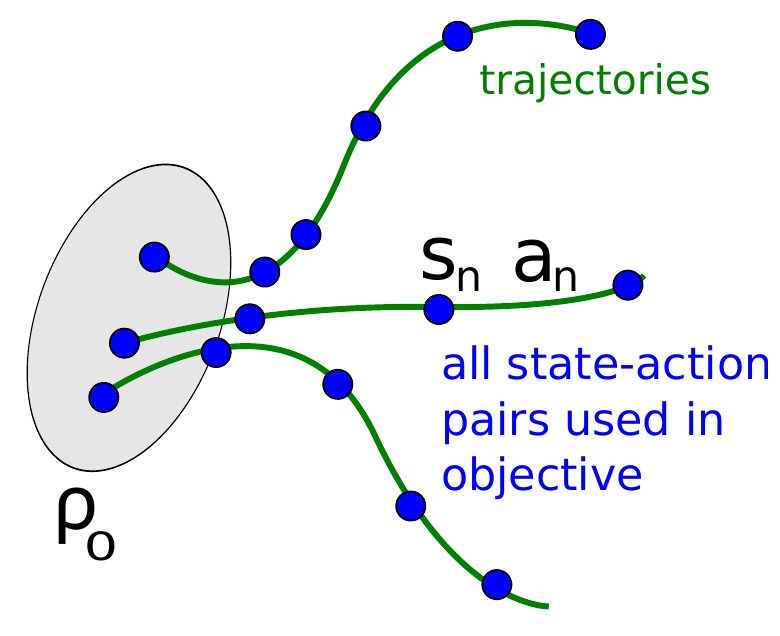
\includegraphics[height=0.32\textheight]{trpo_single_path.png}\par\vspace{6pt}
      \begin{warmbox}
        \centering\small\textbf{\color{AtlasWarm}Single path}
      \end{warmbox}
      \vspace{4pt}
      {\small Roll out $\pi_{\told}$ and use \textbf{every} $(s,a)$ pair encountered along the trajectory.}
    \end{column}
    \begin{column}{0.48\textwidth}
      \centering
      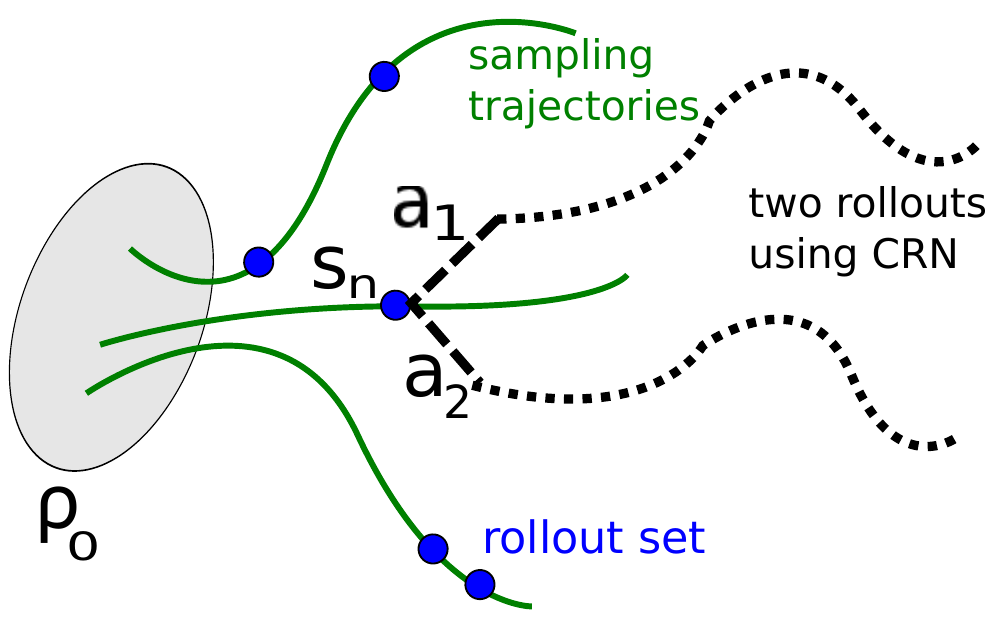
\includegraphics[height=0.32\textheight]{trpo_vine.png}\par\vspace{6pt}
      \begin{coolbox}
        \centering\small\textbf{\color{AtlasCool}Vine}
      \end{coolbox}
      \vspace{4pt}
      {\small From selected states in a trunk rollout, branch out: try multiple actions and run short rollouts.}
    \end{column}
  \end{columns}
  \note{\footnotesize TRPO, Sec.~5.1--5.2, Fig.~1 (figure cropped from the arXiv PDF, p.~4). This slide introduces the two schemes visually; details on the next slide.}
\end{frame}

% ---------------- Single path vs vine - part 2 ----------------
\begin{frame}{Single Path vs Vine: How They Work}
  \begin{columns}[t]
    \begin{column}{0.48\textwidth}
      \begin{warmbox}
        \small\textbf{\color{AtlasWarm}Single path}
        \begin{itemize}\small
          \item Sampling distribution: $q = \pi_{\told}$
          \item $\hat Q$ from discounted return-to-go
          \item Uses \textbf{every} state-action pair
          \item \textbf{No resets needed}
        \end{itemize}
      \end{warmbox}
      \vspace{6pt}
      {\footnotesize\color{AtlasWarm!80!black}\textbf{When:} Real systems, robotics --- anywhere you cannot reset to arbitrary states.}
    \end{column}
    \begin{column}{0.48\textwidth}
      \begin{coolbox}
        \small\textbf{\color{AtlasCool}Vine}
        \begin{itemize}\small
          \item From each state in rollout set: try $K$ actions $a_k\sim q$
          \item Short rollout per action (CRN)
          \item \textbf{Lower variance} $\hat Q$
          \item Needs \textbf{state resets}
        \end{itemize}
      \end{coolbox}
      \vspace{6pt}
      {\footnotesize\color{AtlasCool!80!black}\textbf{When:} Simulators with reset capability --- resets only to states from $\rho_0$ rollouts (not arbitrary $\mu$ like CPI).}
    \end{column}
  \end{columns}
  \vspace{4pt}
  \begin{noteframe}
    \small\textbf{Key limitation both share:} Only actions are reweighted by $\pi_\theta/\pi_{\told}$. States still come from $s\sim\rho_{\told}$ (cannot reweight states without knowing $\rho_\theta/\rho_{\told}$).
  \end{noteframe}
  \note{\footnotesize TRPO, Sec.~5.1--5.2. Single path: uses every $(s_n,a_n)$ from trajectories under $\pi_{\told}$. Vine: from a subset of states (the rollout set), branch into several actions $a_1,a_2$, each followed by a rollout using common random numbers (CRN) to reduce variance. Vine with continuous actions uses self-normalized importance-sampling estimator (removes need for baseline). $q=\pi_{\theta_i}$ for continuous control, uniform for Atari (``can sometimes achieve better exploration''). Vine reset states: ``a subset of $N$ states along these trajectories'' from $s_0\sim\rho_0$ (Sec.~5.2), so unlike CPI's $\mu$ they add no new states. The key limitation (only action reweighting) applies to both and is why TRPO cannot run offline.}
\end{frame}

% ---------------- Solver 1: direction ----------------
\begin{frame}{Solving the Trust-Region Problem: Search Direction}
  \noindent\hfill\trpostep{4}\hfill\null\par\vspace{4pt}
  Approximate around $\told$ --- \textbf{linear} objective, \textbf{quadratic} constraint:
  \begin{gather*}
    L(\theta) \approx L(\told) + g^\top(\theta - \told), \qquad
    \bar D_{\mathrm{KL}}(\told,\theta) \approx \tfrac12(\theta-\told)^\top A\,(\theta-\told)
  \end{gather*}
  \begin{itemize}
    \item $A_{ij} = \frac{\partial^2}{\partial\theta_i\partial\theta_j}\bar D_{\mathrm{KL}}(\told,\theta)$: the \textbf{curvature of the KL}, a.k.a.\ the \textbf{Fisher information matrix}.
    \item Solution direction: $s \propto A^{-1} g$ --- the \textbf{natural gradient}: steepest ascent when distance is measured in KL, not in $\|\theta\|$.
  \end{itemize}
  \simpfooter{$L$ and the KL are nonlinear in $\theta$; an exact constrained solve per batch is too expensive.}
    {First/second-order Taylor models $\Rightarrow$ a closed-form direction $A^{-1}g$.}
    {Valid only locally --- the step must be checked (next slide).}
  \note{\footnotesize TRPO, Sec.~6 and App.~C. $A$ is computed \emph{analytically} as the Hessian of the KL (integrating over actions), not as the covariance of sampled score functions (the ``empirical FIM'' variant in the experiments). With $A^{-1}g$ and a fixed step size we would get exactly Kakade's (2002) natural policy gradient; TRPO instead enforces the constraint at each step. Why the KL has no linear term: it is minimized (zero) at $\theta=\told$, so its gradient vanishes there.}
\end{frame}

% ---------------- Solver 2+3: CG, step size, line search ----------------
\begin{frame}{Computing the Step: Conjugate Gradient + Line Search}
  \noindent\hfill\trpostep{5}\hfill\null\par\vspace{3pt}
  \begin{columns}[T]
    \begin{column}{0.65\textwidth}
      \centering\vspace*{2pt}\small
      \eqstep{1}{\text{Direction: solve $A\,s = g$ by \textbf{conjugate gradient}}\\
        \text{only needs products } y\mapsto Ay \text{ (autodiff), } k=10 \text{ iterations}}
      \eqsep{2}
      \eqstep{2}{\text{Largest step that reaches the KL boundary}\\
        \tfrac12(\beta s)^\top A(\beta s)=\delta \;\Rightarrow\; \beta=\sqrt{2\delta/s^\top A s}}
      \eqsep{3}
      \eqstep{3}{\text{Backtrack } \beta,\ \beta/2,\ \beta/4,\dots \text{ until}\\
        L_{\told}(\theta)\ \text{improves} \ \ \text{and}\ \ \bar D_{\mathrm{KL}}(\told,\theta)\le\delta}
    \end{column}
    \begin{column}{0.02\textwidth}
      {\color{AtlasSlate!40}\vrule width 0.6pt height 0.5\textheight}
    \end{column}
    \begin{column}{0.41\textwidth}
      \centering
      \begin{tikzpicture}[>=Stealth, font=\tiny]
        \path (-2.3,-1.5) rectangle (2.6,1.6);
        \draw[AtlasCool, thick, rotate=25] (0,0) ellipse (2.0 and 0.95);
        \node[text=AtlasCool, anchor=south] at (0.9,1.05) {quadratic model of the KL $=\delta$};
        \uncover<3->{%
          \draw[BadRed, thick, dashed, smooth cycle, tension=0.8]
            plot coordinates {(-1.5,-0.4) (-0.5,-0.8) (0.6,-0.4) (0.7,0.2) (0.2,0.6) (-1.0,0.45)};
          \node[text=BadRed, anchor=north] at (-0.4,-0.9) {true $\bar D_{\mathrm{KL}}\le\delta$};}
        \fill[AtlasInk] (0,0) circle (1.6pt) node[below left]{$\told$};
        \uncover<2->{%
          \draw[->, thick, AtlasSlate] (0,0) -- (25:1.95);
          \fill[AtlasSlate] (25:2.0) circle (1.5pt) node[right]{$\beta s$};}
        \uncover<3->{%
          \fill[BadRed] (25:1.0) circle (1.5pt) node[above left=-1pt]{$\tfrac\beta2$};
          \fill[GoodGreen] (25:0.5) circle (1.8pt) node[below right=-1pt, text=GoodGreen!60!black]{$\tfrac\beta4$ \checkmark};}
      \end{tikzpicture}\par\vspace{2pt}
      \footnotesize
      \only<1>{$A$ has $|\theta|^2$ entries --- never formed.}%
      \only<2>{Step to the edge of the \emph{model}'s trust region.}%
      \only<3->{The model is only local: shrink until the \textbf{true} checks pass.}
    \end{column}
  \end{columns}
  \simpfooter{$A$ cannot even be stored for a neural net; the quadratic model is only local.}
    {CG with Fisher-vector products; full step to $\delta$; line search on the true $L$ and KL.}
    {Second order and \textbf{one step per batch} --- PPO's starting point.}
  \note{\footnotesize TRPO, App.~C and C.1. Conjugate gradient solves $As=g$ with $k$ matrix--vector products and never forms $A$. Fisher-vector product: if the network outputs distribution parameters $\mu_\theta(x)$, then $A=J^\top MJ$ with $J=\partial\mu/\partial\theta$ and $M$ the Fisher matrix of the distribution w.r.t.\ $\mu$ (analytic); $Jy$ and $J^\top v$ are a forward-mode and a backprop pass (the second-derivative term of $\mu$ vanishes at $\theta=\told$). Alternative: generic Hessian-vector products of $\bar D_{\mathrm{KL}}$ --- slightly slower, easier to implement. FVPs on $\sim$10\% of the data, so the total cost is about one gradient. Step size: $s^\top As$ comes for free from CG. Line search objective: $L_{\told}(\theta)-\mathcal X[\bar D_{\mathrm{KL}}\le\delta]$, $\mathcal X=0$ if true, $+\infty$ otherwise; exponential shrinking. Paper: without the line search the algorithm occasionally takes large steps that cause catastrophic drops. Figure (ours, illustrative): the ellipse is $\frac12\Delta^\top A\Delta=\delta$; the dashed region is where the real mean KL is below $\delta$ --- the full step and $\beta/2$ fail, $\beta/4$ is accepted.}
\end{frame}

% ---------------- TRPO algorithm ----------------
\begin{frame}{The TRPO Algorithm}
  \begin{slatebox}
    \textbf{Repeat:}
    \begin{enumerate}
      \item Collect $(s,a)$ pairs with Monte Carlo $\hat Q$ estimates (single path or vine).
      \item Build the sample estimates of the surrogate $L$ and the mean-KL constraint.
      \item Compute $g = \nabla_\theta L$; solve $As = g$ with conjugate gradient (Fisher-vector products).
      \item Step size $\beta = \sqrt{2\delta / s^\top A s}$; backtracking line search on $L$ and the KL.
      \item $\told \leftarrow \told + \beta s$.
    \end{enumerate}
  \end{slatebox}
  \vspace{4pt}
  {\small Cost per update: only slightly more than computing the gradient itself.}
  \note{\footnotesize TRPO, Sec.~6.}
\end{frame}

% ---------------- Recap: chain of approximations ----------------
\begin{frame}[label=trpo-recap]{Recap: From Theory to Practice}
  \begin{center}
  \begin{tikzpicture}[box/.style={draw=AtlasCool, rounded corners, fill=AtlasCool!6, font=\scriptsize, align=center, minimum height=0.9cm, text width=2.6cm},
                      >=Stealth, node distance=0.35cm]
    \node[box] (a) {CPI bound\\(mixtures, $\alpha$)};
    \node[box, right=of a] (b) {Thm.~1\\($\DTV^{\max}$)};
    \node[box, right=of b] (c) {KL penalty\\(MM, monotone)};
    \node[box, right=of c] (d) {Trust region\\($\DKL^{\max}\le\delta$)};
    \node[box, below=0.8cm of d] (e) {Mean KL\\($\bar D_{\mathrm{KL}}\le\delta$)};
    \node[box, left=of e] (f) {Samples + IS\\(single path / vine)};
    \node[box, left=of f] (g) {Linear + quadratic\\(natural gradient)};
    \node[box, left=of g, draw=AtlasWarm, fill=AtlasWarm!8] (h) {CG + line search\\(\textbf{TRPO})};
    \draw[->] (a) -- (b); \draw[->] (b) -- (c); \draw[->] (c) -- (d);
    \draw[->] (d) -- (e); \draw[->] (e) -- (f); \draw[->] (f) -- (g); \draw[->] (g) -- (h);
  \end{tikzpicture}
  \end{center}
  \vspace{4pt}
  \begin{itemize}
    \item First three boxes: \textbf{theory} (monotone improvement). From the trust region on: \textbf{practice} --- each arrow trades a guarantee for practicality.
    \item What's left: noisy $\hat Q$ (GAE) and a heavy second-order solver (PPO). \hfill \hyperlink{trpo-connections}{\beamergotobutton{Related algorithms}}
  \end{itemize}
  \note{\footnotesize Theory ignores advantage-estimation error (Kakade \& Langford handle it; TRPO omits it for simplicity). The backup slide places vanilla PG, natural PG and policy iteration in the same table (TRPO Sec.~7).}
\end{frame}

% % ---------------- What TRPO does not fix: state coverage ----------------
% \begin{frame}[label=trpo-noexplore]{What TRPO Does Not Fix: Where the Data Come From}
%   \begin{columns}[c]
%     \begin{column}{0.50\textwidth}
%       \centering
%       \begin{tikzpicture}[x=0.56cm, y=1cm, font=\footnotesize]
%         \uncover<4->{%
%           \fill[BadRed!8] (6,0) rectangle (10,2.1);
%           \node[font=\scriptsize, BadRed, align=center] at (8,1.7) {no samples:\\no weight can fix this};}
%         % data distribution of the old policy from rho_0
%         \foreach \x/\h in {0/1.6, 1/1.0, 2/0.6, 3/0.32, 4/0.16, 5/0.07, 6/0.025, 7/0.01, 8/0.005, 9/0.002}
%           \fill[AtlasCool!70] (\x+0.12,0) rectangle (\x+0.48,\h);
%         % where a better policy goes
%         \uncover<4->{%
%           \foreach \x/\h in {0/0.3, 1/0.27, 2/0.25, 3/0.23, 4/0.21, 5/0.19, 6/0.17, 7/0.16, 8/0.15, 9/1.1}
%             \fill[AtlasAccent!55] (\x+0.52,0) rectangle (\x+0.88,\h);}
%         % trust region: small change on the visited states
%         \uncover<2->{%
%           \draw[decorate, decoration={brace, amplitude=4pt}, AtlasSlate, thick]
%             (0.1,1.75) -- node[above=4pt, font=\scriptsize, text=AtlasSlate]{trust region acts here} (5.5,1.75);}
%         \draw[gray] (0,0) -- (10,0);
%         \node[below, font=\scriptsize] at (0.5,0) {$s_0$};
%         \node[below, font=\scriptsize] at (9.5,0) {goal};
%         % legend
%         \fill[AtlasCool!70] (0.2,-0.95) rectangle (0.5,-0.75);
%         \node[right, font=\scriptsize] at (0.5,-0.85) {data: $s\sim\rho_{\piold}$ (from $\rho_0$)};
%         \uncover<4->{%
%           \fill[AtlasAccent!55] (6.0,-0.95) rectangle (6.3,-0.75);
%           \node[right, font=\scriptsize] at (6.3,-0.85) {better policy};}
%       \end{tikzpicture}
%     \end{column}
%     \begin{column}{0.48\textwidth}
%       \small
%       \begin{itemize}
%         \item<1-> \textbf{Data:} $s_0\sim\rho_0$, then $\piold$ --- CPI's $\mu$ is gone.
%         \item<2-> \textbf{Trust region:} limits how much $\pi$ changes \textbf{on the states we have}.
%         \item<3-> \textbf{Importance sampling:} reweights \textbf{actions}, never states.
%         \item<3-> \textbf{Vine:} resets only to states already reached from $\rho_0$.
%       \end{itemize}
%     \end{column}
%   \end{columns}

%   \vspace{8pt}
%   \uncover<5->{%
%   \begin{badbox}
%     \small Trust region $\neq$ exploration. Lane \textbf{B} (CPI's Gap~2) stays open in TRPO, GAE and PPO.
%     \hfill \hyperlink{gap2-ex1}{\beamergotobutton{Gap 2, Ex.~1}}
%   \end{badbox}}
%   \note{\footnotesize Our synthesis (it matches the papers' setups). TRPO Sec.~5.1: single path samples $s_0\sim\rho_0$ and simulates $\pi_{\theta_i}$; Sec.~5.2: the vine's rollout set is ``a subset of $N$ states along these trajectories''. Importance sampling (earlier slide): the weight is $\pi_\theta(a\mid s)/\piold(a\mid s)$ at states $s\sim\rho_{\piold}$; reweighting \emph{states} would need $\rho_\theta/\rho_{\piold}$, which is unknown, and for unvisited states there is nothing to reweight. The only exploration left is in the actions: a stochastic policy, a uniform $q$ for the vine on Atari (``can sometimes achieve better exploration'', Sec.~5.2), and later PPO's entropy bonus. Figure: same chain picture as the Gap~2 covariate-shift slide of Part~I. TRPO works well in the experiments because $\rho_0$ and a stochastic policy already cover the relevant states (locomotion from a standing pose, Atari from the start screen).}
% \end{frame}

% ===========================================================================
%  GENERALIZED ADVANTAGE ESTIMATION (Schulman et al., 2015)
% ===========================================================================
\section{Generalized Advantage Estimation}

% Color code (GAE, PPO): warm = value side (critic, advantage estimate),
% cool = policy side, slate = fixed/reference pieces.

% ---------------- Sources: GAE and PPO ----------------
\begin{frame}{GAE and PPO --- Main Sources}
  \begin{center}
    \excalidraw[width=\textwidth, height=0.8\textheight, keepaspectratio]{papers_part2}
  \end{center}
  \note{\footnotesize Practical deep RL on top of TRPO: GAE (Schulman et al., 2015; ICLR 2016) for the advantage estimates, then PPO (Schulman et al., 2017) replacing TRPO's second-order step with a clipped first-order objective. Both papers come from the TRPO group.}
\end{frame}

% ---------------- Bridge: the open problems after TRPO ----------------
\begin{frame}{Where TRPO Leaves Us}
  \centering
  \small
  \begin{tikzpicture}[font=\small, >=Stealth,
      q/.style={rectangle, rounded corners=3pt, line width=0.8pt,
        text width=3.7cm, align=center, inner sep=4pt, minimum height=1.05cm}]
    \node[q, cbox=AtlasSlate, text width=8.2cm] (trpo) at (0,0)
      {\textbf{The TRPO update}\\[2pt]
       $\displaystyle\max_\theta\ \hat\E_t\Big[\frac{\pi_\theta(a_t\mid s_t)}{\pi_{\told}(a_t\mid s_t)}\,
         {\color{AtlasWarm}\hat A_t}\Big]\quad\text{s.t.}\quad
         {\color{AtlasCool}\bar D_{\mathrm{KL}}(\told,\theta)\le\delta}$};
    \node[q, cbox=AtlasWarm] (adv) at (-3.0,-2.0)
      {\textbf{\color{AtlasWarm}Where does $\hat A_t$ come from?}\\ Monte Carlo returns:\\ unbiased, \textbf{high variance}};
    \node[q, cbox=AtlasCool] (sol) at (3.0,-2.0)
      {\textbf{\color{AtlasCool}How is it solved?}\\ CG + line search: second order,\\ \textbf{one step} per batch};
    \draw[->, thick, AtlasWarm] (adv.north) -- (adv.north |- trpo.south);
    \draw[->, thick, AtlasCool] (sol.north) -- (sol.north |- trpo.south);
    \uncover<2->{
      \node[q, cbox=AtlasWarm, fill=AtlasWarm!18!white] (gae) at (-3.0,-4.0)
        {\textbf{GAE} \;{\scriptsize(2015)}\\ a value function trades\\ bias for variance via $\lambda$};
      \node[q, cbox=AtlasCool, fill=AtlasCool!18!white] (ppo) at (3.0,-4.0)
        {\textbf{PPO} \;{\scriptsize(2017)}\\ first order: clip the ratio,\\ $K$ epochs of SGD per batch};
      \draw[->, thick, AtlasWarm] (adv) -- node[right, font=\scriptsize]{fix} (gae);
      \draw[->, thick, AtlasCool] (sol) -- node[right, font=\scriptsize]{fix} (ppo);}
  \end{tikzpicture}
  \note{\footnotesize Our framing. The update is written the way the GAE paper writes TRPO (Sec.~6.1, Eq.~31): ratio times an advantage estimate. TRPO itself used Monte Carlo $\hat Q$ (single path: discounted return-to-go), which differs from an advantage only by a baseline. TRPO, GAE and PPO all sample $s_0\sim\rho_0$ and follow the current policy. PPO's intro lists TRPO's other drawbacks: complicated, and incompatible with noise (dropout) or parameter sharing between policy and value function. GAE was used with TRPO in its own experiments; PPO then uses (truncated) GAE, so the two fixes end up in one algorithm.}
\end{frame}


% ---------------- GAE paper: title + short summary of contribution ----------------
\begin{frame}
  \begin{columns}[c]
    \begin{column}{0.42\textwidth}
      \paperpanel[\large]{High-Dimensional Continuous Control Using Generalized Advantage Estimation}
        {Schulman, Moritz, Levine, Jordan \& Abbeel}{ICLR 2016 (arXiv 2015)}
        {Introduces \textbf{GAE$(\gamma,\lambda)$}: TD($\lambda$) for advantages}
    \end{column}
    \begin{column}{0.55\textwidth}
      \only<1>{%
      {\large\bfseries\color{AtlasAccent}Key Contributions\par}
      \vspace{6pt}
      \small
      \begin{itemize}
        \item \textbf{Solves TRPO's variance problem:} replace Monte Carlo returns with {\color{AtlasWarm}bootstrapped} advantage estimates.
        \item \textbf{Actor--critic architecture:} learn a value function $V_\phi(s)$ alongside the policy.
        \item \textbf{$\lambda$ trades bias for variance:} $\lambda=0$ (pure TD) has low variance, high bias; $\lambda=1$ (Monte Carlo) is unbiased but high variance.
        \item \textbf{GAE$(\gamma,\lambda)$:} exponentially weighted average of $n$-step TD advantages,
          $\hat A_t=\sum_l(\gamma\lambda)^l\delta_{t+l}$, with the \textbf{TD residual}
          {\color{AtlasWarm}$\delta_t = r_t+\gamma V(s_{t+1})-V(s_t)$} (itself a one-step advantage estimate).
      \end{itemize}}%
      \only<2>{%
      % One iteration i of the GAE paper's algorithm (Sec. 6.1): same batch, actor first, critic second.
      {\large\bfseries\color{AtlasAccent}One Iteration: Actor, then Critic\par}
      \vspace{8pt}
      \centering
      \begin{tikzpicture}[font=\scriptsize, >=Stealth,
          st/.style={rectangle, rounded corners=3pt, line width=0.8pt, text width=2.55cm,
            align=center, minimum height=1.15cm, inner sep=3pt}]
        \node[st, cbox=AtlasSlate] (roll) at (0,0)
          {\textbf{1. Rollout}\\ run $\pi_{\theta_i}$ for $N$ steps};
        \node[st, cbox=AtlasWarm] (adv) at (3.4,0)
          {\textbf{\color{AtlasWarm}2. Advantages}\\ $\delta_t$ with the old $V_{\phi_i}$\\ $\hat A_t=\sum_l(\gamma\lambda)^l\delta_{t+l}$};
        \node[st, cbox=AtlasCool] (act) at (3.4,-2.0)
          {\textbf{\color{AtlasCool}3. Actor}\\ TRPO step with $\hat A_t$\\ $\theta_i\to\theta_{i+1}$};
        \node[st, cbox=AtlasWarm, fill=AtlasWarm!18!white] (crit) at (0,-2.0)
          {\textbf{\color{AtlasWarm}4. Critic}\\ fit $V_\phi$ to returns\\ (trust region) $\phi_i\to\phi_{i+1}$};
        \draw[->, thick, AtlasSlate] (roll) -- node[above, font=\tiny]{$s_t,r_t$} (adv);
        \draw[->, thick, AtlasWarm] (adv) -- node[right, font=\tiny]{$\hat A_t$} (act);
        \draw[->, thick, AtlasSlate] (act) -- node[below, font=\tiny, align=center]{same\\batch} (crit);
        \draw[->, thick, AtlasSlate] (crit) -- node[left, font=\tiny]{$i\leftarrow i+1$} (roll);
      \end{tikzpicture}\par\vspace{8pt}
      \raggedright\footnotesize
      \textbf{Order matters:} $\hat A_t$ uses the \emph{old} critic. Fitting $V$ first can overfit the batch $\Rightarrow$ every $\delta_t\approx0$ $\Rightarrow$ zero gradient.}
    \end{column}
  \end{columns}
  \note{\footnotesize Flow: GAE, Sec.~6.1 (algorithm box) and the remark after it: ``the policy update $\theta_i\to\theta_{i+1}$ is performed using the value function $V_{\phi_i}$ for advantage estimation, not $V_{\phi_{i+1}}$. Additional bias would have been introduced if we updated the value function first'' --- in the extreme, an overfit $V$ makes the Bellman residual zero at all timesteps and the gradient estimate zero. The critic step (Sec.~5, Eqs.~28--30) is not TRPO: it is a trust-region regression to Monte Carlo returns, $\min_\phi\sum_n\|V_\phi(s_n)-\hat V_n\|^2$ s.t.\ $\frac1N\sum_n\|V_\phi(s_n)-V_{\phi_{\mathrm{old}}}(s_n)\|^2/(2\sigma^2)\le\epsilon$, i.e.\ a KL trust region for a Gaussian with mean $V_\phi(s)$; solved with CG like TRPO. GAE was used with TRPO here; PPO later adopts (truncated) GAE as its advantage estimator. GAE, Sec.~1--2 and 6. The discounted problem is a special case (absorb $\gamma^t$ into a time-dependent reward). All quantities are unnormalized here, like TRPO and unlike CPI. The formula itself was proposed earlier (Kimura \& Kobayashi 1998; Wawrzy\'nski 2009); the paper's contribution is the analysis that makes it usable with batch trust-region methods, plus the trust-region value-function fit.}
\end{frame}


% % ---------------- GAE paper: title + setting ----------------
% \begin{frame}
%   \begin{columns}[c]
%     \begin{column}{0.42\textwidth}
%       \paperpanel[\large]{High-Dimensional Continuous Control Using Generalized Advantage Estimation}
%         {Schulman, Moritz, Levine, Jordan \& Abbeel}{ICLR 2016 (arXiv 2015)}
%         {Introduces \textbf{GAE$(\gamma,\lambda)$}: TD($\lambda$) for advantages}
%     \end{column}
%     \begin{column}{0.55\textwidth}
%       {\large\bfseries\color{AtlasAccent}Setting \& Assumptions\par}
%       \vspace{6pt}
%       \small
%       \begin{itemize}
%         \item Same MDP as TRPO: start distribution $\rho_0$, unknown dynamics, reward $r_t = r(s_t,a_t,s_{t+1})$.
%         \item \textbf{Undiscounted} goal: maximize $\E\big[\sum_{t} r_t\big]$ (assumed finite).
%         \item $\gamma$ is \textbf{not} part of the problem: an algorithm knob that trades bias for variance.
%         \item Any policy-gradient method --- here TRPO for the policy, a trust region for $V_\phi$ too.
%         \item 3D robots, neural nets with $>10^4$ parameters, torques from raw kinematics.
%       \end{itemize}
%     \end{column}
%   \end{columns}
%   \note{\footnotesize GAE, Sec.~1--2 and 6. The discounted problem is a special case (absorb $\gamma^t$ into a time-dependent reward). All quantities are unnormalized here, like TRPO and unlike CPI. The formula itself was proposed earlier (Kimura \& Kobayashi 1998; Wawrzy\'nski 2009); the paper's contribution is the analysis that makes it usable with batch trust-region methods, plus the trust-region value-function fit.}
% \end{frame}

% % ---------------- What GAE fixes (and what it does not) ----------------
% \begin{frame}{What GAE Fixes --- and What It Does Not}
%   \begin{columns}[c]
%     \begin{column}{0.52\textwidth}
%       \centering
%       \begin{tikzpicture}[x=0.8cm, y=1cm, font=\scriptsize]
%         \path (-5.5,-0.6) rectangle (2.7,2.75);
%         % true value
%         \draw[AtlasInk, dashed] (0,-0.35) -- (0,2.35) node[above, font=\scriptsize]{true $A^\pi(s_t,a_t)$};
%         % rows
%         \foreach \y in {0,0.9,1.8} \draw[gray!60] (-2.6,\y) -- (2.6,\y);
%         \node[anchor=east] at (-2.7,1.8) {$\lambda=1$: returns};
%         \uncover<2->{\node[anchor=east] at (-2.7,0) {$\lambda=0$: one TD step};}
%         \uncover<3->{\node[anchor=east, text=AtlasWarm] at (-2.7,0.9) {$0<\lambda<1$};}
%         % Monte Carlo: centred, wide
%         \foreach \o in {-2.3,-1.6,-1.1,-0.7,-0.3,0.1,0.4,0.9,1.2,1.4,2.0}
%           \fill[AtlasSlate] (\o,1.8) circle (2pt);
%         % TD(0) with an imperfect V: narrow, shifted
%         \uncover<2->{\foreach \o in {-0.25,-0.15,-0.08,0,0.05,0.12,0.2,0.28}
%           \fill[AtlasCool] ({1.1+\o},0) circle (2pt);
%           \draw[<->, BadRed] (0,-0.25) -- node[below, font=\tiny]{bias} (1.1,-0.25);}
%         % in between
%         \uncover<3->{\foreach \o in {-0.9,-0.6,-0.35,-0.1,0.1,0.3,0.55,0.8}
%           \fill[AtlasWarm] ({0.3+\o},0.9) circle (2pt);}
%       \end{tikzpicture}\par
%       {\scriptsize\color{NoteGray} Each dot: one estimate $\hat A_t$ of the same $(s_t,a_t)$ (schematic).}
%     \end{column}
%     \begin{column}{0.46\textwidth}
%       \small
%       \begin{itemize}
%         \item<1-> TRPO multiplies each ratio by $\hat A_t$. From one rollout: \textbf{unbiased}, but \textbf{very noisy}.
%         \item<2-> A learned \textbf{value function} $V$ (the \emph{critic}): low noise, but \textbf{biased} if $V$ is wrong.
%         \item<3-> $\lambda$ slides between the two: a \textbf{bias--variance} knob.
%       \end{itemize}
%     \end{column}
%   \end{columns}

%   \vspace{8pt}
%   \uncover<4->{%
%   \begin{columns}[t]
%     \begin{column}{0.48\textwidth}
%       \begin{goodbox}[equal height group=gaefix]
%         \small\textbf{Fixes:} noisy update directions $\Rightarrow$ fewer samples per step.
%       \end{goodbox}
%     \end{column}
%     \begin{column}{0.48\textwidth}
%       \begin{badbox}[equal height group=gaefix]
%         \small\textbf{Not an exploration knob:} $\lambda$ changes how we \emph{score} sampled actions, not \emph{which states} we visit.
%       \end{badbox}
%     \end{column}
%   \end{columns}}
%   \note{\footnotesize GAE abstract: ``The two main challenges are the large number of samples typically required, and the difficulty of obtaining stable and steady improvement despite the nonstationarity of the incoming data. We address the first challenge by using value functions to substantially reduce the variance of policy gradient estimates at the cost of some bias \ldots\ We address the second challenge by using trust region optimization procedure for both the policy and the value function.'' Sec.~1: actor-critic methods ``use a value function rather than the empirical returns, obtaining an estimator with lower variance at the cost of introducing bias''; and ``bias is more pernicious --- even with an unlimited number of samples, bias can cause the algorithm to fail to converge''. Figure: ours, schematic. Exploration in the GAE setup comes only from the stochastic Gaussian policy; the start distribution is $\rho_0$ as in TRPO (Sec.~2). Next: why the advantage is the right weight, then the estimator itself.}
% \end{frame}

% % ---------------- Which weight multiplies the score? ----------------
% \begin{frame}{Which Weight Multiplies the Score Function?}
%   \begin{columns}[T]
%     \begin{column}{0.5\textwidth}
%       \small
%       \begin{gather*}
%         g = \E\Big[\sum_{t\ge0} \Psi_t\,\nabla_\theta\log\pi_\theta(a_t\mid s_t)\Big]
%       \end{gather*}
%       Same expectation for each choice of $\Psi_t$ --- \textbf{different variance}:\par\vspace{4pt}
%       \renewcommand{\arraystretch}{1.25}
%       \begin{tabular}{r l l}
%         1 & $\sum_{t'\ge0} r_{t'}$ & total return \\
%         2 & $\sum_{t'\ge t} r_{t'}$ & reward after $a_t$ \\
%         3 & $\sum_{t'\ge t} r_{t'} - b(s_t)$ & with a baseline \\
%         4 & $Q^\pi(s_t,a_t)$ & action value \\
%         5 & \alt<2->{\color{AtlasCool}$\boldsymbol{A^\pi(s_t,a_t)}$}{$A^\pi(s_t,a_t)$} & \alt<2->{\color{AtlasCool}\textbf{advantage}}{advantage} \\
%         6 & $r_t + V^\pi(s_{t+1}) - V^\pi(s_t)$ & TD residual
%       \end{tabular}
%     \end{column}
%     \begin{column}{0.02\textwidth}
%       {\color{AtlasSlate!40}\vrule width 0.8pt height 0.66\textheight}
%     \end{column}
%     \begin{column}{0.45\textwidth}
%       \begin{overlayarea}{\linewidth}{0.66\textheight}
%       \centering\footnotesize
%       \uncover<2->{%
%       \begin{tikzpicture}[x=0.78cm, y=0.78cm, >=Stealth]
%         \foreach \x/\q/\p in {1/2.4/0.15, 2/1.76/0.6, 3/0.96/0.45, 4/2.08/0.3} {
%           \fill[AtlasSlate!35] (\x-0.28,1.1) rectangle (\x+0.28,1.1+\q);
%           \fill[AtlasWarm!45] (\x-0.28,0) rectangle (\x+0.28,\p);
%           \node[below] at (\x,0) {$a_\x$};}
%         \draw[gray] (0.4,1.1) -- (4.6,1.1);  \draw[gray] (0.4,0) -- (4.6,0);
%         \node[left] at (0.4,2.5) {$Q^\pi$};
%         \node[left] at (0.4,0.35) {$\pi(a|s)$};
%         \draw[AtlasAccent, very thick, dashed] (0.5,2.75) -- (4.5,2.75) node[right] {$V^\pi$};
%         % push up / down where A > 0 / A < 0
%         \foreach \x/\p in {1/0.15, 2/0.6, 4/0.3}
%           \draw[->, AtlasCool, line width=1.6pt] (\x+0.42,\p) -- ++(0,0.45);
%         \draw[->, AtlasWarm, line width=1.6pt] (3+0.42,0.45) -- ++(0,-0.4);
%       \end{tikzpicture}\par\vspace{4pt}
%       Step along $A\,\nabla\log\pi$: raise $\pi(a|s)$ \textbf{iff} $a$ beats the average $V^\pi$.\par}
%       \vspace{8pt}
%       \uncover<3->{%
%       \begin{slatebox}[top=3pt, bottom=3pt]
%         \small\raggedright\textbf{Discount as a knob:} $A^{\pi,\gamma}$ ignores effects $\gg\frac{1}{1-\gamma}$ steps later $\Rightarrow$ less variance, \textbf{some bias}.
%       \end{slatebox}}
%       \end{overlayarea}
%     \end{column}
%   \end{columns}
%   \note{\footnotesize GAE, Sec.~2, Eq.~1--6. ``The choice $\Psi_t = A^\pi(s_t,a_t)$ yields almost the lowest possible variance'' (Greensmith et al., 2004 for the rigorous version). Intuition from the paper: the gradient term points toward increasing $\pi_\theta(a_t\mid s_t)$ if and only if $A^\pi(s_t,a_t)>0$. Same figure as the Notation slide (step~3): advantages are the gaps to the $V$ line. Step 3: the discounted policy gradient $g^\gamma$ uses $A^{\pi,\gamma}$; an estimator $\hat A_t$ is ``$\gamma$-just'' if it gives an unbiased estimate of $g^\gamma$ (Def.~1, Prop.~1: any unbiased $Q$-estimate minus a baseline that depends only on the past). The paper then only cares about bias \emph{relative to} $g^\gamma$.}
% \end{frame}

% % ---------------- GAE: k-step advantages -> exponential average ----------------
% \begin{frame}{GAE: TD($\lambda$) for Advantages}
%   \begin{columns}[T]
%     \begin{column}{0.53\textwidth}
%       \centering\vspace*{2pt}
%       \small
%       \eqstep{1}{\text{TD residual: one reward, then $V$}\\
%         \delta_t^V = r_t + \gamma V(s_{t+1}) - V(s_t)}
%       \eqsep{2}
%       \eqstep{2}{\text{$k$ residuals: $\hat A_t^{(k)}=\textstyle\sum_{l<k}\gamma^l\delta_{t+l}^V$ telescopes to}\\
%         \hat A_t^{(k)} = -V(s_t) + \textstyle\sum_{l=0}^{k-1}\gamma^l r_{t+l} + \gamma^k V(s_{t+k})}
%       \eqsep{3}
%       \eqstep{3}{\text{all of them: return minus a baseline}\\
%         \hat A_t^{(\infty)} = \textstyle\sum_{l\ge0}\gamma^l r_{t+l} - V(s_t)}
%       \eqsep{4}
%       \eqstep{4}{\text{GAE: average all $k$ with weights $(1-\lambda)\lambda^{k-1}$}\\
%         \hat A_t^{\mathrm{GAE}(\gamma,\lambda)} = \textstyle\sum_{l\ge0}(\gamma\lambda)^l\,\delta_{t+l}^V}
%     \end{column}
%     \begin{column}{0.02\textwidth}
%       {\color{AtlasSlate!40}\vrule width 0.6pt height 0.66\textheight}
%     \end{column}
%     \begin{column}{0.43\textwidth}
%       \centering
%       \begin{tikzpicture}[x=0.76cm, y=0.95cm, >=Stealth,
%           st/.style={circle, fill=AtlasSlate, minimum size=0.16cm, inner sep=0pt},
%           real/.style={AtlasWarm, line width=2.4pt, line cap=round},
%           boot/.style={circle, draw=AtlasWarm, very thick, fill=white, minimum size=0.32cm, inner sep=0pt},
%           base/.style={rectangle, draw=AtlasSlate, thick, fill=AtlasSlate!25, minimum size=0.22cm, inner sep=0pt},
%           lab/.style={font=\scriptsize, anchor=east}]
%         \foreach \i/\n in {0/t, 1/t{+}1, 2/t{+}2, 3/t{+}3, 4/t{+}4}
%           \node[st] (s\i) at (\i,0) {};
%         \foreach \i/\n in {0/t, 1/t{+}1, 2/t{+}2, 3/t{+}3, 4/t{+}4}
%           \node[font=\tiny, above=2pt of s\i] {$s_{\n}$};
%         \foreach \i/\j/\r in {0/1/t, 1/2/t{+}1, 2/3/t{+}2, 3/4/t{+}3}
%           \draw[->, AtlasSlate, shorten <=2pt, shorten >=2pt] (s\i) -- node[below=1pt, font=\tiny]{$r_{\r}$} (s\j);
%         \draw[->, AtlasSlate, shorten <=2pt] (s4) -- (5.0,0) node[right, font=\scriptsize]{$\cdots$};
%         % k = 1
%         \uncover<1->{
%           \node[lab] at (-0.3,-1.0) {$k=1$};
%           \draw[real] (0,-1.0) -- (1,-1.0);
%           \node[base] at (0,-1.0) {};
%           \node[boot] at (1,-1.0) {};}
%         % k = 3
%         \uncover<2->{
%           \node[lab] at (-0.3,-1.7) {$k=3$};
%           \draw[real] (0,-1.7) -- (3,-1.7);
%           \node[base] at (0,-1.7) {};
%           \node[boot] at (3,-1.7) {};}
%         % k = infinity
%         \uncover<3->{
%           \node[lab] at (-0.3,-2.4) {$k=\infty$};
%           \draw[real] (0,-2.4) -- (5.3,-2.4);
%           \node[base] at (0,-2.4) {};
%           \draw[AtlasWarm, thick] (5.3,-2.55) -- (5.3,-2.25);}
%         % legend
%         \node[font=\tiny, anchor=west] at (-1.1,-3.05)
%           {\tikz\node[base]{}; $-V(s_t)$ \;\;
%            \tikz\draw[real] (0,0) -- (0.35,0); rewards \;\;
%            \tikz\node[boot] {}; $\gamma^kV(s_{t+k})$};
%         % spectrum
%         \uncover<4->{
%           \draw[<->, thick, AtlasSlate] (0,-3.75) -- (5.3,-3.75);
%           \node[font=\scriptsize, below] at (0,-3.8) {$\lambda=0$};
%           \node[font=\scriptsize, below] at (5.3,-3.8) {$\lambda=1$};
%           \node[font=\tiny, align=center, below] at (1.0,-4.25) {low variance\\biased unless $V=V^{\pi,\gamma}$};
%           \node[font=\tiny, align=center, below] at (4.3,-4.25) {unbiased for $g^\gamma$, any $V$\\high variance};}
%       \end{tikzpicture}
%     \end{column}
%   \end{columns}
%   \note{\footnotesize GAE, Sec.~3, Eqs.~10--18. Same picture as our TD(0)$\to$MC slide in Part~I: TD($\lambda$) estimates a value, GAE estimates an advantage; the only change is the baseline $-V(s_t)$ at the start of every row. $\delta^V_t$ is an unbiased advantage estimate only if $V = V^{\pi,\gamma}$. The bias shrinks as $k$ grows because the bootstrapped term $\gamma^kV(s_{t+k})$ is discounted more, while $-V(s_t)$ never adds bias (it is a baseline). The geometric weights $(1-\lambda)\lambda^{k-1}$ sum to~1, and the sum collapses to a $(\gamma\lambda)$-discounted sum of TD residuals (Eq.~16). Unnormalized, like TRPO.}
% \end{frame}

% % ---------------- Two knobs: gamma and lambda ----------------
% \begin{frame}{Two Knobs, Two Kinds of Bias}
%   \begin{columns}[c]
%     \begin{column}{0.5\textwidth}
%       \centering
%       \begin{tikzpicture}[x=0.9cm, y=1.6cm, >=Stealth,
%           declare function={raw(\x) = 0.25 + 0.55*exp(-0.18*\x) + 0.12*sin(deg(1.3*\x))*exp(-0.08*\x);
%                              shaped(\x) = 1.1*exp(-1.3*\x);}]
%         \draw[->, gray] (0,0) -- (6.3,0) node[right, font=\scriptsize]{$l$};
%         \draw[->, gray] (0,0) -- (0,1.35) node[left, font=\scriptsize]{$|\chi|$};
%         % windows first, curves on top
%         \fill[AtlasSlate!10] (0,0) rectangle (4.6,1.2);
%         \uncover<2->{\fill[AtlasWarm!18] (0,0) rectangle (1.8,1.2);}
%         \draw[dashed, AtlasSlate] (4.6,0) node[below, font=\scriptsize]{$\frac{1}{1-\gamma}$} -- (4.6,1.2);
%         \draw[AtlasSlate, very thick, domain=0:6.1, samples=80, smooth] plot (\x, {raw(\x)});
%         \node[AtlasSlate, font=\scriptsize] at (5.45,0.85) {raw reward};
%         \uncover<2->{
%           \draw[dashed, AtlasWarm] (1.8,0) node[below, font=\scriptsize]{$\frac{1}{1-\gamma\lambda}$} -- (1.8,1.2);
%           \draw[AtlasWarm, very thick, domain=0:6.1, samples=60, smooth] plot (\x, {shaped(\x)});
%           \node[AtlasWarm, font=\scriptsize, anchor=west] at (1.9,1.05) {shaped by $V$: $\delta^V$};}
%       \end{tikzpicture}\par\vspace{4pt}
%       {\scriptsize\color{NoteGray}$\chi(l;s,a)=\E[r_{t+l}\mid s,a]-\E[r_{t+l}\mid s]$: how long $a_t$ keeps mattering}
%     \end{column}
%     \begin{column}{0.48\textwidth}
%       \small
%       \textbf{\color{AtlasSlate}$\gamma$: cut the horizon}\\
%       Drops effects after $\approx\frac{1}{1-\gamma}$ steps. \\
%       Biased \textbf{even with the exact} $V$.

%       \vspace{8pt}
%       \uncover<2->{
%         \textbf{\color{AtlasWarm}$\lambda$: shape, then cut again}\\
%         $\delta^V$ is the reward shaped by $\Phi = V$: a good $V$ pulls the effect of $a_t$ to $l\approx0$. \\
%         Biased \textbf{only if $V$ is wrong}.}

%       \vspace{8pt}
%       \uncover<3->{
%       \begin{slatebox}[top=3pt, bottom=3pt]
%         \small So the best $\lambda$ is \textbf{lower} than the best $\gamma$ (numbers at the end).
%       \end{slatebox}}
%     \end{column}
%   \end{columns}
%   \note{\footnotesize GAE, Sec.~3 (end) and Sec.~4. $\gamma$ sets the scale of $V^{\pi,\gamma}$ and adds bias regardless of the value function's accuracy; $\lambda<1$ adds bias only when $V$ is inaccurate --- hence the best $\lambda$ is much lower than the best $\gamma$. Reward shaping (Ng et al., 1999): $\tilde r = r + \gamma\Phi(s') - \Phi(s)$ leaves $A^{\pi,\gamma}$ unchanged; with $\Phi = V$ it is exactly $\delta^V$, and GAE is the $(\gamma\lambda)$-discounted sum of shaped rewards (Eq.~20). With $\Phi = V^{\pi,\gamma}$ the response of the shaped reward is nonzero only at $l=0$. Response function: Eq.~22, $A^{\pi,\gamma}(s,a)=\sum_l\gamma^l\chi(l;s,a)$. Curves are illustrative. Numbers: Sec.~6.3 (cart-pole: $\gamma\in[0.96,0.99]$, $\lambda\in[0.92,0.99]$); Discussion: $\lambda\in[0.9,0.99]$ ``usually'' best; App.~A.2: the $\lambda=0$ estimator was ``prohibitively'' biased.}
% \end{frame}

% % ---------------- GAE + TRPO: actor and critic ----------------
% \begin{frame}{Actor--Critic: Policy and Value Networks}
%   \begin{columns}[T]
%     \begin{column}{0.52\textwidth}
%       \centering
%       \begin{tikzpicture}[font=\scriptsize, >=Stealth,
%           ac/.style={rectangle, rounded corners=3pt, line width=0.8pt, text width=2.7cm,
%             align=center, minimum height=0.9cm, inner sep=3pt}]
%         \node[ac, cbox=AtlasSlate] (env) at (0,0) {\textbf{1. Rollouts}\\ run $\pi_{\theta_i}$ for $N$ steps};
%         \uncover<2->{%
%           \node[ac, cbox=AtlasWarm] (crit) at (1.85,-1.85)
%             {\textbf{\color{AtlasWarm}2. Critic $V_{\phi_i}$}\\ $\delta_t^V$, \ $\hat A_t=\sum_l(\gamma\lambda)^l\delta_{t+l}^V$};
%           \draw[->, thick, AtlasSlate] (env) -- node[right, font=\tiny]{$s_t, r_t$} (crit);}
%         \uncover<3->{%
%           \node[ac, cbox=AtlasCool] (act) at (-1.85,-1.85)
%             {\textbf{\color{AtlasCool}3. Actor $\pi_\theta$}\\ TRPO step with $\hat A_t$};
%           \draw[->, thick, AtlasWarm] (crit) -- node[above, font=\tiny]{$\hat A_t$} (act);
%           \draw[->, thick, AtlasCool] (act) -- node[left, font=\tiny]{$\theta_{i+1}$} (env);}
%         \uncover<4->{%
%           \node[ac, cbox=AtlasWarm, fill=AtlasWarm!18!white] (fit) at (1.85,-3.55)
%             {\textbf{4. Fit the critic}\\ regression, trust region $\to\phi_{i+1}$};
%           \draw[->, thick, AtlasWarm] (crit) -- node[right, font=\tiny]{after 3} (fit);}
%       \end{tikzpicture}\par\vspace{4pt}
%       \uncover<4->{{\scriptsize\color{NoteGray} Order matters: fit $V$ \emph{after} computing $\hat A_t$ --- an overfit $V$ makes every $\delta_t^V=0$.}}
%     \end{column}
%     \begin{column}{0.46\textwidth}
%       \small
%       \begin{itemize}
%         \item \textbf{Actor}: the policy network, updated by TRPO.
%         \item \textbf{Critic}: a second network $V_\phi(s)\approx V^{\pi,\gamma}(s)$, fitted by regression to returns.
%       \end{itemize}
%       \uncover<4->{%
%       {\color{AtlasWarm}\textbf{Value fit with a trust region}}
%       \begin{warmformulabox}
%         \begin{gather*}
%           \min_\phi\ \sum_n \big\|V_\phi(s_n) - \hat V_n\big\|^2 \\
%           \text{s.t.}\ \ \frac1N\sum_n \frac{\|V_\phi(s_n) - V_{\phi_{\mathrm{old}}}(s_n)\|^2}{2\sigma^2} \le \epsilon
%         \end{gather*}
%       \end{warmformulabox}
%       {\footnotesize $=$ a KL trust region for a Gaussian with mean $V_\phi(s)$; solved with CG, like TRPO.}}
%     \end{column}
%   \end{columns}
%   \note{\footnotesize GAE, Sec.~5 (Eqs.~28--30) and Sec.~6.1 (algorithm). Actor-critic: the ``actor'' is the policy, the ``critic'' is the learned value function that scores its actions (Konda \& Tsitsiklis 2003, cited in GAE Sec.~1). Unlike Q-learning-style critics (e.g.\ SAC, which learns $Q(s,a)$ off-policy), GAE's critic is a state-value $V(s)$ fitted on-policy to Monte Carlo returns $\hat V_n=\sum_l\gamma^l r_{n+l}$ (TD($\lambda$) targets gave no difference). $\sigma^2$ is the current mean squared error. The trust region keeps $V$ from overfitting the latest batch --- the second challenge of the abstract (stable improvement). Networks: three hidden layers (100, 50, 25 tanh units) for both policy and value. Results (3D biped etc.) are on the Experiments slides at the end.}
% \end{frame}

% ===========================================================================
%  PROXIMAL POLICY OPTIMIZATION (Schulman et al., 2017)
% ===========================================================================
\section{Proximal Policy Optimization}

% ---------------- PPO paper: title + setting ----------------
\begin{frame}
  \begin{columns}[c]
    \begin{column}{0.4\textwidth}
      \paperpanel{Proximal Policy Optimization Algorithms}
        {Schulman, Wolski, Dhariwal, Radford \& Klimov}{arXiv 2017 (OpenAI)}
        {Introduces \textbf{PPO}: TRPO's reliability with only \textbf{first-order} SGD}
    \end{column}
    \begin{column}{0.57\textwidth}
      {\large\bfseries\color{AtlasAccent}Setting \& Motivation\par}
      \vspace{6pt}
      \small
      \begin{itemize}
        \item Same setting as TRPO; advantages $\hat A_t$ from (truncated) \textbf{GAE}.
        \item \textbf{TRPO}: complicated; no dropout, no parameter sharing between policy and value.
        \item \textbf{Vanilla PG}: several steps on the same batch $\Rightarrow$ destructively large updates.
        \item \textbf{Goal}: reuse each batch for many SGD steps, without leaving the trust region.
        \item Tested on MuJoCo and 49 Atari games.
      \end{itemize}
    \end{column}
  \end{columns}
  \note{\footnotesize PPO, Sec.~1--2. ``Vanilla'' PG estimator: $\hat g=\hat\E_t[\nabla_\theta\log\pi_\theta(a_t\mid s_t)\hat A_t]$, from the loss $L^{PG}=\hat\E_t[\log\pi_\theta\,\hat A_t]$; multiple optimization steps on $L^{PG}$ are ``not well-justified''. $\hat\E_t$ is the empirical average over a batch. Q-learning with function approximation is also dismissed: fails on many simple problems, and no strong continuous-control results at the time.}
\end{frame}

% ---------------- PPO's goal: many SGD steps per batch ----------------
\begin{frame}{PPO's Goal: Many SGD Steps per Batch}
  \begin{columns}[T]
    \begin{column}{0.52\textwidth}
      \centering
      \begin{tikzpicture}[x=0.55cm, y=1cm, font=\tiny]
        % TRPO row: collect -> one step -> collect ...
        \node[font=\scriptsize\bfseries, anchor=east] at (-0.2,1.3) {TRPO};
        \foreach \a/\b in {0/3, 3.4/6.4, 6.8/9.8} {
          \fill[AtlasSlate!15] (\a,1.1) rectangle (\b,1.5);
          \node at ({(\a+\b)/2},1.3) {collect};}
        \foreach \a in {3, 6.4, 9.8}
          \fill[AtlasCool] (\a,1.1) rectangle (\a+0.4,1.5);
        % PPO row: collect -> K epochs -> collect ...
        \uncover<2->{%
          \node[font=\scriptsize\bfseries, anchor=east, text=AtlasCool] at (-0.2,0.3) {PPO};
          \foreach \a/\b in {0/3, 5.4/8.4} {
            \fill[AtlasSlate!15] (\a,0.1) rectangle (\b,0.5);
            \node at ({(\a+\b)/2},0.3) {collect};}
          \foreach \a in {3, 3.6, 4.2, 4.8, 8.4, 9.0, 9.6}
            \fill[AtlasCool!60] (\a+0.04,0.1) rectangle (\a+0.56,0.5);
          \draw[decorate, decoration={brace, mirror, amplitude=3pt}, AtlasCool]
            (3,0.0) -- node[below=3pt, text=AtlasCool]{$K$ epochs, minibatches} (5.4,0.0);}
        \draw[->, gray] (0,-0.65) -- (10.4,-0.65) node[right]{time};
        % legend
        \fill[AtlasCool] (0,1.85) rectangle (0.4,2.05);
        \node[anchor=west] at (0.45,1.95) {policy update};
        \fill[AtlasSlate!15] (4.2,1.85) rectangle (4.6,2.05);
        \node[anchor=west] at (4.65,1.95) {environment samples};
      \end{tikzpicture}\par\vspace{6pt}
      \footnotesize
      \only<1>{TRPO: one (expensive) step, then the batch is thrown away.}%
      \only<2->{PPO: squeeze the same batch with cheap first-order steps.}
    \end{column}
    \begin{column}{0.02\textwidth}
      {\color{AtlasSlate!40}\vrule width 0.6pt height 0.55\textheight}
    \end{column}
    \begin{column}{0.44\textwidth}
      \centering
      \uncover<3->{%
      \begin{tikzpicture}[x=1.05cm, y=0.5cm, >=Stealth, font=\scriptsize]
        \fill[GoodGreen!15] (0,0.8) rectangle (4.3,1.2);
        \node[font=\tiny, text=GoodGreen!60!black, anchor=west] at (2.0,0.45) {data trustworthy: $r_t\approx1$};
        \draw[->, gray] (0,0) -- (4.4,0) node[right]{epoch};
        \draw[->, gray] (0,0) -- (0,5.6) node[above]{$r_t=\frac{\pi_\theta(a_t|s_t)}{\piold(a_t|s_t)}$};
        \foreach \k in {0,...,4} \draw (\k,0) -- (\k,-0.12) node[below, font=\tiny]{\k};
        \draw[AtlasCool, very thick] (0,1) -- (1,1.2) -- (2,1.5) -- (3,2) -- (4,5);
        \foreach \k/\r in {0/1, 1/1.2, 2/1.5, 3/2, 4/5} \fill[AtlasCool] (\k,\r) circle (2pt);
        \node[font=\tiny, anchor=east] at (3.9,5.0) {$\hat A_t>0$: $L^{CPI}$ term $r_t\hat A_t$ still rising};
      \end{tikzpicture}\par\vspace{2pt}
      {\footnotesize One sample, $\hat A_t>0$: \textbf{nothing says stop}.}}
    \end{column}
  \end{columns}

  \vspace{6pt}
  \uncover<4->{%
  \begin{badbox}
    \small The data came from $\piold$: the surrogate is trustworthy only near $r_t=1$. Unchecked, repeated steps give \textbf{destructively large} updates.
  \end{badbox}}
  \note{\footnotesize PPO, abstract and Sec.~2: ``standard policy gradient methods perform one gradient update per data sample''; PPO ``enables multiple epochs of minibatch updates''. On the vanilla loss: ``While it is appealing to perform multiple steps of optimization on this loss using the same trajectory, doing so is not well-justified, and empirically it often leads to destructively large policy updates.'' TRPO also takes one step per batch (a large, carefully constrained one). Right plot: ours, illustrative --- the per-sample term $r_t\hat A_t$ of the CPI/TRPO surrogate is linear in $r_t$, so for $\hat A_t>0$ gradient ascent keeps pushing $\pi_\theta(a_t\mid s_t)$ up for as long as we keep optimizing; only TRPO's KL constraint stopped it. PPO's question: how to stop it with an ordinary first-order optimizer.}
\end{frame}

% ---------------- From the CPI surrogate to a first-order objective ----------------
\begin{frame}{Back to the CPI Surrogate}
  \noindent{\small Ratio $=$ TRPO's importance weight:\quad
    $r_t(\theta) = \dfrac{\pi_\theta(a_t\mid s_t)}{\pi_{\told}(a_t\mid s_t)}$,\quad $r_t(\told)=1$}
  \begin{formulabox}
    \begin{gather*}
      L^{CPI}(\theta) = \hat\E_t\big[r_t(\theta)\,\hat A_t\big]
      \qquad\text{\small (``CPI'': Kakade \& Langford)}
    \end{gather*}
  \end{formulabox}
  \uncover<2->{%
  \begin{badbox}
    \small Many SGD steps on $L^{CPI}$ alone: $r_t$ runs far from 1 $\Rightarrow$ huge updates. Score $-0.39$: worse than random.
  \end{badbox}}
  \vspace{2pt}
  \uncover<3->{%
  \begin{columns}[t]
    \begin{column}{0.32\textwidth}
      \begin{slatebox}[equal height group=ppoopts]
        \small\textbf{Constraint} (TRPO)\\[2pt]
        s.t.\ $\hat\E_t[\DKL]\le\delta$\\[2pt]
        {\scriptsize second-order solver}
      \end{slatebox}
    \end{column}
    \begin{column}{0.32\textwidth}
      \begin{warmbox}[equal height group=ppoopts]
        \small\textbf{\color{AtlasWarm}Penalty} (baseline)\\[2pt]
        $-\beta\,\hat\E_t[\DKL]$\\[2pt]
        {\scriptsize no single $\beta$ works $\to$ adapt it}
      \end{warmbox}
    \end{column}
    \begin{column}{0.32\textwidth}
      \begin{coolbox}[equal height group=ppoopts]
        \small\textbf{\color{AtlasCool}Clip} (``PPO'')\\[2pt]
        no gain once $|r_t-1|>\epsilon$\\[2pt]
        {\scriptsize first order, next slide}
      \end{coolbox}
    \end{column}
  \end{columns}}
  \note{\footnotesize PPO, Sec.~2.2--3, Eq.~6: ``The superscript CPI refers to conservative policy iteration [KL02], where this objective was proposed.'' It is TRPO's $L_{\told}$ written with sample averages; its gradient at $\told$ equals the vanilla policy gradient. The penalty form is what TRPO's theory suggests (the KL bound with constant $C$); TRPO used a constraint because ``it is hard to choose a single value of $\beta$ that performs well across different problems --- or even within a single problem''. Score $-0.39$: Table~1, ``no clipping or penalty'' (normalized so random $=0$, best $=1$; HalfCheetah went very negative).}
\end{frame}

% ---------------- The clipped surrogate ----------------
\begin{frame}{The Clipped Surrogate Objective}
  \begin{formulabox}
    \begin{gather*}
      L^{CLIP}(\theta) = \hat\E_t\Big[\min\big(r_t(\theta)\hat A_t,\ \mathrm{clip}(r_t(\theta),1-\epsilon,1+\epsilon)\,\hat A_t\big)\Big],
      \qquad \epsilon = 0.2
    \end{gather*}
  \end{formulabox}
  \vspace{2pt}
  \begin{columns}[T]
    \begin{column}{0.48\textwidth}
      \centering
      \begin{tikzpicture}[x=2.0cm, y=1.05cm, >=Stealth]
        \node[font=\small] at (1.0,1.95) {$\hat A_t > 0$};
        \draw[->, gray] (0,0) -- (2.15,0) node[right, font=\scriptsize]{$r$};
        \draw[->, gray] (0,-0.1) -- (0,1.7);
        \uncover<3->{\draw[dashed, gray, thick] (1.2,1.2) -- (1.65,1.65) node[right, font=\tiny]{$L^{CPI}$};}
        \draw[AtlasCool, very thick] (0,0) -- (1.2,1.2) -- (2.05,1.2);
        \draw[dotted, gray] (1.2,0) node[below right=-1pt, font=\tiny]{$1{+}\epsilon$} -- (1.2,1.2);
        \draw[dotted, gray] (1,0) node[below left=-1pt, font=\tiny]{$1$} -- (1,1);
        \fill[BadRed] (1,1) circle (2pt);
      \end{tikzpicture}\par
      {\scriptsize Raise $\pi(a_t|s_t)$ --- no extra gain past $1+\epsilon$.\par}
      \uncover<4->{{\scriptsize\color{BadRed} Wrong way ($r<1-\epsilon$): not clipped, objective keeps falling.\par}}
    \end{column}
    \begin{column}{0.48\textwidth}
      \centering
      \uncover<2->{%
      \begin{tikzpicture}[x=2.0cm, y=1.05cm, >=Stealth]
        \node[font=\small] at (1.0,0.75) {$\hat A_t < 0$};
        \draw[->, gray] (0,0) -- (2.15,0) node[right, font=\scriptsize]{$r$};
        \draw[->, gray] (0,0.1) -- (0,-2.1);
        \uncover<3->{\draw[dashed, gray, thick] (0,0) -- (0.8,-0.8) node[pos=0.45, above right, font=\tiny]{$L^{CPI}$};}
        \draw[AtlasWarm, very thick] (0,-0.8) -- (0.8,-0.8) -- (2.05,-2.05);
        \draw[dotted, gray] (0.8,0) node[above left=-1pt, font=\tiny]{$1{-}\epsilon$} -- (0.8,-0.8);
        \draw[dotted, gray] (1,0) node[above right=-1pt, font=\tiny]{$1$} -- (1,-1);
        \fill[BadRed] (1,-1) circle (2pt);
      \end{tikzpicture}\par
      {\scriptsize Lower $\pi(a_t|s_t)$ --- no extra gain below $1-\epsilon$.\par}
      \uncover<4->{{\scriptsize\color{BadRed} Wrong way ($r>1+\epsilon$): not clipped, objective keeps falling.\par}}}
    \end{column}
  \end{columns}
  \vspace{4pt}
  \uncover<3->{\centering\small $\min$ $\Rightarrow$ $L^{CLIP}\le L^{CPI}$: clipping removes \textbf{gains}, never hides \textbf{drops} --- a pessimistic bound.\par}
  \uncover<4->{\centering\small Moving the wrong way keeps its gradient: the update can always pull $r_t$ \textbf{back} toward 1.\par}
  \note{\footnotesize PPO, Sec.~3, Eq.~7 and Fig.~1 (redrawn; red dot $=$ start of the optimization, $r=1$). One term of the sum is shown. The gradient of a clipped term is zero only when the ratio is outside the interval \emph{in the direction that would improve} the objective; in the other direction the unclipped term is active and the update can still pull the ratio back. $L^{CLIP}=L^{CPI}$ to first order at $\told$. Fig.~2 of the paper: along the update direction, $L^{CLIP}$ peaks at a KL of about 0.02 (Hopper). Our remark, not the paper's: clipping does not strictly bound the KL --- states whose terms are clipped can still move through shared parameters.}
\end{frame}

% ---------------- What clipping replaces ----------------
\begin{frame}{What Clipping Replaces}
  \centering
  \begin{tikzpicture}[font=\footnotesize, >=Stealth,
      cr/.style={rectangle, rounded corners=3pt, line width=0.8pt, text width=3.5cm,
        align=center, minimum height=1.9cm, inner sep=4pt}]
    \node[cr, cbox=AtlasWarm] (c) at (0,0)
      {\textbf{\color{AtlasWarm}CPI}\\[2pt] mixture step\\ $\pinew=(1-\alpha)\pi+\alpha\pi'$\\[2pt] {\scriptsize close \textbf{by construction}}};
    \uncover<2->{%
      \node[cr, cbox=AtlasSlate] (t) at (5.0,0)
        {\textbf{TRPO}\\[2pt] KL constraint\\ $\bar D_{\mathrm{KL}}(\told,\theta)\le\delta$\\[2pt] {\scriptsize close \textbf{by a solver} (2nd order)}};
      \draw[->, thick, AtlasSlate] (c) -- node[above, font=\scriptsize]{any $\pi_\theta$} (t);}
    \uncover<3->{%
      \node[cr, cbox=AtlasCool] (p) at (10.2,0)
        {\textbf{\color{AtlasCool}PPO}\\[2pt] clipped ratio\\ $r_t\in[1-\epsilon,1+\epsilon]$\\[2pt] {\scriptsize close \textbf{by the objective} (1st order)}};
      \draw[->, thick, AtlasCool] (t) -- node[above, font=\scriptsize]{first order} (p);}
  \end{tikzpicture}

  \vspace{12pt}
  \raggedright
  \uncover<3->{\small \textbf{Proximal}: keep $\pi_\theta$ near $\piold$ --- with plain minibatch SGD/Adam, several epochs per batch.\par}
  \vspace{8pt}
  \uncover<4->{%
  \begin{badbox}
    \small Clipping removes the \textbf{incentive} to move a ratio further --- it does not \textbf{enforce} a limit. No KL bound is guaranteed.
  \end{badbox}}
  \note{\footnotesize Our summary. CPI: the new policy differs from the old one with probability at most $\alpha$ per state, by construction of the mixture, with $\alpha$ from Cor.~4.2. TRPO: any $\pi_\theta$, distance measured by the mean KL, enforced by CG + line search. PPO: the constraint disappears from the optimizer and becomes a property of the objective; once $r_t$ leaves $[1-\epsilon,1+\epsilon]$ in the improving direction its gradient is zero. Caveat (our remark, studied later, e.g.\ Engstrom et al., 2020, ``Implementation Matters in Deep Policy Gradients''): the gradient of the other, unclipped samples still moves shared parameters, so clipped samples can keep drifting and the KL is not bounded; in practice it stays small (PPO Fig.~2: about 0.02 at the maximum of $L^{CLIP}$ on Hopper). Some implementations add early stopping on the KL for this reason.}
\end{frame}

% ---------------- PPO algorithm ----------------
\begin{frame}{PPO in Practice}
  \begin{formulabox}
    \begin{gather*}
      L_t^{CLIP+VF+S}(\theta) = \hat\E_t\Big[\underbrace{L_t^{CLIP}(\theta)}_{\text{policy}}
        - c_1\underbrace{\big(V_\theta(s_t)-V_t^{\mathrm{targ}}\big)^2}_{\text{\color{AtlasWarm}value}}
        + c_2\underbrace{S[\pi_\theta](s_t)}_{\text{entropy}}\Big]
    \end{gather*}
  \end{formulabox}
  \begin{columns}[T]
    \begin{column}{0.55\textwidth}
      \begin{slatebox}
        \small\textbf{Each iteration:}
        \begin{enumerate}
          \item $N$ actors run $\pi_{\told}$ for $T$ steps each.
          \item Truncated GAE: $\hat A_t = \sum_{l=0}^{T-t-1}(\gamma\lambda)^l\delta_{t+l}$.
          \item $K$ epochs of minibatch Adam on $L$.
          \item $\told\leftarrow\theta$.
        \end{enumerate}
      \end{slatebox}
    \end{column}
    \begin{column}{0.42\textwidth}
      \begin{coolbox}
        \small\textbf{\color{AtlasCool}The point:} $K$ epochs on the \textbf{same} batch.\\[2pt]
        TRPO took \textbf{one} step per batch; clipping is what makes reuse safe.
      \end{coolbox}
      \vspace{4pt}
      {\scriptsize $\delta_t = r_t+\gamma V(s_{t+1})-V(s_t)$: TD residual, as in GAE.\par}
    \end{column}
  \end{columns}
  \note{\footnotesize PPO, Sec.~5 (Eqs.~9--12, Alg.~1) and Table~3. MuJoCo settings (Table~3): $T=2048$, $K=10$ epochs, minibatch 64, $\gamma=0.99$, $\lambda=0.95$, $\epsilon=0.2$. Abstract: ``we propose a novel objective function that enables multiple epochs of minibatch updates''. $c_1$ only matters when policy and value share parameters; the entropy bonus $S$ encourages exploration (Williams 1992; Mnih et al.\ 2016). Truncated GAE does not look beyond the segment end $T$, which suits fixed-length segments and recurrent nets. Atari settings (Table~5): $T=128$, 3 epochs, 8 actors, $\epsilon=0.1\alpha$ with $\alpha$ annealed $1\to0$, $c_1=1$, $c_2=0.01$. The entropy bonus is PPO's only explicit exploration term (``to ensure sufficient exploration'', Sec.~5) --- it acts on the action distribution, not on where episodes start. Results: Experiments section at the end.}
\end{frame}

% ---------------- TRPO vs PPO ----------------
\begin{frame}{TRPO vs.\ PPO}
  \begin{center}
  \renewcommand{\arraystretch}{1.3}
  \small
  \begin{tabular}{l l l}
    \toprule
     & \textbf{TRPO} & \textbf{\color{AtlasCool}PPO} \\
    \midrule
    Stay close by & KL constraint $\bar D_{\mathrm{KL}}\le\delta$ & clipped ratio $[1-\epsilon,1+\epsilon]$ \\
    Solver & CG + line search (2nd order) & minibatch Adam (1st order) \\
    Steps per batch & one & $K$ epochs \\
    Policy + value & separate networks & may share (one loss) \\
    Advantages & Monte Carlo $\hat Q$ & truncated GAE \\
    States from & $s_0\sim\rho_0$, then $\piold$ & same --- still no $\mu$ \\
    \bottomrule
  \end{tabular}
  \end{center}
  \vspace{2pt}
  \begin{columns}[t]
    \begin{column}{0.48\textwidth}
      \begin{goodbox}
        \small\textbf{Kept from CPI and TRPO}
        \begin{itemize}
          \item Surrogate on the \textbf{old} samples
          \item The ratio $\pi_\theta/\pi_{\told}$
          \item Small, controlled steps
        \end{itemize}
      \end{goodbox}
    \end{column}
    \begin{column}{0.48\textwidth}
      \begin{badbox}
        \small\textbf{Given up}
        \begin{itemize}
          \item Any improvement \textbf{bound}
          \item An exact limit on the KL
          \item (Monotone improvement: never had it in practice)
        \end{itemize}
      \end{badbox}
    \end{column}
  \end{columns}
  \note{\footnotesize Our summary of PPO Sec.~1--5 and TRPO. TRPO's practical algorithm already dropped the guarantee (mean KL, fixed $\delta$, estimated advantages); PPO drops the remaining machinery and keeps the heuristic. ``Exact limit on the KL'': the clip only removes the incentive to move a ratio further; it does not enforce a bound (our remark; studied later, e.g.\ Engstrom et al., 2020, ``Implementation Matters in Deep Policy Gradients''). ``Advantages'' row: the original TRPO paper used Monte Carlo $\hat Q$; the GAE paper already ran TRPO with GAE. ``States'' row: lane~B of the CPI recap is untouched by both.}
\end{frame}

% % ===========================================================================
% %  EXPERIMENTS -- all numerical results in one place
% % ===========================================================================
% \section{Experiments}

% % ---------------- TRPO: locomotion ----------------
% \begin{frame}{TRPO: Simulated Robots (MuJoCo)}
%   \begin{columns}[c]
%     \begin{column}{0.56\textwidth}
%       \centering
%       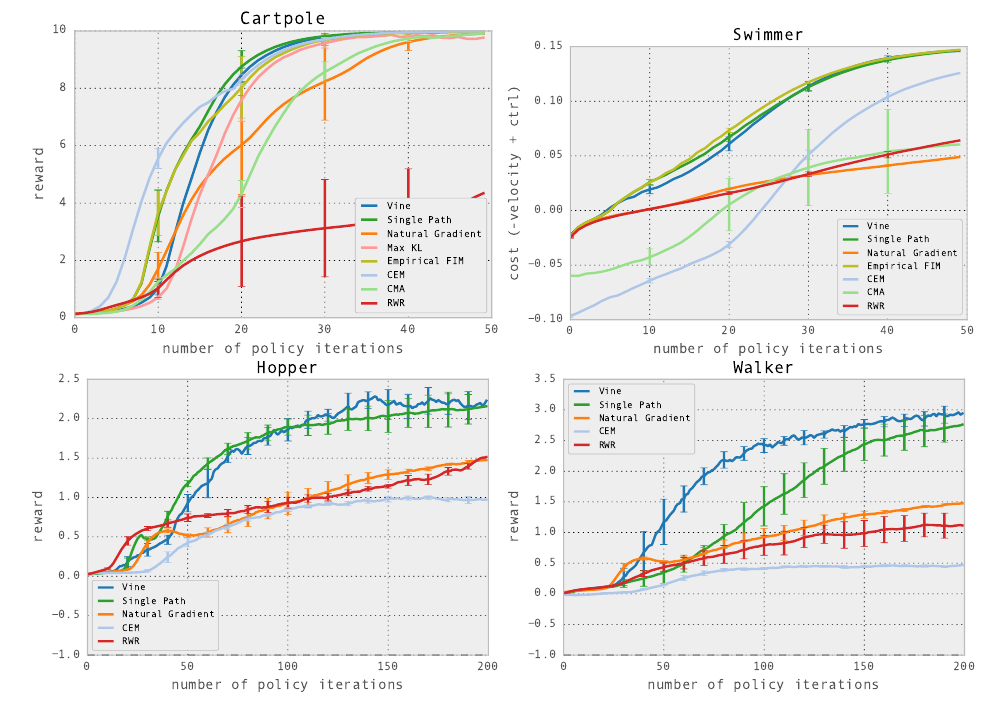
\includegraphics[width=\linewidth, height=0.78\textheight, keepaspectratio]{trpo_fig4_mujoco.png}
%     \end{column}
%     \begin{column}{0.42\textwidth}
%       \small
%       \begin{itemize}
%         \item Swimmer, hopper, walker: torques from joint states; neural-net policies.
%         \item<2-> \textbf{\color{AtlasCool}Vine, single path}: solve all tasks, best scores.
%         \item<3-> \textbf{Natural gradient} (fixed step): no hopping or walking gait.
%         \item<3-> \textbf{CEM, CMA} (derivative-free): poor on the larger networks.
%         \item<4-> \textbf{Max KL} (cart-pole only): a bit slower than mean KL --- the simplification costs little.
%       \end{itemize}
%       \vspace{4pt}
%       \uncover<4->{{\footnotesize Same $\delta=0.01$ in every experiment.}}
%     \end{column}
%   \end{columns}
%   \note{\footnotesize TRPO, Sec.~8.1 and Fig.~4 (cropped from arXiv 1502.05477v5, p.~7). Learning curves averaged over five runs. Hopper and walker: a score of $-1$ is achievable by standing still, so a curve above it means forward progress. Paper: ``constraining the KL divergence is a more robust way to choose step sizes and make fast, consistent progress, compared to using a fixed penalty''; natural gradient used a step size swept in factors of three. Empirical FIM: same as single path but Fisher from the covariance of gradients (cart-pole and swimmer only). Policies use general-purpose networks and simple rewards, no hand-designed gait structure.}
% \end{frame}

% % ---------------- TRPO: Atari ----------------
% \begin{frame}{TRPO: Atari From Raw Pixels}
%   \begin{center}
%   \footnotesize
%   \renewcommand{\arraystretch}{1.2}
%   \setlength{\tabcolsep}{5pt}
%   \begin{tabular}{l r r r r r r r}
%     \toprule
%      & B.\,Rider & Breakout & Enduro & Pong & Q*bert & Seaquest & S.\,Invaders \\
%     \midrule
%     {\color{NoteGray}Random} & {\color{NoteGray}354} & {\color{NoteGray}1.2} & {\color{NoteGray}0} & {\color{NoteGray}$-20.4$} & {\color{NoteGray}157} & {\color{NoteGray}110} & {\color{NoteGray}179} \\
%     {\color{NoteGray}Human} & {\color{NoteGray}7456} & {\color{NoteGray}31.0} & {\color{NoteGray}368} & {\color{NoteGray}$-3.0$} & {\color{NoteGray}18900} & {\color{NoteGray}28010} & {\color{NoteGray}3690} \\
%     Deep Q-learning & 4092 & 168.0 & 470 & 20.0 & 1952 & 1705 & 581 \\
%     UCC-I (MCTS) & 5702 & 380 & 741 & 21 & 20025 & 2995 & 692 \\
%     \midrule
%     \textbf{\color{AtlasCool}TRPO single path} & 1425.2 & 10.8 & \textbf{534.6} & \textbf{20.9} & \textbf{1973.5} & \textbf{1908.6} & 568.4 \\
%     \textbf{\color{AtlasCool}TRPO vine} & 859.5 & 34.2 & 430.8 & \textbf{20.9} & \textbf{7732.5} & 788.4 & 450.2 \\
%     \bottomrule
%   \end{tabular}
%   \end{center}
%   {\scriptsize\color{NoteGray} Bold: TRPO above Deep Q-learning. One run per game (no error bars).\par}
%   \vspace{8pt}
%   \begin{goodbox}
%     \small Not built for games --- yet the \textbf{same} algorithm and settings as for the robots give reasonable scores everywhere.
%   \end{goodbox}
%   \note{\footnotesize TRPO, Sec.~8.2 and Table~1. Policy: CNN with two conv layers (16 channels, stride 2) and one fully connected layer of 20 units, 33{,}500 parameters. 500 iterations took about 30 hours on a 16-core machine. Paper: ``While our method only outperformed the prior methods on some of the games, it consistently achieved reasonable scores. Unlike the prior methods, our approach was not designed specifically for this task.'' UCC-I (Guo et al., 2014) uses Monte Carlo tree search with supervised training. Vine uses a uniform $q$ on Atari.}
% \end{frame}

% % ---------------- GAE results ----------------
% \begin{frame}{GAE: Choosing $\gamma$ and $\lambda$}
%   \begin{columns}[c]
%     \begin{column}{0.6\textwidth}
%       \centering
%       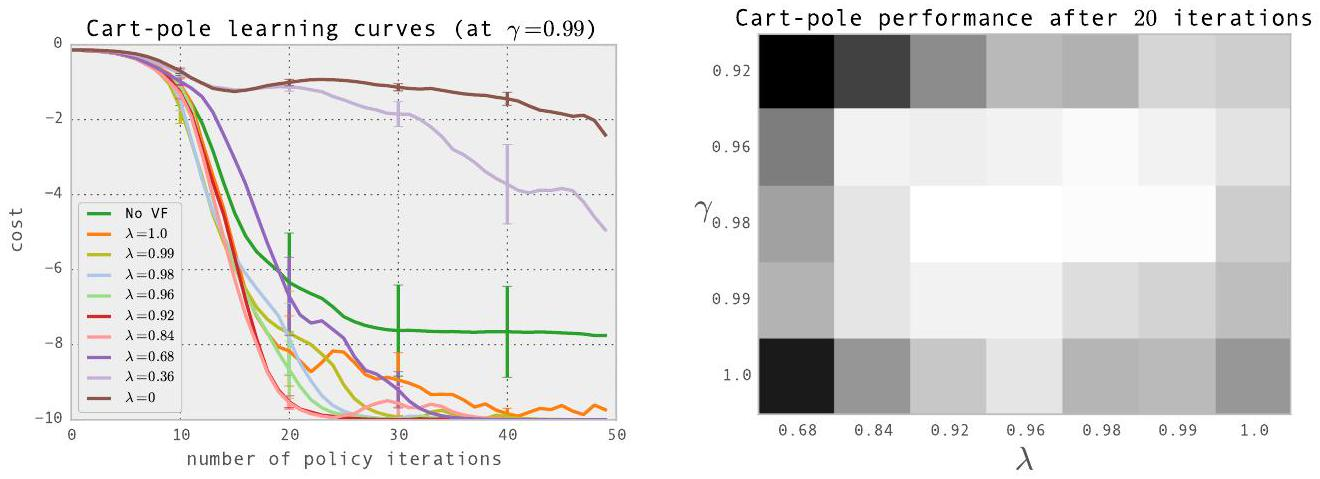
\includegraphics[width=\linewidth, height=0.38\textheight, keepaspectratio]{gae_fig2_sweep.jpg}\par\vspace{4pt}
%       \uncover<2->{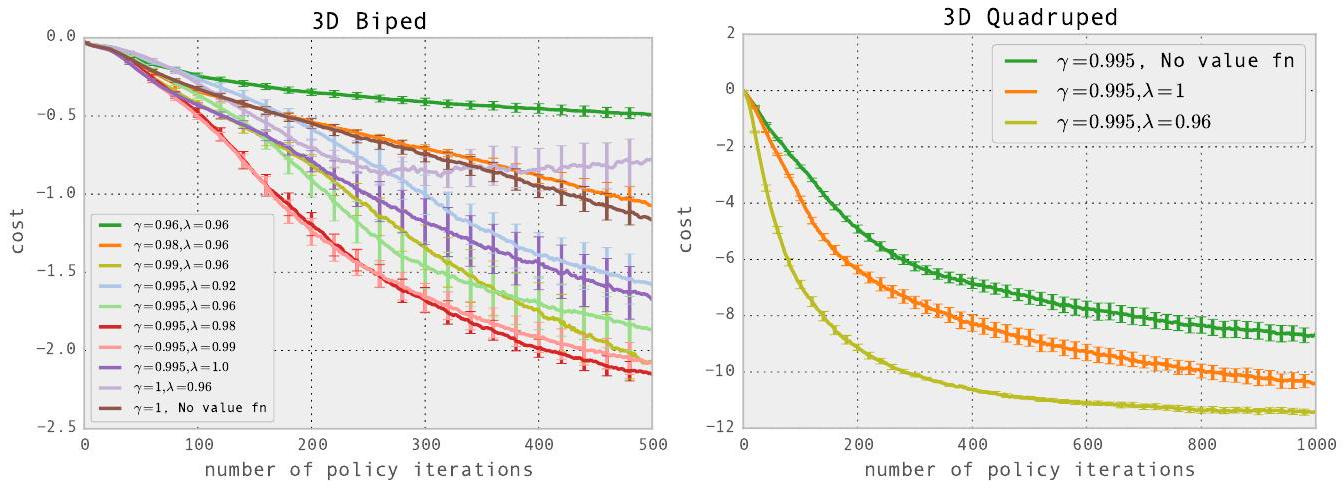
\includegraphics[width=\linewidth, height=0.38\textheight, keepaspectratio]{gae_fig3_3d.jpg}}
%     \end{column}
%     \begin{column}{0.38\textwidth}
%       \small
%       \textbf{Cart-pole} (top; cost, lower is better)
%       \begin{itemize}
%         \item best at intermediate $\lambda\in[0.92,0.99]$
%         \item $\lambda=0$ and ``No VF'' much worse
%       \end{itemize}
%       \uncover<2->{%
%       \textbf{3D biped, quadruped} (bottom)
%       \begin{itemize}
%         \item best $\gamma\in[0.99,0.995]$, $\lambda\in[0.96,0.99]$
%         \item biped runs after 1000 iterations $\approx$ 5.8 days of simulated time
%       \end{itemize}}
%       \uncover<3->{%
%       \begin{slatebox}[top=3pt, bottom=3pt]
%         \small best $\lambda$ $<$ best $\gamma$: $\lambda$ adds bias only if $V$ is wrong.
%       \end{slatebox}}
%     \end{column}
%   \end{columns}
%   \note{\footnotesize GAE, Sec.~6.3, Figs.~2--3 (images from the paper's markdown copy). Plots show cost $=$ negative reward. ``No VF'': a time-dependent baseline (average return at each timestep), no state-value function. Cart-pole: 21 seeds, best $\gamma\in[0.96,0.99]$, $\lambda\in[0.92,0.99]$; right panel: performance after 20 iterations, white $=$ better. Biped: 9 seeds, about 2 hours per trial on a 16-core machine; 5.8 days $=0.01$\,s/step $\times$ 50{,}000 steps/batch $\times$ 1000 batches. Quadruped: $\gamma=0.995$, best with a value function and $\lambda=0.96$. Standing up (Fig.~4, not shown): the value function always helped. Discussion: $\lambda\in[0.9,0.99]$ usually best; App.~A.2: $\lambda=0$ ``prohibitively'' biased.}
% \end{frame}

% % ---------------- Clip vs KL penalty: Table 1 ----------------
% \begin{frame}{Clipping vs.\ KL Penalty: the Ablation}
%   \begin{columns}[c]
%     \begin{column}{0.53\textwidth}
%       \centering
%       \begin{tikzpicture}[x=2.8cm, y=0.36cm, font=\scriptsize]
%         \foreach \y/\lab/\v/\c in {
%             0/No clipping or penalty/-0.39/BadRed!70,
%             1.3/Clipping $\epsilon=0.1$/0.76/AtlasCool!55,
%             2.3/Clipping $\epsilon=0.2$/0.82/AtlasCool,
%             3.3/Clipping $\epsilon=0.3$/0.70/AtlasCool!55,
%             4.6/Adaptive KL $d_{\mathrm{targ}}=0.003$/0.68/AtlasWarm!55,
%             5.6/Adaptive KL $d_{\mathrm{targ}}=0.01$/0.74/AtlasWarm!55,
%             6.6/Adaptive KL $d_{\mathrm{targ}}=0.03$/0.71/AtlasWarm!55,
%             7.9/Fixed KL $\beta=0.3$/0.62/AtlasSlate!40,
%             8.9/Fixed KL $\beta=1$/0.71/AtlasSlate!40,
%             9.9/Fixed KL $\beta=3$/0.72/AtlasSlate!40,
%             10.9/Fixed KL $\beta=10$/0.69/AtlasSlate!40} {
%           \fill[\c] (0,-\y-0.35) rectangle (\v,-\y+0.35);
%           \node[anchor=east] at (-0.42,-\y) {\lab};
%           \node[anchor=west, font=\tiny] at ({max(\v,0)+0.01},-\y) {$\v$};}
%         \draw[gray] (0,0.6) -- (0,-11.5);
%         \node[font=\tiny, NoteGray] at (0,-12.1) {0 = random};
%         \draw[dashed, gray] (1,0.6) -- (1,-11.5);
%         \node[font=\tiny, NoteGray] at (1,-12.1) {1 = best};
%       \end{tikzpicture}
%     \end{column}
%     \begin{column}{0.43\textwidth}
%       \small
%       \textbf{\color{AtlasWarm}Adaptive KL penalty}
%       \begin{gather*}
%         L^{KLPEN} = \hat\E_t\big[r_t\hat A_t - \beta\,\DKL[\pi_{\told},\pi_\theta]\big]
%       \end{gather*}
%       After each update, with $d=\hat\E_t[\DKL]$:
%       \begin{itemize}
%         \item $d < d_{\mathrm{targ}}/1.5$: \ $\beta\leftarrow\beta/2$
%         \item $d > 1.5\,d_{\mathrm{targ}}$: \ $\beta\leftarrow 2\beta$
%       \end{itemize}
%       \vspace{4pt}
%       \begin{coolbox}
%         \small Clipping with $\epsilon=0.2$ wins; the KL penalty stays a useful baseline.
%       \end{coolbox}
%     \end{column}
%   \end{columns}
%   \note{\footnotesize PPO, Sec.~4 and Table~1: 7 MuJoCo tasks, 3 seeds each, 1M timesteps; scores normalized (random $=0$, best $=1$) and averaged over 21 runs. The adaptive rule's constants 1.5 and 2 are heuristic, and the method is not sensitive to them or to the initial $\beta$ (initialized at 1). In concurrent work, Heess et al.\ (2017) used the adaptive-KL variant for 3D locomotion. Clipping in log space was also tried: no better.}
% \end{frame}

% % ---------------- PPO: MuJoCo and Atari ----------------
% \begin{frame}{PPO vs.\ Other Algorithms}
%   \begin{center}
%     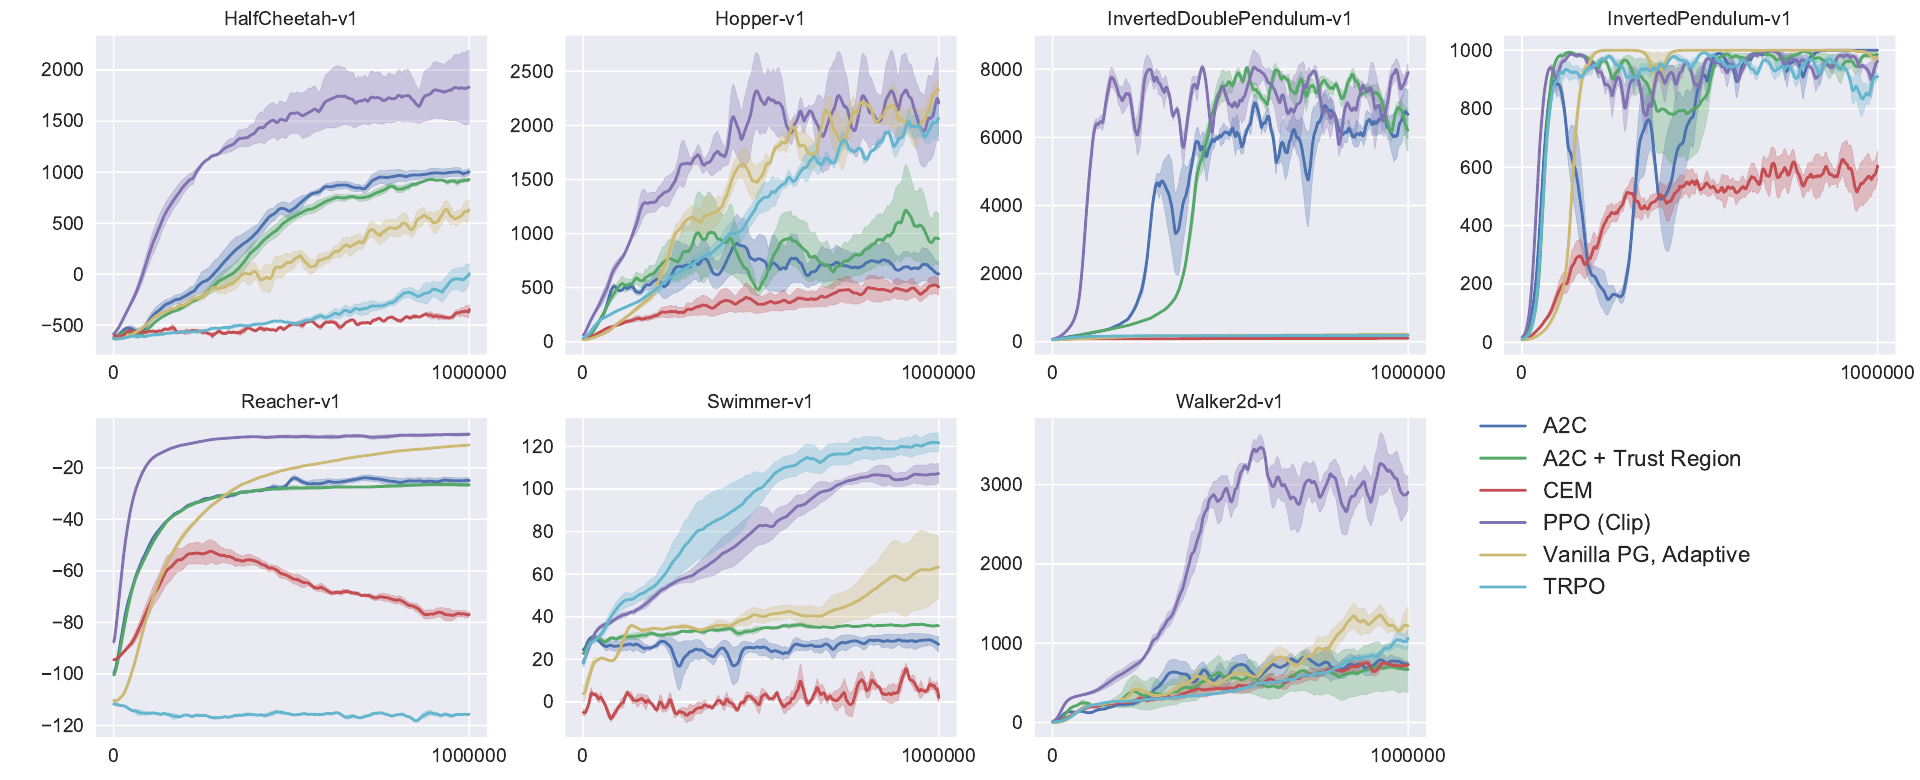
\includegraphics[width=\textwidth, height=0.5\textheight, keepaspectratio]{ppo_fig3_mujoco.png}
%   \end{center}
%   \vspace{-4pt}
%   \begin{columns}[c]
%     \begin{column}{0.5\textwidth}
%       \small
%       \textbf{MuJoCo}, 1M steps: \textbf{\color{AtlasCool}PPO (clip)} best on almost all 7 tasks --- above TRPO, A2C, CEM, vanilla PG.
%     \end{column}
%     \begin{column}{0.46\textwidth}
%       \uncover<2->{%
%       \footnotesize
%       \textbf{Atari}, 49 games --- games won:\par\vspace{2pt}
%       \renewcommand{\arraystretch}{1.1}
%       \setlength{\tabcolsep}{4pt}
%       \begin{tabular}{l r r r}
%         \toprule
%          & A2C & ACER & \textbf{PPO} \\
%         \midrule
%         avg.\ over training & 1 & 18 & \textbf{30} \\
%         last 100 episodes & 1 & \textbf{28} & 19 \\
%         \bottomrule
%       \end{tabular}}
%     \end{column}
%   \end{columns}
%   \note{\footnotesize PPO, Sec.~6.2--6.4, Fig.~3 (cropped from arXiv 1707.06347v2, p.~7) and Table~2. MuJoCo: HalfCheetah, Hopper, InvertedDoublePendulum, InvertedPendulum, Reacher, Swimmer, Walker2d (v1), one million timesteps, tuned baselines; PPO uses $\epsilon=0.2$. Swimmer is the one task where TRPO is clearly ahead. Atari: scoring metric averaged over three trials; ``avg.\ over training'' favors fast learning, ``last 100 episodes'' favors final performance (one tie in the second row). Also in the paper (Sec.~6.3, not shown): 3D humanoid running, steering and getting up (Roboschool).}
% \end{frame}

% ---------------- The whole story ----------------
\begin{frame}{The Whole Story: CPI $\to$ TRPO $\to$ GAE $\to$ PPO}
  \centering
  \begin{tikzpicture}[font=\scriptsize, >=Stealth,
      c/.style={rectangle, rounded corners=2pt, thick,
        text width=2.25cm, align=center, minimum height=0.78cm, inner sep=2pt},
      row/.style={font=\scriptsize\bfseries, anchor=east, align=right, text width=2.2cm}]
    \foreach \x/\h in {0/CPI, 2.75/TRPO, 5.5/GAE, 8.25/PPO}
      \node[font=\small\bfseries, text=AtlasAccent] at (\x,0.75) {\h};
    % lane A: how far
    \node[row, text=AtlasWarm] at (-1.35,0) {A.\ how far may I step?};
    \node[c, cbox=AtlasWarm] (a1) at (0,0) {mixture step $\alpha$};
    \node[c, cbox=AtlasWarm] (a2) at (2.75,0) {KL trust region $\delta$};
    \node[c, cbox=AtlasWarm] (a3) at (5.5,0) {trust region for $\pi$ \textbf{and} $V$};
    \node[c, cbox=AtlasWarm] (a4) at (8.25,0) {clipped ratio $\epsilon$};
    % solver
    \uncover<2->{
    \node[row] at (-1.35,-1.05) {how is it solved?};
    \node[c, cbox=AtlasSlate] (s1) at (0,-1.05) {greedy chooser + formula for $\alpha$};
    \node[c, cbox=AtlasSlate] (s2) at (2.75,-1.05) {CG + line search};
    \node[c, cbox=AtlasSlate] (s3) at (5.5,-1.05) {CG (policy and value)};
    \node[c, cbox=AtlasSlate] (s4) at (8.25,-1.05) {Adam, $K$ epochs};}
    % advantage estimate
    \uncover<3->{
    \node[row] at (-1.35,-2.1) {advantage estimate};
    \node[c, cbox=AtlasSlate] (e1) at (0,-2.1) {rollouts from restarts};
    \node[c, cbox=AtlasSlate] (e2) at (2.75,-2.1) {Monte Carlo $\hat Q$};
    \node[c, cbox=AtlasSlate] (e3) at (5.5,-2.1) {GAE$(\gamma,\lambda)$ + critic};
    \node[c, cbox=AtlasSlate] (e4) at (8.25,-2.1) {truncated GAE};}
    % lane B: where states come from
    \uncover<4->{
    \node[row, text=AtlasCool] at (-1.35,-3.15) {B.\ where do states come from?};
    \node[c, cbox=AtlasCool] (b1) at (0,-3.15) {restarts $s_0\sim\mu$};
    \node[c, draw=BadRed!60, dashed, text=NoteGray] (b2) at (2.75,-3.15) {$\rho_0$ (vine: resets to visited states)};
    \node[c, draw=BadRed!60, dashed, text=NoteGray] (b3) at (5.5,-3.15) {$\rho_0$};
    \node[c, draw=BadRed!60, dashed, text=NoteGray] (b4) at (8.25,-3.15) {$\rho_0$ (+ entropy bonus on actions)};}
    \foreach \i in {1,2,3} \draw[->, AtlasWarm] (a\i) -- (a\the\numexpr\i+1\relax);
    \uncover<2->{\foreach \i in {1,2,3} \draw[->, AtlasSlate] (s\i) -- (s\the\numexpr\i+1\relax);}
    \uncover<3->{\foreach \i in {1,2,3} \draw[->, AtlasSlate] (e\i) -- (e\the\numexpr\i+1\relax);}
    \uncover<4->{\draw[->, BadRed!60, dashed] (b1) -- node[above, font=\tiny, text=BadRed]{dropped} (b2);
      \foreach \i in {2,3} \draw[->, BadRed!40, dashed] (b\i) -- (b\the\numexpr\i+1\relax);}
  \end{tikzpicture}
  \note{\footnotesize Our synthesis. Row A (warm): the same idea at every stage --- keep the new policy close to the one that produced the data, because the surrogate uses the old state distribution. CPI does it by construction, TRPO by a KL constraint, GAE adds a trust region for the critic, PPO by shaping the objective. Row 2: the price of keeping close, from a theoretical step size to an off-the-shelf optimizer. Row 3: from expensive restart rollouts to a learned critic with a bias--variance knob. Row B (cool): CPI's second fix is not carried forward; the only exploration left in TRPO/GAE/PPO is the stochastic policy itself (PPO adds an entropy bonus ``to ensure sufficient exploration'', Sec.~5), which acts on actions, not on start states.}
\end{frame}

% ---------------- One line per paper ----------------
\begin{frame}{One Line per Paper}
  \begin{center}
  \small
  \renewcommand{\arraystretch}{1.45}
  \begin{tabular}{@{}l p{5.2cm} p{5.6cm}@{}}
    \toprule
    \textbf{Paper} & \textbf{Problem it attacks} & \textbf{Main idea} \\
    \midrule
    \textbf{CPI} & greedy updates from approximate values can hurt & conservative mixture, step $\alpha$ from a bound \\
    \textbf{CPI} & on-policy samples miss important states & exploratory restart distribution $\mu$ \\
    \textbf{TRPO} & mixtures don't fit neural-net policies & step size $=$ a policy distance (KL) \\
    \textbf{TRPO} (practice) & the theoretical penalty is far too conservative & mean-KL trust region, CG + line search \\
    \textbf{\color{AtlasWarm}GAE} & $\hat A_t$ from returns is too noisy & critic $V$ + bias--variance knob $\lambda$ \\
    \textbf{\color{AtlasCool}PPO} & second-order step, one step per batch & clipped ratio + minibatch SGD, $K$ epochs \\
    \bottomrule
  \end{tabular}
  \end{center}
  \note{\footnotesize Closing slide; the table follows the story of the talk. Take-home: one idea (stay close to the data-generating policy, measured on its own states) runs from CPI to PPO, made cheaper at each step; the state-coverage idea of CPI was dropped along the way.}
\end{frame}


% ===========================================================================
%  BONUS: PPO for language models -- GRPO (adapted from the Part 1 deck)
% ===========================================================================
\section{Bonus: From PPO to GRPO}

% ---------------- Setting: text generation as RL ----------------
\begin{frame}[label=llm-as-rl]{Text Generation as an RL Problem}
  \centering
  \begin{tikzpicture}[font=\small, >=Stealth,
      tok/.style={rectangle, rounded corners=2pt, draw=AtlasCool, thick, fill=AtlasCool!8,
        minimum width=0.85cm, minimum height=0.6cm, inner sep=1pt}]
    \node[rectangle, rounded corners=2pt, draw=AtlasSlate, thick, fill=AtlasSlate!10,
          minimum height=0.6cm, inner sep=4pt] (x) at (0,0) {question $q\sim P(Q)$};
    \node[tok, right=0.35cm of x] (y1) {$o_1$};
    \node[tok, right=0.25cm of y1] (y2) {$o_2$};
    \node[tok, right=0.25cm of y2] (y3) {$o_3$};
    \node[right=0.2cm of y3] (dots) {$\cdots$};
    \node[tok, right=0.2cm of dots] (eos) {\texttt{EOS}};
    \node[star, star points=5, fill=AtlasWarm, minimum size=0.42cm, inner sep=0pt, right=0.35cm of eos] (r) {};
    \node[right=0.05cm of r, font=\small, AtlasWarm] {$r(q,o)$};
    \draw[decorate, decoration={brace, amplitude=4pt, mirror}, thick, AtlasSlate]
      (x.south west) -- (y2.south east) node[midway, below=5pt, font=\scriptsize, text=AtlasInk]
      {state $s_3=(q,o_{<3})$ \;$\to$\; action $o_3\sim\pi_\theta(\cdot\mid q,o_{<3})$};
    \uncover<2->{
      \draw[decorate, decoration={brace, amplitude=5pt}, thick, AtlasCool]
        (y1.north west) -- (eos.north east) node[midway, above=6pt, font=\scriptsize, text=AtlasCool]
        {bandit view: the whole output $o$ is \textbf{one action}, \ $\pi_\theta(o\mid q)=\prod_t\pi_\theta(o_t\mid q,o_{<t})$};}
  \end{tikzpicture}

  \vspace{10pt}
  \begin{columns}[t]
    \begin{column}{0.32\textwidth}
      \begin{slatebox}[equal height group=llmset]
        \small\raggedright\textbf{Start distribution}\\
        the questions: $q\sim P(Q)$ plays the role of $\rho_0$
      \end{slatebox}
    \end{column}
    \begin{column}{0.32\textwidth}
      \begin{coolbox}[equal height group=llmset]
        \small\raggedright\textbf{\color{AtlasCool}Dynamics}\\
        append the token: \textbf{known} and \textbf{deterministic}
      \end{coolbox}
    \end{column}
    \begin{column}{0.32\textwidth}
      \uncover<3->{%
      \begin{warmbox}[equal height group=llmset]
        \small\raggedright\textbf{\color{AtlasWarm}Reward}\\
        a learned \textbf{reward model} scores $o$ --- only at the end
      \end{warmbox}}
    \end{column}
  \end{columns}
  \note{\footnotesize Token-level MDP as in RLHF with PPO (InstructGPT, Sec.~3.5: ``a bandit environment which presents a random customer prompt and expects a response''; Ahmadian et al.\ 2024, Sec.~2.1: discount 1, reward-model score at \texttt{EOS}). Notation $q,o$ follows DeepSeekMath. The reward model is trained from comparisons (Bradley--Terry, as in InstructGPT); in DeepSeekMath its labels come from checking the final answer. Callback to lane B: known, deterministic dynamics mean that resetting to any prefix is free --- exactly what CPI's restarts $\mu$ and TRPO's vine needed.}
\end{frame}

% ---------------- GRPO: title + setting ----------------
\begin{frame}
  \begin{columns}[c]
    \begin{column}{0.4\textwidth}
      \paperpanel[\large]{DeepSeekMath: Pushing the Limits of Mathematical Reasoning in Open Language Models}
        {Shao, Wang, Zhu, et al.\ (DeepSeek-AI)}{arXiv 2024}
        {Introduces \textbf{GRPO}: PPO without the critic}
    \end{column}
    \begin{column}{0.57\textwidth}
      {\large\bfseries\color{AtlasAccent}Setting \& Assumptions\par}
      \vspace{6pt}
      \small
      \begin{itemize}
        \item Math questions $q$ (GSM8K, MATH; chain of thought), policy: DeepSeekMath-Instruct 7B.
        \item A \textbf{reward model} scores each output $o$ --- at the end (outcome) or per step (process).
        \item Online: $G=64$ outputs per question from the current policy.
        \item Problem with PPO's critic: \textbf{as large as the policy}, and hard to fit per token when the reward comes only at the end.
      \end{itemize}
    \end{column}
  \end{columns}
  \note{\footnotesize DeepSeekMath, Sec.~4.1--4.2. Most of the paper is about pre-training data (120B math tokens from Common Crawl); GRPO is Sec.~4. RL data: about 144K chain-of-thought questions from GSM8K and MATH. KL coefficient 0.04, policy learning rate $10^{-6}$, max length 1024, batch 1024. The reward model is trained on rule-based correctness labels. GRPO later became the RL algorithm of DeepSeek-R1 (2025, not covered). Sec.~4.1.1: ``the value function employed in PPO is typically another model of comparable size as the policy model''.}
\end{frame}

% ---------------- GRPO: group-relative advantages ----------------
\begin{frame}{Group-Relative Advantages}
  \begin{columns}[c]
    \begin{column}{0.5\textwidth}
      \centering
      \begin{tikzpicture}[x=0.75cm, y=2.2cm, >=Stealth]
        \uncover<2->{\fill[AtlasAccent!12] (0.5,0.21) rectangle (6.5,0.79);}
        \node[rectangle, rounded corners=2pt, draw=AtlasSlate, thick, fill=AtlasSlate!10, font=\small] (q) at (3.5,1.55) {question $q$};
        \foreach \i/\r in {1/0.90, 2/0.20, 3/0.70, 4/0.50, 5/0.10, 6/0.60} {
          \draw[->, gray] (q.south) -- (\i,1.1);
          \node[font=\scriptsize] at (\i,1.02) {$o_\i$};
          \ifdim\r pt>0.5pt
            \fill[AtlasCool!70] (\i-0.28,0) rectangle (\i+0.28,\r);
          \else
            \fill[AtlasWarm!70] (\i-0.28,0) rectangle (\i+0.28,\r);
          \fi
          \node[font=\tiny, below] at (\i,0) {$r_\i$};}
        \draw[gray] (0.4,0) -- (6.6,0);
        \draw[AtlasAccent, very thick, dashed] (0.5,0.5) -- (6.5,0.5) node[right, font=\scriptsize]{mean};
        \uncover<2->{\node[right, font=\scriptsize, AtlasAccent] at (6.5,0.79) {$\pm$ std};}
      \end{tikzpicture}
    \end{column}
    \begin{column}{0.48\textwidth}
      \small
      Sample $G$ outputs for the \textbf{same} question; score them.
      \uncover<2->{%
      \begin{formulabox}
        \begin{gather*}
          \hat A_{i,t} = \frac{r_i - \mathrm{mean}(\mathbf r)}{\mathrm{std}(\mathbf r)}
        \end{gather*}
      \end{formulabox}
      {\footnotesize the same value for every token $t$ of $o_i$\par}}
      \uncover<3->{%
        \begin{itemize}
          \item The group mean replaces $V(q)$: a critic computed \textbf{on the fly}.
          \item Matches how RMs are trained: \textbf{comparisons} within one question.
        \end{itemize}}
    \end{column}
  \end{columns}
  \vspace{4pt}
  \uncover<4->{%
  \begin{goodbox}
    \small RL on GSM8K + MATH questions only: GSM8K $82.9\to88.2\%$, MATH $46.8\to51.7\%$, and gains out of domain.
  \end{goodbox}}
  \note{\footnotesize DeepSeekMath, Sec.~4.1.2 (outcome supervision), Table~5. Process supervision (Sec.~4.1.3): normalize the per-step rewards across the group, and give token $t$ the sum of normalized rewards of the steps that end at or after $t$; it did better than outcome supervision (Fig.~5). Out of domain, e.g.\ CMATH $84.6\to88.8\%$. Sec.~5.2.2: RL improves Maj@K but not Pass@K --- it makes the output distribution more robust rather than adding new abilities. Figure: toy rewards, cool $=$ above the mean (pushed up), warm $=$ below (pushed down).}
\end{frame}

% ---------------- GRPO: PPO vs GRPO ----------------
\begin{frame}{PPO vs.\ GRPO}
  \centering
  \begin{tikzpicture}[font=\scriptsize, >=Stealth,
      b/.style={rectangle, rounded corners=2pt, thick,
        minimum height=0.62cm, align=center, inner sep=3pt}]
    % PPO row
    \node[font=\small\bfseries, anchor=east] at (-0.3,0) {PPO};
    \node[b, cbox=AtlasSlate] (q1) at (0.3,0) {$q$};
    \node[b, cbox=AtlasCool] (p1) at (1.8,0) {policy};
    \node[b, cbox=AtlasSlate] (o1) at (3.4,0) {$o$};
    \node[b, cbox=AtlasWarm] (r1) at (5.7,0.75) {reward model};
    \node[b, cbox=AtlasSlate] (f1) at (5.7,0) {reference};
    \node[b, cbox=AtlasWarm, line width=1.4pt] (v1) at (5.7,-0.75) {\textbf{value model}};
    \node[b, cbox=AtlasSlate] (g1) at (8.4,0) {GAE};
    \node[b, cbox=AtlasCool] (a1) at (10.2,0) {$A_t$ per token};
    \draw[->] (q1) -- (p1); \draw[->] (p1) -- (o1);
    \foreach \n in {r1,f1,v1} {\draw[->] (o1.east) -- (\n.west); \draw[->] (\n.east) -- (g1.west);}
    \draw[->] (g1) -- (a1);
    % GRPO row
    \uncover<2->{
    \node[font=\small\bfseries, anchor=east] at (-0.3,-2.2) {GRPO};
    \node[b, cbox=AtlasSlate] (q2) at (0.3,-2.2) {$q$};
    \node[b, cbox=AtlasCool] (p2) at (1.8,-2.2) {policy};
    \node[b, cbox=AtlasSlate] (o2) at (3.4,-2.2) {$o_1,\dots,o_G$};
    \node[b, cbox=AtlasWarm] (r2) at (5.7,-2.2) {reward model};
    \node[b, cbox=AtlasSlate] (g2) at (8.4,-2.2) {group\\ mean, std};
    \node[b, cbox=AtlasCool] (a2) at (10.2,-2.2) {$A_1,\dots,A_G$};
    \node[b, cbox=AtlasSlate] (f2) at (5.7,-3.0) {reference};
    \draw[->] (q2) -- (p2); \draw[->] (p2) -- (o2); \draw[->] (o2) -- (r2);
    \draw[->] (r2) -- node[below]{$r_1..r_G$} (g2); \draw[->] (g2) -- (a2);
    \draw[->, dashed, AtlasSlate] (f2.east) -- (9.3,-3.0) node[right, align=left]{KL goes into\\ the \textbf{loss}};}
  \end{tikzpicture}

  \vspace{6pt}
  \uncover<3->{%
  \begin{formulabox}
    \small
    \begin{gather*}
      \mathcal J_{\mathrm{GRPO}}(\theta) = \E\Big[\frac1G\sum_{i=1}^G\frac{1}{|o_i|}\sum_{t=1}^{|o_i|}
        \Big\{\min\big(\rho_{i,t}\hat A_{i,t},\ \mathrm{clip}(\rho_{i,t},1\pm\varepsilon)\,\hat A_{i,t}\big)
        - \beta\,\DKL\big[\pi_\theta\|\pi_{\mathrm{ref}}\big]\Big\}\Big]
    \end{gather*}
  \end{formulabox}
  {\scriptsize $\rho_{i,t}=\pi_\theta(o_{i,t}|q,o_{i,<t})/\pi_{\told}(o_{i,t}|q,o_{i,<t})$: still PPO's clipped ratio, per token.\par}}
  \note{\footnotesize DeepSeekMath, Sec.~4.1.1, Fig.~4 (redrawn), Eqs.~1--4. PPO for LLMs adds the per-token KL to the reward ($r_t = r_\varphi - \beta\log\pi_\theta/\pi_{\mathrm{ref}}$, following InstructGPT), so the KL passes through GAE; GRPO puts it in the loss instead, which keeps $\hat A$ simple. $\pi_{\mathrm{ref}}$ is usually the initial SFT model. KL estimator (Schulman 2020, ``k3''): $\frac{\pi_{\mathrm{ref}}}{\pi_\theta}-\log\frac{\pi_{\mathrm{ref}}}{\pi_\theta}-1\ge0$, unbiased for $\DKL(\pi_\theta\|\pi_{\mathrm{ref}})$ under samples from $\pi_\theta$. Iterative GRPO (Alg.~1) also retrains the reward model and resets $\pi_{\mathrm{ref}}\leftarrow\pi_\theta$ between rounds.}
\end{frame}

% ---------------- GRPO through the lens of the talk ----------------
\begin{frame}[label=grpo-lens]{GRPO Through the Lens of This Talk}
  \begin{columns}[T]
    \begin{column}{0.48\textwidth}
      \begin{warmbox}[equal height group=grpolens1]
        \small\raggedright\textbf{\color{AtlasWarm}Variance: full circle}\\[2pt]
        GAE learned a critic because Monte Carlo returns were too noisy.
        GRPO goes \textbf{back to Monte Carlo}: $G$ answers per question make a baseline cheap.
      \end{warmbox}
    \end{column}
    \begin{column}{0.48\textwidth}
      \uncover<2->{%
      \begin{coolbox}[equal height group=grpolens1]
        \small\raggedright\textbf{\color{AtlasCool}Two different ``stay close''}\\[2pt]
        clip: near $\pi_{\told}$, so the surrogate stays accurate (as in PPO).\\
        $\beta\,\DKL$: near $\pi_{\mathrm{ref}}$, where the \textbf{reward model} is trusted.
      \end{coolbox}}
    \end{column}
  \end{columns}
  \vspace{6pt}
  \begin{columns}[T]
    \begin{column}{0.48\textwidth}
      \uncover<3->{%
      \begin{slatebox}[equal height group=grpolens2]
        \small\raggedright\textbf{Does the clip ever act?}\\[2pt]
        Their runs: \textbf{one} update per batch $\Rightarrow$ $\pi_\theta=\pi_{\told}$ when the gradient is taken, $\rho_{i,t}=1$.\\
        The clip is idle: REINFORCE + group baseline + KL.
      \end{slatebox}}
    \end{column}
    \begin{column}{0.48\textwidth}
      \uncover<4->{%
      \begin{slatebox}[equal height group=grpolens2]
        \small\raggedright\textbf{RLOO} {\scriptsize(Ahmadian et al.\ 2024)}\\[2pt]
        baseline $b_i$ = mean of the \textbf{other} $G-1$ rewards:
        $r_i-\bar r=\tfrac{G-1}{G}(r_i-b_i)$, the same up to scale.
        Real differences: GRPO's $\mathrm{std}$ and $1/|o_i|$.
      \end{slatebox}}
    \end{column}
  \end{columns}
  \vspace{4pt}
  \uncover<5->{{\centering\footnotesize\textbf{Why the critic could go:} samples per question are cheap, and the question is the only real state.\par}}
  \note{\footnotesize Our synthesis. Box 1: GAE Sec.~1 (variance of Monte Carlo returns) vs.\ DeepSeekMath Sec.~4.1.1 (``uses the average reward of multiple sampled outputs, produced in response to the same question, as the baseline''). Box 2: DeepSeekMath Sec.~4.1.1 adds the KL ``to mitigate over-optimization of the reward model''. Box 3: Sec.~4.2: ``The policy model only has a single update following each exploration stage.'' With $\mu=1$ GRPO iterations, the clip cannot bind; with $\mu>1$ it acts as in PPO. RLOO's paper also reports clipping active on $<5\%$ of each batch in PPO for RLHF (Sec.~3.2). Box 4: RLOO, Sec.~2.3, Eq.~10 (estimator from Kool et al.\ 2019); the algebra $r_i-\frac1G\sum_j r_j=\frac{G-1}{G}\big(r_i-\frac{1}{G-1}\sum_{j\ne i}r_j\big)$ is ours. Dividing by the group std and by $|o_i|$ reweights questions (easy/hard) and answers (short/long); later analyses point at these two terms (Liu et al.\ 2025, ``Understanding R1-Zero-Like Training'', a.k.a.\ Dr.\ GRPO).}
\end{frame}

\begin{frame}{Congratualations ...}

\Huge{You are now a PPO expert !!} 
\vspace{1cm}

\Huge{\hspace{2cm} Let's go and drink some coffee.}

\end{frame}

% ===========================================================================
%  APPENDIX -- optional slides, reached only through links
% ===========================================================================
\appendix

% ---------------- Proof: derivative of eta_mu in alpha (1/3) ----------------
\begin{frame}[label=proof-pa-1]{Proof: $\partial\eta_\mu/\partial\alpha$ at $\alpha=0$ \;(1/3)}
  The conservative mixtures form a \textbf{one-parameter policy class} $\{\pi_\alpha\}_{\alpha\in[0,1]}$:
  \begin{gather*}
    \pi_\alpha(a;s) = (1-\alpha)\,\pi(a;s) + \alpha\,\pi'(a;s)
    \quad\Longrightarrow\quad
    \frac{\partial\pi_\alpha(a;s)}{\partial\alpha} = \pi'(a;s) - \pi(a;s)
  \end{gather*}
  So the policy gradient formula applies as is --- \textbf{$\alpha$ plays the role of $\theta$}:

  \vspace{4pt}
  \centering
  \begin{tikzpicture}[font=\small]
    \node[rectangle, rounded corners=3pt, draw=AtlasCool, line width=0.8pt, fill=AtlasCool!6!white,
          minimum width=11.5cm, align=center, inner sep=4pt] (pg) at (0,0)
      {{\footnotesize\bfseries\color{AtlasCool} Policy gradient, any $\theta\in\mathbb{R}^m$:}\quad
       $\displaystyle \nabla_\theta\,\eta_\mu = \frac{1}{1-\gamma}\sum_s d_{\pi_\theta,\mu}(s)\sum_a \nabla_\theta\pi_\theta(a;s)\,Q_{\pi_\theta}(s,a)$};
    \node[rectangle, rounded corners=3pt, draw=AtlasWarm, line width=0.8pt, fill=AtlasWarm!6!white,
          minimum width=11.5cm, align=center, inner sep=4pt, below=0.75cm of pg] (cp)
      {{\footnotesize\bfseries\color{AtlasWarm} Mixture, at $\alpha=0$ ($\pi_0=\pi$):}\quad
       $\displaystyle \left.\frac{\partial\eta_\mu}{\partial\alpha}\right|_{\alpha=0} = \frac{1}{1-\gamma}\sum_s d_{\pi,\mu}(s)\sum_a \frac{\partial\pi_\alpha(a;s)}{\partial\alpha}\,Q_{\pi}(s,a)$};
    \draw[-{Stealth[length=6pt]}, line width=1pt, draw=AtlasSlate] (pg.south) -- node[right, font=\footnotesize, text=AtlasSlate] {$\theta := \alpha$} (cp.north);
  \end{tikzpicture}

  \vspace{6pt}
  \raggedright
  {\scriptsize\color{NoteGray} The factor $\frac{1}{1-\gamma}$ comes from our normalization: $d_{\pi,\mu}$ sums to 1 and $Q_\pi$ carries a $(1-\gamma)$.}
  \note{\footnotesize Kakade \& Langford, Sec.~4.1, Eq.~4.2 (``straightforward to show \ldots''); the steps are written out here. The key observation: nothing in the policy gradient theorem cares what the parameter means. The mixture weight $\alpha$ is a scalar parameter of the policy class $\{\pi_\alpha\}$, exactly like $\theta$ for $\{\pi_\theta\}$. This is the bridge TRPO builds on (last slide of the proof).}
\end{frame}

% ---------------- Proof: derivative of eta_mu in alpha (2/3) ----------------
\begin{frame}{Proof: $\partial\eta_\mu/\partial\alpha$ at $\alpha=0$ \;(2/3)}
  Substitute the derivative of the mixture:
  \begin{gather*}
    \left.\frac{\partial\eta_\mu}{\partial\alpha}\right|_{\alpha=0}
    = \frac{1}{1-\gamma}\,\E_{s\sim d_{\pi,\mu}}\Big[\sum_a \big(\pi'(a;s)-\pi(a;s)\big)\,Q_\pi(s,a)\Big]
  \end{gather*}
  Since $\sum_a \pi(a;s)\,Q_\pi(s,a) = V_\pi(s)$, $\;\sum_a\pi'(a;s)=1$ and $A_\pi(s,a) = Q_\pi(s,a)-V_\pi(s)$, the inner sum is:
  \begin{gather*}
    \sum_a \pi'(a;s)\,Q_\pi(s,a) - V_\pi(s) = \E_{a\sim\pi'(\cdot;s)}\big[A_\pi(s,a)\big]
  \end{gather*}
  Back into the expectation --- this is the policy advantage $\PA_{\pi,\mu}(\pi')$:
  \begin{formulabox}
    \begin{gather*}
      \left.\frac{\partial\eta_\mu}{\partial\alpha}\right|_{\alpha=0}
      = \frac{1}{1-\gamma}\,\E_{s\sim d_{\pi,\mu}}\Big[\E_{a\sim\pi'(\cdot;s)}\big[A_\pi(s,a)\big]\Big]
      = \frac{1}{1-\gamma}\,\PA_{\pi,\mu}(\pi')
    \end{gather*}
  \end{formulabox}
  \note{\footnotesize Kakade \& Langford, Sec.~4.1. $\square$}
\end{frame}

% ---------------- Proof: why it matters -- alpha and theta (3/3) ----------------
\begin{frame}{Proof: $\alpha$ and $\theta$ Play the Same Role \;(3/3)}
  \centering
  \begin{tikzpicture}[font=\small]
    \node[rectangle, rounded corners=3pt, draw=AtlasWarm, line width=0.8pt, fill=AtlasWarm!6!white,
          text width=5.4cm, align=center, inner sep=6pt, minimum height=3.4cm] (k) at (0,0)
      {{\bfseries\color{AtlasWarm} CPI: parameter $\alpha\in[0,1]$}\\[6pt]
       $\displaystyle\begin{gathered} \eta_\mu(\pi_\alpha) = \eta_\mu(\pi) + \frac{\alpha}{1-\gamma}\,\PA_{\pi,\mu}(\pi') \\ +\, O(\alpha^2) \end{gathered}$\\[6pt]
       {\footnotesize old-state surrogate exact to 1st order\\ (this proof)}\\[4pt]
       {\footnotesize step size:\\ \textbf{$\alpha$ itself}}};
    \node[rectangle, rounded corners=3pt, draw=AtlasCool, line width=0.8pt, fill=AtlasCool!6!white,
          text width=5.4cm, align=center, inner sep=6pt, minimum height=3.4cm] (t) at (7.4,0)
      {{\bfseries\color{AtlasCool} TRPO: parameter $\theta\in\mathbb{R}^m$}\\[6pt]
       $\displaystyle\begin{gathered} \eta(\pi_\theta) = L_{\pi_{\theta_0}}(\pi_\theta) \\ +\, o(\|\theta-\theta_0\|) \end{gathered}$\\[6pt]
       {\footnotesize old-state surrogate exact to 1st order\\ (TRPO Eq.~4)}\\[4pt]
       {\footnotesize step size (Thm.~1):\\ \textbf{$\alpha = D_{\mathrm{TV}}^{\max}(\piold,\pinew)$}}};
    \draw[-{Stealth[length=6pt]}, line width=1pt, draw=AtlasSlate] (k.east) -- node[above, font=\footnotesize, text=AtlasSlate] {generalize} (t.west);
  \end{tikzpicture}

  \vspace{10pt}
  \begin{noteframe}
    \small The proof never used that $\alpha$ is a mixing weight --- only that it parameterizes the policy.
    TRPO keeps the first-order argument for any $\theta$, and replaces ``how far'' ($\alpha$) by a distance between policies.
  \end{noteframe}
  \vfill
  \hfill \hyperlink{policy-advantage}{\beamerreturnbutton{Back to the policy advantage}}-\hyperlink{policy-advantage-recap}{\beamerreturnbutton{Back to the policy advantage recap}}
  \note{\footnotesize Kakade \& Langford, Sec.~4.1; TRPO, Sec.~2--3, Eq.~4 and Thm.~1. TRPO uses unnormalized $\eta$ and $\rho_\pi$, so its constants differ by $(1-\gamma)$ factors. In the mixture, $\alpha$ is both the parameter and the distance: two mixtures differing by $\alpha$ disagree with probability at most $\alpha$. For a general $\pi_\theta$ these are different things, which is why TRPO needs $D_{\mathrm{TV}}$ (then KL).}
\end{frame}

% % ---------------- (2/5) B&T ----------------
% \begin{frame}[label=bt-compare]{Comparing With Bertsekas \& Tsitsiklis (1/5): A Worst Case at Every State}
%   \noindent{\small $\bar A$ as in Lemma 6.1, $\Delta\eta=\eta_\mu(\pi')-\eta_\mu(\pi)$. Given: $\varepsilon=\max_s|\tilde V(s)-V_\pi(s)|$ and $\pi'$ greedy w.r.t.\ $\tilde V$, i.e.\ $T_{\pi'}\tilde V\ge T_\pi\tilde V$,\\
%   where $(T_{\pi'}V)(s)=\E_{a\sim\pi'}\big[(1-\gamma)\mathcal R(s,a)+\gamma\,\E_{s'}V(s')\big]$, so $\bar A = T_{\pi'}V_\pi - V_\pi$.}
%   \begin{gather*}
%     \begin{aligned}
%       T_{\pi'}V_\pi \;&\uncover<2->{\ge\; T_{\pi'}\tilde V - \gamma\varepsilon}
%         && \uncover<2->{\text{\scriptsize\color{NoteGray}$V_\pi$ vs.\ $\tilde V$ at the next state: error $\le\varepsilon$, times $\gamma$}}\\
%       &\uncover<3->{\ge\; T_{\pi}\tilde V - \gamma\varepsilon}
%         && \uncover<3->{\text{\scriptsize\color{NoteGray}$\pi'$ is greedy for $\tilde V$}}\\
%       &\uncover<4->{\ge\; T_\pi V_\pi - 2\gamma\varepsilon \;=\; V_\pi - 2\gamma\varepsilon}
%         && \uncover<4->{\text{\scriptsize\color{NoteGray}the same error again}}
%     \end{aligned}
%   \end{gather*}
%   \uncover<5->{%
%   \begin{warmformulabox}
%     \begin{gather*}
%       \bar A(s) \;\ge\; -2\gamma\varepsilon \ \ \text{at \textbf{every} } s
%       \quad\Longrightarrow\quad
%       \Delta\eta = \frac{1}{1-\gamma}\,\E_{d_{\pi',\mu}}\big[\bar A\big] \;\ge\; -\frac{2\gamma\varepsilon}{1-\gamma}
%     \end{gather*}
%   \end{warmformulabox}}
%   \uncover<6->{%
%   \begin{badbox}
%     \small $\varepsilon$ = \textbf{how wrong our values are}. It only limits how \textbf{negative} $\bar A$ can be;
%     nothing positive is known, since $\pi'$ is greedy for the \emph{wrong} values.
%     {\color{NoteGray}($\varepsilon=0$: $\bar A\ge0$ everywhere --- exact policy improvement.)}
%   \end{badbox}}
%   \note{\footnotesize Our comparison (this and the next four slides), not in the paper. The Gap~1 bound, derived. The two $\varepsilon$'s: once when we replace $V_\pi$ by $\tilde V$ inside $T_{\pi'}$, once when we replace it back inside $T_\pi$; the greedy step in between is the only thing we know about $\pi'$. Each replacement changes a next-state value, hence the factor $\gamma$. Since the bound holds at every state, it holds at whatever states $\pi'$ visits, so we do not need to know $d_{\pi',\mu}$; summing $\sum_t\gamma^t$ gives $\frac{1}{1-\gamma}$. The Gap~1 example shows the per-state bound is reached: $\bar A(s)=-2\gamma\varepsilon$ at the state where $\pi'$ stays.}
% \end{frame}

% % ---------------- (3/5) K&L at alpha=1 ----------------
% \begin{frame}{Comparing With Bertsekas \& Tsitsiklis (2/5): Thm 4.1 at $\alpha=1$}
%   \noindent{\small Split the new states into old states + shift:}
%   \begin{gather*}
%     (1-\gamma)\Delta\eta = \textstyle\sum_s d_{\pi',\mu}(s)\,\bar A(s)
%     \uncover<2->{\;=\; \underbrace{\textstyle\sum_s d_{\pi,\mu}(s)\,\bar A(s)}_{=\,\PA\ \text{(measurable)}}
%       \;+\; \underbrace{\textstyle\sum_s \big(d_{\pi',\mu}-d_{\pi,\mu}\big)(s)\,\bar A(s)}_{\text{shift}}}
%   \end{gather*}
%   \begin{columns}[c]
%     \begin{column}{0.40\textwidth}
%       \centering
%       \begin{tikzpicture}[x=0.8cm, y=0.8cm]
%         \fill[BadRed!14]
%           plot[smooth] coordinates {(0,0.3) (1,0.9) (2,0.7) (3,1.3) (4,0.9) (5,0.3)}
%           -- plot[smooth] coordinates {(5,0.2) (4,0.3) (3,0.5) (2,1.0) (1,1.4) (0,0.3)} -- cycle;
%         \draw[AtlasSlate, very thick] plot[smooth] coordinates {(0,0.3) (1,1.4) (2,1.0) (3,0.5) (4,0.3) (5,0.2)};
%         \draw[AtlasWarm, very thick, dashed] plot[smooth] coordinates {(0,0.3) (1,0.9) (2,0.7) (3,1.3) (4,0.9) (5,0.3)};
%         \draw[->] (0,0) -- (5.4,0) node[right, font=\scriptsize]{$s$};
%         \node[AtlasSlate, font=\scriptsize] at (1.0,1.7) {$d_{\pi,\mu}$};
%         \node[AtlasWarm, font=\scriptsize] at (3.3,1.6) {$d_{\pi',\mu}$};
%       \end{tikzpicture}

%       {\scriptsize \textcolor{BadRed}{shaded}: the shift --- $\bar A$ unknown there.}
%     \end{column}
%     \begin{column}{0.58\textwidth}
%       \small
%       \begin{itemize}
%         \item<3-> Shift $\ge -\|d_{\pi',\mu}-d_{\pi,\mu}\|_1\cdot\varepsilon$, \ with\\
%           $\varepsilon = \max_s|\bar A(s)| = \max_s\big|\E_{a\sim\pi'}A_\pi(s,a)\big|$
%         \item<4-> Same start $\mu$ $\Rightarrow$ only $t\ge1$ can differ:\\
%           $\|d_{\pi',\mu}-d_{\pi,\mu}\|_1 \le (1-\gamma)\sum_{t\ge1}\gamma^t\cdot 2 = 2\gamma$
%       \end{itemize}
%     \end{column}
%   \end{columns}
%   \uncover<5->{%
%   \begin{formulabox}
%     \begin{gather*}
%       \Delta\eta \;\ge\; \frac{\PA}{1-\gamma} - \frac{2\gamma\varepsilon}{1-\gamma}
%       \qquad\text{\small = Thm 4.1 at $\alpha=1$}
%     \end{gather*}
%   \end{formulabox}}
%   \note{\footnotesize Our reading of the proof, at $\alpha=1$. Step 2 adds and subtracts $\sum_s d_{\pi,\mu}(s)\bar A(s)$; the first part is exactly the policy advantage, which rollouts of $\pi$ from $\mu$-restarts can estimate. That is the new ingredient: B\&T never measure any average of the true $\bar A$. Step 3: on the shifted mass we know nothing about the sign of $\bar A$, so we pay its largest size --- this is where Thm 4.1's $\varepsilon$ comes from. It needs $|\cdot|$, not only the negative part, because the shift can also move mass \emph{away} from states where $\bar A>0$, losing part of $\PA$. Step 4: $d=(1-\gamma)\sum_t\gamma^t\Pr(s_t=\cdot)$; at $t=0$ both are $\mu$, for $t\ge1$ the $\ell_1$ distance of two probability distributions is at most $2$. The $2\gamma$ is the same number as in B\&T, from a different place: there, two estimation errors seen one step ahead; here, two state distributions that agree at the start.}
% \end{frame}

% % ---------------- (4/5) general alpha ----------------
% \begin{frame}{Comparing With Bertsekas \& Tsitsiklis (3/5): Why the Mixture Helps}
%   \begin{columns}[c]
%     \begin{column}{0.6\textwidth}
%       \small Same split for $\pinew=(1-\alpha)\pi+\alpha\pi'$:
%       \begin{itemize}
%         \item<1-> Per state: $\bar A_{\mathrm{new}}(s)=\alpha\,\bar A(s)$\\
%           $\Rightarrow$ gain $\alpha\PA$, \ $\max_s|\bar A_{\mathrm{new}}|=\alpha\varepsilon$
%         \item<2-> Shift: $\pinew$ acts like $\pi$ w.p.\ $1-\alpha$ each step,\\
%           $\Pr(\text{deviated by } t)\le 1-(1-\alpha)^t$
%           \begin{gather*}
%             \Rightarrow\ \|d_{\pinew,\mu}-d_{\pi,\mu}\|_1 \le \frac{2\alpha\gamma}{1-\gamma(1-\alpha)}
%           \end{gather*}
%         \item<3-> Multiply: \ $(1-\gamma)\Delta\eta \ge \alpha\PA - \alpha\varepsilon\cdot\dfrac{2\alpha\gamma}{1-\gamma(1-\alpha)}$ \ = Thm 4.1
%       \end{itemize}
%     \end{column}
%     \begin{column}{0.4\textwidth}
%       \centering
%       \uncover<4->{%
%       \gainpenaltyplot

%       {\scriptsize\color{NoteGray} Illustrative: $\gamma=0.6$, $\varepsilon=1$, $\PA=0.6$.}}
%     \end{column}
%   \end{columns}
%   \uncover<5->{%
%   \begin{goodbox}
%     \small Small $\alpha$: the gain wins. \ $\alpha=1$: since $\PA\le\varepsilon$, we need $\PA>2\gamma\varepsilon$ --- impossible for $\gamma\ge\tfrac12$.
%     The positive term alone does not justify the full greedy step; \textbf{the small step does}.
%   \end{goodbox}}
%   \note{\footnotesize Our reading of the proof of Thm 4.1. Gain: $\E_{a\sim\pinew}A_\pi(s,a)=(1-\alpha)\cdot0+\alpha\bar A(s)$, since $\E_{a\sim\pi}A_\pi=0$. Shift: couple the two processes so that they agree until $\pinew$ first picks $\pi'$; then $\|\Pr_t^{\mathrm{new}}-\Pr_t\|_1\le2\big(1-(1-\alpha)^t\big)$ and $(1-\gamma)\sum_t\gamma^t\,2\big(1-(1-\alpha)^t\big)=\frac{2\alpha\gamma}{1-\gamma(1-\alpha)}$. Both factors of the penalty carry an $\alpha$: smaller per-state changes and less shift, hence $\alpha^2$. At $\alpha=1$ the shift factor is $2\gamma$ as on the previous slide. $\PA\le\varepsilon$ because an average of $\bar A$ is at most its maximum. In the plot the green region is where Thm 4.1 guarantees improvement; Cor.~4.2 picks $\alpha$ inside it.}
% \end{frame}

% % ---------------- (5/6) the meaning of epsilon ----------------
% \begin{frame}{Comparing With Bertsekas \& Tsitsiklis (4/5): Same Penalty, Different $\varepsilon$}
%   \begin{center}
%   \renewcommand{\arraystretch}{1.3}
%   \footnotesize
%   \begin{tabular}{l l l l}
%     \toprule
%      & \textbf{\color{AtlasWarm}B\&T} & \textbf{\color{AtlasCool}K\&L, Thm 4.1} & \uncover<2->{\textbf{TRPO, Thm 1}} \\
%     \midrule
%     $\varepsilon=$ & $\max_s|\tilde V(s)-V_\pi(s)|$ & $\max_s|\E_{a\sim\pi'}A_\pi(s,a)|$ & \uncover<2->{$\max_{s,a}|A_\pi(s,a)|$} \\
%     Depends on & our estimate $\tilde V$ & the pair $\pi,\pi'$ & \uncover<2->{$\pi$ only} \\
%     Measures & how wrong our values are & largest one-step gain/loss of $\pi'$ & \uncover<2->{scale of the advantages} \\
%     Step size & fixed: full greedy step & $\alpha$ (mixture weight) & \uncover<2->{$\alpha=\DTV^{\max}(\pi,\tilde\pi)$} \\
%     \bottomrule
%   \end{tabular}
%   \end{center}
%   \begin{itemize}
%     \item<3-> \textbf{Common:} the price of not knowing $\bar A$ on the states the new policy visits.
%     \item<4-> \textbf{Why it changed:} in B\&T, $\pi'$ is fixed by $\tilde V$, so only the estimate can go wrong.
%       K\&L ask a different question --- \emph{how far may we step?} --- so $\varepsilon$ measures the step, not the estimate.
%   \end{itemize}
%   \note{\footnotesize Our synthesis. In both bounds $\varepsilon$ answers the same question: how bad can $\bar A$ be at a state we cannot check? B\&T answer it through the estimate (greedy for values off by $\varepsilon$ $\Rightarrow$ $\bar A\ge-2\gamma\varepsilon$). K\&L answer it through $\pi'$ itself: $|\bar A|\le\varepsilon$ by definition, whatever produced $\pi'$. That is why their $\varepsilon$ depends on $\pi'$: it is not an error but the size of what $\pi'$ changes at a single state. It cannot be estimated either (max over all states), so Cor.~4.2 replaces it by $R$ --- Thm 4.1's $\varepsilon$ is in practice just ``advantages are at most $R$''. The TRPO column is explained on the next slide.}
% \end{frame}

% % ---------------- (6/6) where the error went, and TRPO ----------------
% \begin{frame}{Comparing With Bertsekas \& Tsitsiklis (5/5): Where the Error Went, What TRPO Does}
%   \textbf{Where did B\&T's approximation error go?} Not into Thm 4.1's $\varepsilon$, but into
%   \begin{itemize}
%     \item the estimate of $\PA$ from $\mu$-restarts (sampling error, Hoeffding);
%     \item the accuracy of the greedy chooser $G_\varepsilon$ (CPI slide).
%   \end{itemize}
%   \begin{noteframe}
%     \small Both are \textbf{averages} under $d_{\pi,\mu}$ --- much weaker than B\&T's $\max_s$.
%   \end{noteframe}
%   \vspace{4pt}
%   \uncover<2->{%
%   \textbf{TRPO splits K\&L's $\varepsilon$} into a step and a scale:
%   \begin{formulabox}
%     \begin{gather*}
%       |\bar A(s)| \;\le\; 2\,\underbrace{\DTV\big(\pi(\cdot|s),\tilde\pi(\cdot|s)\big)}_{\text{policy change}\ \le\ \alpha}\cdot\underbrace{\max_{s,a}|A_\pi(s,a)|}_{\text{advantage scale}}
%     \end{gather*}
%   \end{formulabox}}
%   \uncover<3->{%
%   \begin{goodbox}
%     \small The step becomes a \textbf{distance between policies} that the algorithm controls $\Rightarrow$ trust region.
%   \end{goodbox}}
%   \vfill
%   \hfill \hyperlink{improvement-bound}{\beamerreturnbutton{Back to Thm 4.1}}
%   \note{\footnotesize Note the overloaded symbol: the $\varepsilon$ of $G_\varepsilon$ and Thm 4.4 is the chooser's accuracy, not the $\varepsilon$ of Thm 4.1. $G_\varepsilon$ only needs a regression on advantages accurate \emph{on average} under $d_{\pi,\mu}$, unlike B\&T's $\ell_\infty$ requirement. TRPO (App.~A, Lemma~2): couple $a\sim\pi$, $\tilde a\sim\tilde\pi$ to disagree w.p.\ at most $\alpha$; since $\E_{a\sim\pi}A_\pi=0$, $|\bar A(s)|=|\E[A_\pi(s,\tilde a)-A_\pi(s,a)]|\le2\alpha\max|A_\pi|$. So K\&L's $\varepsilon$, which mixed the step and the scale, is factored: the scale $\max|A_\pi|$ depends only on $\pi$, and the step $\alpha$ is a distance between policies. Plugging this into the K\&L argument gives the $4\varepsilon\gamma\alpha^2/(1-\gamma)^2$ penalty, with $4=2\cdot2$.}
% \end{frame}

% ---------------- Backup: d-weighted average = discounted sum over time ----------------
\begin{frame}[label=sum-swap]{From $\E_{s\sim d}$ to a Sum Over Time}
  \begin{columns}[c]
    \begin{column}{0.52\textwidth}
      \small
      \eqstep{1}{\frac{1}{1-\gamma}\E_{s\sim d_{\pi',\mu}}[\bar A(s)] = \frac{1}{1-\gamma}\sum_s d_{\pi',\mu}(s)\,\bar A(s)}
      \vspace{3pt}
      \eqstep{2}{= \sum_s \Big[\sum_t \gamma^t \Pr(s_t{=}s)\Big]\bar A(s)}
      \vspace{3pt}
      \eqstep{3}{= \sum_t \gamma^t \Big[\sum_s \Pr(s_t{=}s)\,\bar A(s)\Big]}
      \vspace{3pt}
      \eqstep{4}{= \sum_t \gamma^t\, \E\big[\bar A(s_t)\big] = \E\Big[\textstyle\sum_t \gamma^t \bar A(s_t)\Big]}
      \vspace{4pt}
      \uncover<5->{\scriptsize
        $\E[\bar A(s_t)]$: over $s_t\sim p_t$, \ $p_t(s)=\Pr(s_t{=}s\mid s_0\sim\mu,\pi')$ --- the state at time $t$, \textbf{not discounted}.\\
        $\E[\sum_t\cdots]$: over trajectories $s_0\sim\mu$, $a_t\sim\pi'(\cdot|s_t)$, $s_{t+1}\sim P(\cdot|s_t,a_t)$.\\
        The discount sits only in the weights $\gamma^t$.\par}
    \end{column}
    \begin{column}{0.46\textwidth}
      \centering
      \uncover<3->{%
      \begin{tikzpicture}[x=0.85cm, y=0.75cm, font=\scriptsize]
        \foreach \t in {0,1,2} \node[AtlasSlate] at (\t,0.8) {$t{=}\t$};
        \node[AtlasSlate] at (3,0.8) {$\cdots$};
        \foreach \s/\y in {1/0,2/-1,3/-2} {
          \node[AtlasWarm] at (-0.75,\y) {$s_\s$};
          \foreach \t in {0,1,2}
            \node[draw=AtlasSlate!40, minimum width=0.75cm, minimum height=0.65cm] at (\t,\y) {};
          \node at (3,\y) {$\cdots$};
          \draw[->, AtlasWarm, thick] (3.35,\y) -- (3.75,\y);
        }
        \node at (1.4,1.45) {cell $(s,t)$: \ $\gamma^t\Pr(s_t{=}s)\,\bar A(s)$};
        \foreach \t in {0,1,2} \draw[->, AtlasSlate, thick] (\t,-2.4) -- (\t,-2.85);
        \node[AtlasWarm, align=left, anchor=west] at (3.8,-1) {row:\\ $\frac{d(s)}{1-\gamma}\bar A(s)$};
        \node[AtlasSlate] at (1,-3.2) {column: $\gamma^t\,\E[\bar A(s_t)]$};
      \end{tikzpicture}

      {\scriptsize Sum the grid by \textcolor{AtlasWarm}{rows} (step 2)\\ or by \textcolor{AtlasSlate}{columns} (step 3): same total.}}
    \end{column}
  \end{columns}
  \vfill
  \hfill \hyperlink{pdl<2>}{\beamerreturnbutton{Back to the lemma}}
  \note{\footnotesize Step 1: an expectation under a distribution on (discrete) states is the weighted sum over states. Step 2: insert the definition $d_{\pi',\mu}(s)=(1-\gamma)\sum_t\gamma^t\Pr(s_t=s;\pi',\mu)$ (Notation slide); the $(1-\gamma)$ cancels, so $d(s)/(1-\gamma)$ is the discounted expected number of visits to $s$. Step 3: the double sum runs over all pairs $(s,t)$; we add the same terms in a different order. This is allowed because every term is bounded in absolute value by $\gamma^t\Pr(s_t=s)R$, and these sum to $R/(1-\gamma)<\infty$ (absolute convergence). Step 4: $\sum_s\Pr(s_t=s)\bar A(s)$ is by definition $\E[\bar A(s_t)]$, the expectation under the time-$t$ state distribution $p_t$ (undiscounted; one distribution per $t$, not a single visitation distribution --- $\sum_t\Pr(s_t=s)$ would not even be normalizable), and linearity moves $\sum_t$ inside the expectation. In the grid, the row of $s$ adds up to its discounted visits times $\bar A(s)$; the column of $t$ adds up to the discounted expected $\bar A$ at time $t$.}
\end{frame}

% ---------------- Gibbs (softmax) policy ----------------
\begin{frame}[label=gibbs-policy]{The Gibbs (Softmax) Policy}
  \begin{columns}[c]
    \begin{column}{0.44\textwidth}
      \centering
      \begin{tikzpicture}[x=0.55cm, y=0.55cm, >=Stealth]
        % left: parameters theta_{sa}
        \node[font=\scriptsize, AtlasSlate] at (1.5,4.3) {scores $\theta_{sa}$};
        \draw[->] (-0.2,0) -- (3.4,0);
        \foreach \x/\h/\a in {0.5/2/a_1, 1.5/1/a_2, 2.5/0.06/a_3}{
          \fill[AtlasSlate!60] (\x-0.35,0) rectangle (\x+0.35,\h*1.6);
          \node[font=\scriptsize, below] at (\x,0) {$\a$};}
        \node[font=\tiny, above] at (0.5,3.2) {2};
        \node[font=\tiny, above] at (1.5,1.6) {1};
        \node[font=\tiny, above] at (2.5,0.1) {0};
        % arrow
        \draw[->, thick, AtlasCool] (3.8,1.6) -- node[above, font=\scriptsize]{softmax} (5.8,1.6);
        % right: probabilities
        \begin{scope}[xshift=3.41cm]
          \node[font=\scriptsize, AtlasCool] at (1.5,4.3) {$\pi_\theta(a;s)$};
          \draw[->] (-0.2,0) -- (3.4,0);
          \foreach \x/\p/\a in {0.5/0.665/a_1, 1.5/0.245/a_2, 2.5/0.090/a_3}{
            \fill[AtlasCool!70] (\x-0.35,0) rectangle (\x+0.35,\p*4.5);
            \node[font=\scriptsize, below] at (\x,0) {$\a$};
            \node[font=\tiny, above] at (\x,\p*4.5) {\p};}
        \end{scope}
      \end{tikzpicture}

      \vspace{4pt}
      {\scriptsize One state $s$, three actions. Every action keeps \textbf{some} probability.}
    \end{column}
    \begin{column}{0.54\textwidth}
      \small One parameter per state--action pair (``table lookup''):
      \begin{coolbox}
        \vspace{-15pt}
        \begin{gather*}
          \pi_\theta(a;s) = \frac{e^{\theta_{sa}}}{\sum_b e^{\theta_{sb}}}
        \end{gather*}
      \end{coolbox}
      \vspace{-2pt}
      \begin{itemize}
        \item \textbf{Why ``Gibbs'':} the Boltzmann distribution of physics, $p \propto e^{-E/T}$, with $\theta = -E/T$.
        \item \textbf{Always stochastic:} $\pi_\theta(a;s) > 0$; deterministic only as $\theta\to\pm\infty$.
        \item \textbf{Rich:} any policy with full support, in every state independently.
        \item \textbf{Simple score:} \\
          $\partial_{\theta_{sb}} \log\pi_\theta(a;s) = \mathbf{1}[a=b] - \pi_\theta(b;s)$
          \hyperlink{gibbs-score}{\beamergotobutton{Derivation}}
      \end{itemize}
    \end{column}
  \end{columns}
  \vfill
  \hfill \hyperlink{pg-reminder<2>}{\beamerreturnbutton{Back to policy gradients}}
  \note{\footnotesize Kakade \& Langford, Sec.~3.2 (Example~2) use ``the common Gibbs table-lookup distributions'' $\{\pi_\theta: \pi(a;s)\propto\exp(\theta_{sa})\}$. Numbers in the figure: $e^2, e^1, e^0$ normalized give $0.665, 0.245, 0.090$. Adding the same constant to all $\theta_{sa}$ of one state leaves $\pi$ unchanged, so the parameters are not unique. A temperature $T$ ($\theta_{sa}/T$) controls how greedy the policy is: $T\to0$ gives argmax, $T\to\infty$ gives uniform. Score: $\nabla\log\pi$ raises the chosen action and lowers all others in proportion to their probability; in REINFORCE it is weighted by the return $\hat Q_t$. The class is rich enough to get arbitrarily close to $\pi^*$, so the trouble in Example~2 comes from the gradient, not from the class. Only parameters of visited states get gradient, which is why a rarely visited state $j$ learns slowly.}
\end{frame}

% ---------------- Gibbs score: derivation ----------------
\begin{frame}[label=gibbs-score]{Deriving the Gibbs Score}
  % Three steps: softmax -> take the log -> differentiate.
  \centering
  \vspace{4pt}
  \eqstep{1}{\pi(a) = \frac{e^{\theta_a}}{\sum_c e^{\theta_c}}}
  \eqsep{2}
  \eqstep{2}{\log\pi(a) = \theta_a - \log\textstyle\sum_c e^{\theta_c}}
  \eqsep{3}
  \eqstep{3}{\partial_{\theta_b}\log\pi(a) = \underbrace{\partial_{\theta_b}\theta_a}_{\mathbf{1}[a=b]} - \underbrace{\frac{e^{\theta_b}}{\sum_c e^{\theta_c}}}_{\pi(b)}}
  \vfill
  \hfill \hyperlink{gibbs-policy}{\beamerreturnbutton{Back to the Gibbs policy}}
  \note{\footnotesize Our derivation. One state $s$, so we drop $s$ from the notation ($\theta_a=\theta_{sa}$). The log turns the fraction into a difference; the first term gives $\mathbf{1}[a=b]$, and by the chain rule the derivative of log-sum-exp is $\frac{e^{\theta_b}}{\sum_c e^{\theta_c}}=\pi(b)$, the softmax itself. Vector form: $\nabla_{\theta_s}\log\pi(a;s) = e_a - \pi(\cdot\,;s)$, ``the action taken minus the average action''. Parameters of other states $s'\neq s$ get derivative $0$ (table lookup). With 2 actions this is the familiar sigmoid result: $\pi(a_1)=\sigma(\theta_1-\theta_2)$ and $(\log\sigma)'=1-\sigma$. Check: $\E_{a\sim\pi}\big[\mathbf{1}[a=b]-\pi(b;s)\big] = 0$, the general identity $\E[\nabla\log\pi]=0$ that makes baselines unbiased. In REINFORCE, taking $a_t$ with $\hat Q_t>0$ raises $\theta_{sa_t}$ by $\alpha\hat Q_t(1-\pi(a_t;s))$ and lowers each other $\theta_{sb}$ by $\alpha\hat Q_t\,\pi(b;s)$.}
\end{frame}

% ---------------- Log-derivative trick: why unbiased ----------------
\begin{frame}[label=log-derivative]{Why the Log-Derivative Trick Is Unbiased}
  \centering
  {\small $\theta$ sits in the \textbf{sampling distribution}, not in $R(\tau)$, so averaging $\nabla_\theta R$ gives nothing.}

  \vspace{4pt}
  \begin{tikzpicture}[st/.style={circle, draw=AtlasSlate, thick, minimum size=0.75cm, font=\small, inner sep=0pt}, >=Stealth]
    \node[font=\small, NoteGray] (D) at (0,0) {$D$};
    \node[st] (s0) at (1.4,0) {$s_0$};
    \node[st] (s1) at (4.6,0) {$s_1$};
    \node[st] (s2) at (7.8,0) {$s_2$};
    \node (dots) at (9.6,0) {$\cdots$};
    \draw[->, thick, NoteGray] (D) -- (s0);
    \foreach \fromnode/\tonode/\idx in {s0/s1/0, s1/s2/1}{
      \draw[->, thick, AtlasSlate] (\fromnode) --
        node[above, font=\scriptsize, text=AtlasCool]{$a_\idx\sim\pi_\theta(\cdot\,;s_\idx)$}
        node[below, font=\scriptsize, text=NoteGray]{$P(\cdot\,;s_\idx,a_\idx)$} (\tonode);}
    \draw[->, thick, AtlasSlate] (s2) -- (dots);
  \end{tikzpicture}

  \vspace{-2pt}
  \begin{gather*}
    p_\theta(\tau) = {\color{NoteGray}D(s_0)}\prod_t {\color{AtlasCool}\pi_\theta(a_t;s_t)}\,{\color{NoteGray}P(s_{t+1};s_t,a_t)}
  \end{gather*}
  \vspace{-6pt}
  \begin{gather*}
    \nabla_\theta\,\eta_D = \sum_\tau \underbrace{\nabla_\theta\, p_\theta(\tau)}_{p_\theta(\tau)\,\nabla_\theta\log p_\theta(\tau)} R(\tau)
      = \E_{\tau\sim\pi_\theta}\big[R(\tau)\,\nabla_\theta\log p_\theta(\tau)\big] \\
    \nabla_\theta\log p_\theta(\tau) = \sum_t \nabla_\theta\log{\color{AtlasCool}\pi_\theta(a_t;s_t)}
      \qquad \text{\scriptsize\color{NoteGray}(log turns $\textstyle\prod$ into $\textstyle\sum$; grey terms have no $\theta$)}
  \end{gather*}

  \vspace{-4pt}
  \begin{coolbox}[width=0.86\linewidth]
    \small $\hat g = R(\tau)\sum_t \nabla_\theta\log\pi_\theta(a_t;s_t)$, \ $\tau\sim\pi_\theta$
    \ $\Rightarrow$ \ $\E[\hat g] = \nabla_\theta\,\eta_D$ \textbf{exactly}, and no need to know $P$.
  \end{coolbox}
  \vfill
  \hfill \hyperlink{pg-sga<3>}{\beamerreturnbutton{Back to PG = SGA}}
  \note{\footnotesize Williams (1992), REINFORCE; also called the score-function or likelihood-ratio estimator. Identity used: $\nabla p = p\,\nabla\log p$ wherever $p>0$. Swapping $\nabla$ and $\sum_\tau$ is fine for a finite horizon (or bounded rewards with discounting); for continuous states or actions, replace sums by integrals. $R(\tau)=(1-\gamma)\sum_t\gamma^t r_t$ as on the PG = SGA slide. Unbiased is not low variance: one rollout gives a very noisy $\hat g$. Two standard changes keep it unbiased: (i) weight each $\nabla\log\pi_\theta(a_t;s_t)$ only by rewards after $t$ (the $\hat Q_t$ of the REINFORCE reminder), since an action cannot affect earlier rewards; (ii) subtract a baseline $b(s_t)$, since $\E_{a\sim\pi_\theta}[\nabla_\theta\log\pi_\theta(a;s)] = \sum_a\nabla_\theta\pi_\theta(a;s) = \nabla_\theta 1 = 0$. With $b=V_\pi$ the weight becomes the advantage, which leads to GAE in PPO. For the Gibbs policy, $\nabla\log\pi$ is the simple score on the Gibbs slide.}
\end{frame}

% ---------------- CPI through the SGD lens ----------------
\begin{frame}[label=cpi-sgd]{CPI Through the SGD Lens}
  \centering
  \vspace{2pt}
  {\small Take the table $\pi(a;s)$ itself as the parameter: CPI is a \textbf{first-order method} on $\eta_\mu$.}

  \vspace{-10pt}
  \footnotesize
  \renewcommand{\arraystretch}{1.3}
  \begin{tabular}{r p{4.3cm} p{6.0cm}}
    & {\color{AtlasSlate}\textbf{SGD (non-convex, smooth)}} & {\color{AtlasWarm}\textbf{CPI}} \\ \hline
    {\color{NoteGray}direction} & $\hat g \approx \nabla J(w)$ & greedy $\pi' = G_\varepsilon(\pi,\mu)$: best linearized direction \\
    {\color{NoteGray}step} & $w \leftarrow w + a_k\,\hat g$ & $\pi \leftarrow (1-\alpha)\,\pi + \alpha\,\pi'$ \quad (Frank--Wolfe step) \\
    {\color{NoteGray}step size} & $\sum_k a_k = \infty$, \ $\sum_k a_k^2 < \infty$ & $\alpha \propto \hat\PA$: slope over a smoothness bound \\
    {\color{NoteGray}noise} & averages out over many steps & each step accurate w.h.p.\ (Hoeffding) \\
    {\color{NoteGray}stationary} & $\|\nabla J(w_R)\| \le \epsilon$, random iterate & $\mathrm{OPT}(\PA_{\pi,\mu}) < 2\varepsilon$, last iterate \\
    {\color{NoteGray}cost} & $O(\sigma^2/\epsilon^4)$ samples & $72R^2/\varepsilon^2$ updates $\times$ $\tilde O(R^2/\varepsilon^2)$ rollouts \\
    {\color{NoteGray}global?} & \xmark\ a stationary point can be bad & \cmark\ Thm.~6.2, up to the mismatch factor \\
  \end{tabular}

  \vspace{4pt}
  \uncover<2->{%
  \begin{coolbox}[width=0.86\linewidth]
    \small Same skeleton: a bounded objective and a sure gain per step $\Rightarrow$ few steps to a stationary point.
    CPI adds Thm.~6.2: \textbf{stationary $\Rightarrow$ near-optimal}.
  \end{coolbox}}
  \vfill
  \hfill \hyperlink{cpi-summary}{\beamerreturnbutton{Back to the three questions}}
  \note<1>{\scriptsize Our synthesis, not in Kakade \& Langford. Notes continue on the next step.
  \textbf{(1) CPI is Frank--Wolfe on the table $\pi(a;s)$.} Policy gradient formula: $\partial\eta_\mu/\partial\pi(a;s) = d_{\pi,\mu}(s)\,Q_\pi(s,a)/(1-\gamma)$. Slope toward $\pi'$: $\langle\nabla\eta_\mu,\pi'-\pi\rangle = \frac{1}{1-\gamma}\sum_s d_{\pi,\mu}(s)\sum_a(\pi'-\pi)(a;s)\,Q_\pi(s,a) = \PA_{\pi,\mu}(\pi')/(1-\gamma)$ (as $\sum_a\pi Q_\pi = V_\pi$), the $\partial\eta_\mu/\partial\alpha$ of the policy advantage slide. So $G_\varepsilon$ maximizes the linearization; per state the maximum is the greedy vertex $\arg\max_a A_\pi(s,a)$. Stepping toward it is Frank--Wolfe (Vieillard, Pietquin \& Geist, 2019, Sec.~3; implicit in Scherrer \& Geist, 2014; Shani et al., 2019). Caveat: $\eta_\mu$ is not concave in $\pi$. $\mathrm{OPT}(\PA)/(1-\gamma)$ is the Frank--Wolfe gap; for smooth non-convex objectives it drops below $\epsilon$ in $O(1/\epsilon^2)$ steps (Lacoste-Julien, 2016), cf.\ $72R^2/\varepsilon^2$.
  \textbf{(2) Gibbs.} $\partial\eta_\mu/\partial\theta_{sa} = d_{\pi,\mu}(s)\,\pi(a;s)\,A_\pi(s,a)/(1-\gamma)$: the same advantage weighted by $d_{\pi,\mu}$, but times $\pi(a;s)$, so good unlikely actions and unvisited states barely move (Ex.~1--2). The natural gradient (Kakade, 2001) drops both factors: $\theta_{sa}\mathrel{+}=\beta A_\pi(s,a)$, i.e.\ $\pi_{\text{new}}\propto\pi\,e^{\beta A_\pi}$, a soft move toward greedy ($\beta\to\infty$: policy iteration). CPI's mixture is the hard version: CPI $\approx$ natural policy gradient on the Gibbs class.}
  \note<2>{\scriptsize \textbf{(3) Link to SGD.} $A_\pi$ and $\PA$ come from $\mu$-restart rollouts, so each step is a noisy first-order step (stochastic Frank--Wolfe). SGD lets unbiased noise cancel over many steps (Robbins--Monro); CPI makes each step accurate to $\pm\varepsilon/3$ w.h.p.\ (Hoeffding, union bound over $\le72R^2/\varepsilon^2$ steps) and steps only if $\hat\PA\ge2\varepsilon/3$: monotone improvement, guarantee for the last iterate. $\alpha=\frac{(1-\gamma)(\hat\PA-\varepsilon/3)}{4R}$ acts like the $1/L$ step: the slope over the curvature behind the $\alpha^2$ penalty of Cor.~4.2. Counting: gain $\ge\varepsilon^2/(72R)$ and $\eta_\mu\le R$, the descent-lemma argument for smooth non-convex GD. Thm.~6.2 is what later theory calls gradient domination (Agarwal, Kakade, Lee \& Mahajan, 2021, with the same mismatch coefficient). Cost row: product of Thm.~4.4's bounds (ours); the paper leaves the cost of $G_\varepsilon$ open (Sec.~7.1).}
\end{frame}

% ---------------- Greedy policy chooser by regression ----------------
\begin{frame}[label=greedy-regression]{Building $G_\varepsilon$ by Regression on Advantages}
\vspace{10pt}
  \centering
  \begin{tikzpicture}[box/.style={draw=AtlasCool, rounded corners=3pt, fill=AtlasCool!8, align=center,
                        font=\scriptsize, minimum height=1.0cm, text width=3.1cm}, >=Stealth]
    \node[box] (data) at (0,0) {\textbf{Data} from $\mu$-restarts\\$s\sim d_{\pi,\mu}$, \ $a$ uniform,\\rollout $\hat Q_\pi(s,a)$};
    \node[box] (fit) at (4.0,0) {\textbf{Regression}\\$f_\pi(s,a)\approx A_\pi(s,a)$};
    \node[box, draw=AtlasWarm, fill=AtlasWarm!10] (pol) at (8.0,0) {\textbf{Greedy in $f_\pi$}\\$\pi'(s)=\arg\max_a f_\pi(s,a)$};
    \draw[->, thick, AtlasSlate] (data) -- (fit);
    \draw[->, thick, AtlasSlate] (fit) -- (pol);
  \end{tikzpicture}

  \vspace{2pt}
  {\small Required accuracy (Sec.~7.1):}
  \vspace{-6pt}
  \begin{gather*}
    L(f_\pi) = \underbrace{\E_{s\sim d_{\pi,\mu}}}_{\text{average over states}}\ \underbrace{\max_a}_{\text{worst action}}\big|A_\pi(s,a)-f_\pi(s,a)\big| \;\le\; \frac{\varepsilon}{2}
  \end{gather*}
  \vspace{-4pt}
  {\small Why it suffices: with $e(s)=\max_a|A_\pi-f_\pi|$, \ $\hat a=\arg\max_a f_\pi$, \ $a^*=\arg\max_a A_\pi$:}
  \vspace{-6pt}
  \begin{gather*}
    A_\pi(s,\hat a) \ge f_\pi(s,\hat a)-e(s) \ge f_\pi(s,a^*)-e(s) \ge A_\pi(s,a^*)-2e(s)\\
    \E_{s\sim d_{\pi,\mu}}\!:\quad \PA_{\pi,\mu}(\pi') \ge \mathrm{OPT}(\PA_{\pi,\mu}) - 2L \ge \mathrm{OPT}(\PA_{\pi,\mu}) - \varepsilon
  \end{gather*}

  \vspace{-4pt}
  \begin{coolbox}[width=0.86\linewidth]
    \small An \textbf{average} ($\ell_1$) error over $d_{\pi,\mu}$, not the $\max_s$ ($\ell_\infty$) error of greedy DP (Eq.~3.1):
    rarely visited states may be fit badly.
  \end{coolbox}
  \vfill
  \hfill \hyperlink{cpi-alg}{\beamerreturnbutton{Back to CPI}}
  \note{\scriptsize Kakade \& Langford, Def.~4.3 and Sec.~7.1; the three-step inequality is ours (the paper calls it ``straightforward''). Here $\PA_{\pi,\mu}(\pi')=\E_{s\sim d_{\pi,\mu}}[A_\pi(s,\hat a)]$ because $\pi'$ is deterministic, and $\mathrm{OPT}(\PA_{\pi,\mu})=\E_{s\sim d_{\pi,\mu}}[\max_a A_\pi(s,a)]$. Data: the same sampling as in Sec.~5 (run from $s_0\sim\mu$, accept each state w.p.\ $1-\gamma$, uniform action, roll out for $\hat Q$). Fitting $Q$ is enough: $A_\pi=Q_\pi-V_\pi(s)$ only shifts each state by a constant, so if $g\approx Q_\pi$ then $f=g-V_\pi$ has the same error against $A_\pi$ and the same $\arg\max$; $V_\pi$ is never needed. Link to usual losses (ours): $\max_a|e|\le\sum_a|e| = n_a\,\E_{a\sim\text{unif}}|e|$, and $\E|e|\le\sqrt{\E e^2}$, so a mean squared error below $(\varepsilon/(2n_a))^2$ under $s\sim d_{\pi,\mu}$, $a$ uniform, is sufficient (pessimistic). The paper does not bound the samples this regression needs, so the total cost of CPI is open; it also notes direct policy search could implement $G_\varepsilon$. Practical descendants: approximate policy iteration with classifiers (Lagoudakis \& Parr, 2003) and Deep CPI.}
\end{frame}

% ---------------- Appendix: geometric stopping samples d ----------------
\begin{frame}[label=geom-stop]{Stopping With Probability $1-\gamma$ Samples $d_{\pi,\mu}$}
  \begin{columns}[c]
    \begin{column}{0.54\textwidth}
      \small
      Run $\pi$ from $s_0\sim\mu$; after each step stop w.p.\ $1-\gamma$, independently of the trajectory. Return $s_\tau$.
      \vspace{4pt}

      \eqstep{1}{\Pr(\tau=t) = \gamma^t(1-\gamma)}
      \vspace{3pt}
      \eqstep{2}{\Pr(s_\tau=s) = \sum_t \Pr(\tau=t)\,\Pr(s_t=s)}
      \vspace{3pt}
      \eqstep{3}{= (1-\gamma)\sum_t \gamma^t\,\Pr(s_t=s\mid\pi,\mu) = d_{\pi,\mu}(s)}
      \vspace{6pt}
      \uncover<4->{\scriptsize
        Step 2 needs independence: $\tau$ does not look at the states.\\
        The $(1-\gamma)$ in $d_{\pi,\mu}$ is what makes $\sum_t\Pr(\tau=t)=1$.\\
        $\gamma$ = probability of surviving one more step; $\E[\tau]=\gamma/(1-\gamma)$.\par}
    \end{column}
    \begin{column}{0.44\textwidth}
      \centering
      \begin{tikzpicture}[x=0.42cm, y=2.4cm, font=\scriptsize]
        \foreach \t in {0,...,9}
          \fill[AtlasCool!70] (\t+0.1,0) rectangle (\t+0.9, {0.3*0.7^\t});
        \draw[->] (0,0) -- (10.6,0) node[right]{$t$};
        \draw[->] (0,0) -- (0,0.42);
        \node[anchor=south west, align=left] at (2.2,0.2) {$\Pr(\tau=t)=(1-\gamma)\gamma^t$\\ ($\gamma=0.7$)};
        \foreach \t in {0,3,6,9} \node[below] at (\t+0.5,0) {$\t$};
      \end{tikzpicture}

      {\scriptsize The discount weights $(1-\gamma)\gamma^t$\\ are a geometric distribution over $t$.}
    \end{column}
  \end{columns}
  \vfill
  \hfill \hyperlink{pa-estimate}{\beamerreturnbutton{Back to estimating $\PA$}}
  \note{\footnotesize Kakade \& Langford, Sec.~5. Step 1: to stop exactly at step $t$ we continue $t$ times (prob.\ $\gamma$ each) and then stop (prob.\ $1-\gamma$), so $\tau$ is geometric. Step 2: total probability over the value of $\tau$; because the stopping coin is independent of the trajectory, $\Pr(\tau=t,\,s_t=s)=\Pr(\tau=t)\Pr(s_t=s)$. Step 3: this is the definition of $d_{\pi,\mu}$ from the Notation slide. So the discount factor can be read as a per-step survival probability, and $d_{\pi,\mu}$ as the distribution of the state where an episode with random length ends. Mean length: $\E[\tau]=\gamma/(1-\gamma)$, about $99$ steps at $\gamma=0.99$, which is the cost of one sample.}
\end{frame}

% ---------------- Appendix: Hoeffding ----------------
\begin{frame}[label=hoeffding]{Hoeffding's Inequality and the Estimate of $\PA$}
  \vspace{8pt}
  \begin{formulabox}
    \begin{gather*}
      \text{If } X_1,\dots,X_k \text{ are \textbf{independent} and } X_i\in[a,b] \text{ a.s., then for } \bar X=\tfrac1k\textstyle\sum_i X_i:\\[2pt]
      \Pr\big(|\bar X-\E\bar X|>\Delta\big) \;\le\; 2\exp\!\Big(-\frac{2k\Delta^2}{(b-a)^2}\Big)
    \end{gather*}
  \end{formulabox}
  \vspace{2pt}
  \uncover<2->{{\small\textbf{Conditions for $x_i$:}}
  \begin{itemize}\small
    \item \textbf{Independent:} each $x_i$ comes from a fresh $\mu$-restart.
    \item \textbf{Bounded:} $\hat Q_i\in[0,R]$, \ $|\pi'-\pi|\le1$ $\Rightarrow$ $x_i\in[-n_aR,\,n_aR]$, \ $b-a=2n_aR$.
    \item \textbf{Right mean:} $\E x_i=\PA$ (uniform $a$, weight $n_a$); bias of a finite rollout kept below $\varepsilon/6$.
  \end{itemize}}
  \uncover<3->{%
  \begin{gather*}
    \Pr\big(|\hat\PA-\PA|>\Delta\big) \;\le\; 2\exp\!\Big(-\frac{2k\Delta^2}{4n_a^2R^2}\Big) = 2e^{-k\Delta^2/(2n_a^2R^2)}\\
    k \;\ge\; \frac{2n_a^2R^2}{\Delta^2}\log\frac2\delta \ \text{ gives error } \le\Delta \text{ w.p.\ } \ge1-\delta
  \end{gather*}}
  \vfill
  \hfill \hyperlink{pa-estimate<3>}{\beamerreturnbutton{Back to estimating $\PA$}}
  \note{\footnotesize Hoeffding (1963). No identical distribution is needed, only independence and a bounded range; no variance enters, so the bound is loose when the $x_i$ rarely reach the ends of the range. The range $2n_aR$ is what costs: the importance weight $n_a$ widens it, hence $k\propto n_a^2$. Sample size: set $2e^{-k\Delta^2/(2n_a^2R^2)}=\delta$ and solve for $k$. In CPI, $\Delta=\varepsilon/3$ and $\delta$ is split over at most $72R^2/\varepsilon^2$ updates (union bound), which gives the $O\big(\frac{R^2}{\varepsilon^2}\log\frac{R^2}{\delta\varepsilon^2}\big)$ restarts per update (the paper drops $n_a$). The rollout bias: $\hat Q_i$ is a truncated return, so $\E x_i$ is within $\varepsilon/6$ of $\PA$ rather than equal; it adds to $\Delta$.}
\end{frame}

% ---------------- Importance sampling (first use: CPI) ----------------
\begin{frame}[label=is-cpi]{Tool: Importance Sampling}
  \noindent{\small The estimate of $\PA$ needs a \textbf{sum} over actions, but each rollout tries \textbf{one} action.}
  \begin{columns}[T]
    \begin{column}{0.52\textwidth}
      \centering\vspace*{6pt}\small
      \eqstep{1}{\text{Sample from $q$, reweight by $w=p/q$} \\ \text{(needs $q>0$ where $p>0$)}\\
        \E_{a\sim p}[f] = \textstyle\sum_a q\,\frac{p}{q}\,f = \E_{a\sim q}\big[w\,f\big]}
      \eqsep{2}
      \eqstep{2}{\text{A plain sum is the case $p\equiv1$; CPI takes $q$ uniform}\\
        \textstyle\sum_a f(a) = \E_{a\sim q}\Big[\frac{f(a)}{q(a)}\Big] = \E_{a\sim\text{unif}}\big[n_a f(a)\big]}
      \eqsep{3}
      \eqstep{3}{\text{Unbiased, but the weight stretches the range}\\
        |f|\le R \;\Rightarrow\; |n_a f|\le n_aR \;\Rightarrow\; n_a^2 \text{ in Hoeffding}}
    \end{column}
    \begin{column}{0.02\textwidth}
      {\color{AtlasSlate!40}\vrule width 0.8pt height 0.62\textheight}
    \end{column}
    \begin{column}{0.42\textwidth}
      \begin{overlayarea}{\linewidth}{0.62\textheight}
      \centering\footnotesize
      \begin{tikzpicture}[x=0.95cm, y=0.55cm]
        \path (-0.6,-1.6) rectangle (4.6,4.2);
        \draw[gray] (-0.4,0) -- (4.4,0);
        % f(a) = 0.6, -0.3, 0.9, 0.2 ; sum = 1.4
        \foreach \i/\f in {1/0.6, 2/-0.3, 3/0.9, 4/0.2} {
          \fill[AtlasCool!70] (\i-0.42,0) rectangle (\i-0.08,\f);
          \node[font=\tiny, below] at (\i,{min(\f,0)}) {$a_{\i}$};}
        \node[AtlasCool, anchor=west] at (-0.5,3.9) {$f(a)$};
        \node[AtlasSlate, anchor=west, font=\tiny] at (-0.5,3.3) {each $a$ drawn w.p.\ $q=1/n_a=\tfrac14$};
        \uncover<2->{
          \foreach \i/\f in {1/2.4, 2/-1.2, 3/3.6, 4/0.8}
            \draw[AtlasWarm, thick] (\i+0.08,0) rectangle (\i+0.42,\f);
          \node[AtlasWarm, anchor=west] at (1.7,3.9) {$n_a f(a)$};
          \draw[AtlasAccent, dashed] (-0.4,1.4) -- (4.4,1.4)
            node[right, font=\tiny, align=left] {mean\\$=\sum_a f$};}
      \end{tikzpicture}\par\vspace{4pt}
      \only<1>{We can evaluate $p$ pointwise, but only draw samples from $q$.}%
      \only<2>{Average of the orange bars under uniform $a$ $=$ sum of the blue bars.}%
      \only<3>{One sampled bar can be $n_a$ times taller $\Rightarrow$ more samples needed. TRPO reuses this with $p=\pi_\theta$, $q=\pi_{\told}$.}
      \end{overlayarea}
    \end{column}
  \end{columns}
  \vfill\hfill\hyperlink{pa-estimate<3>}{\beamerreturnbutton{Back to estimating $\PA$}}
  \note{\footnotesize Introduced here because CPI's estimator (Kakade \& Langford, Sec.~5) already uses it; TRPO and PPO reuse it later (main deck, TRPO part). Identity: for any $q$ with $q(a)>0$ wherever $p(a)f(a)\neq0$, $\E_p[f]=\sum_a p f=\sum_a q\,(p/q)\,f=\E_q[(p/q)f]$. A sum is an ``expectation'' under the weight $p\equiv1$ (counting measure), so $\sum_a f(a)=\E_q[f/q]$; with $q$ uniform the weight is the constant $n_a$ (the number of actions). In CPI, $f(a)=\big(\pi'(a;s)-\pi(a;s)\big)Q_\pi(s,a)$ and $Q_\pi$ is replaced by a rollout estimate $\hat Q_i$, so $x_i=n_a\hat Q_i(s,a)(\pi'-\pi)(a;s)$ has the right mean. Price: the estimate is unbiased for any $q$, but the weight scales the range (and the variance), here from $[-R,R]$ to $[-n_aR,n_aR]$; Hoeffding's bound depends on the squared range, hence $n_a^2$. Figure: four actions, $\sum_a f=1.4$; the weighted values $2.4,-1.2,3.6,0.8$ average to $1.4$. In TRPO the sampling distribution is the old policy and the target the new one, and the trust region keeps the weights near 1 (TRPO's importance sampling slide).}
\end{frame}

% % ---------------- Choice of q in CPI ----------------
% \begin{frame}[label=is-choice]{Why Uniform Actions? Choosing $q$}
%   \noindent{\small At a state $s\sim d_{\pi,\mu}$, the same target can be sampled two ways:}
%   \vspace{-4pt}
%   \begin{gather*}
%     \textstyle\sum_a\big(\pi'-\pi\big)(a;s)\,Q_\pi(s,a)
%     \;=\; \underbrace{\E_{a\sim\text{unif}}\big[n_a(\pi'-\pi)(a;s)\,Q_\pi(s,a)\big]}_{\text{importance sampling, }p\equiv1}
%     \;=\; \underbrace{\E_{a\sim\pi'}\big[Q_\pi(s,a)\big]-V_\pi(s)}_{\text{sample from }\pi'}
%   \end{gather*}
%   \vspace{-6pt}
%   \begin{center}
%   \begin{tikzpicture}[>=Stealth,
%       box/.style={rounded corners=3pt, align=left, font=\scriptsize, text width=5.2cm, inner sep=5pt}]
%     \node[circle, draw=AtlasWarm, fill=AtlasWarm!15, minimum size=7mm, font=\scriptsize] (s) at (0,0) {$s$};
%     \uncover<2->{%
%     \node[box, cbox=AtlasCool, anchor=north east] (u) at (-0.6,-0.5)
%       {\textbf{CPI: $a$ uniform}, one rollout of $\pi$\\
%        $x=n_a(\pi'-\pi)(a;s)\,\hat Q(s,a)\in[-n_aR,\,n_aR]$\\
%        $+$ same data scheme as $G_\varepsilon$ (needs $\hat Q$ for \emph{every} $a$)\\
%        $+$ one batch scores \emph{any} candidate $\pi'$\\
%        $-$ factor $n_a^2$ in the sample count};
%     \draw[->, thick, AtlasCool] (s) -- node[above left, font=\tiny]{$q=1/n_a$} (u.north);}
%     \uncover<3->{%
%     \node[box, cbox=AtlasSlate, anchor=north west] (p) at (0.6,-0.5)
%       {\textbf{Alternative: $a\sim\pi'$}, rollouts of $\pi$\\
%        $x=\hat Q(s,a)-\hat V(s)\in[-R,\,R]$\\
%        $+$ no $n_a$; still only rollouts of $\pi$ (Q2 holds)\\
%        $-$ needs $\pi'$ \emph{before} sampling\\
%        $-$ a second estimate per state ($\hat V$)};
%     \draw[->, thick, AtlasSlate] (s) -- node[above right, font=\tiny]{$q=\pi'$} (p.north);}
%   \end{tikzpicture}
%   \end{center}
%   \vspace{-4pt}
%   \uncover<4->{%
%   \begin{badbox}
%     \small\textbf{Not plain IS with $q=\pi'$:} weight $1/\pi'(a)$, but greedy $\pi'$ is often deterministic, so $\pi'(a)=0$ where $\pi(a)Q_\pi(s,a)\neq0$ and the identity fails.
%   \end{badbox}}
%   \vfill\hfill\hyperlink{pa-estimate<3>}{\beamerreturnbutton{Back to estimating $\PA$}}
%   \note{\footnotesize Our comparison; the paper uses the uniform scheme (Kakade \& Langford, Sec.~5, Eq.~5.1). Why $p\equiv1$: the target is a plain sum over actions; the factor $(\pi'-\pi)$ is signed and does not sum to one, so it is not a distribution and stays inside $f$; every action has weight 1, so $w=1/q=n_a$. Second form: $\sum_a\pi'Q_\pi-\sum_a\pi Q_\pi=\E_{a\sim\pi'}[Q_\pi]-V_\pi(s)$, using $V_\pi=\sum_a\pi Q_\pi$. It is valid and avoids $n_a$: draw $a\sim\pi'$, roll out $\pi$ for $\hat Q$, and estimate $V_\pi(s)$ with a second rollout of $\pi$ from $s$; states still come from $d_{\pi,\mu}$, so no rollouts of $\pi'$ from the start are needed. Why the paper takes uniform actions: step~1 ($G_\varepsilon$) must regress $\hat Q$ for all actions to find the greedy policy, which uniform actions provide, and the same estimator works for any $\pi'$ (including the mixture) without new sampling per candidate. Plain IS with $q=\pi'$ would need $\pi'(a)>0$ wherever $\pi(a)Q_\pi(s,a)\neq0$; a deterministic greedy $\pi'$ violates this. The subtraction of $V_\pi$ in the second form is the same baseline idea that later appears as the advantage in TRPO/PPO.}
% \end{frame}


% ---------------- Continuous spaces: does the theory carry over? ----------------
\begin{frame}[label=trpo-continuous]{Continuous States and Actions?}
  \noindent{\small Back to footnote~1: ``replace the sums with integrals''. \textbf{True} --- no proof uses finiteness.}
  \vspace{4pt}
  \begin{columns}[t]
    \begin{column}{0.45\textwidth}
      {\bfseries\color{AtlasAccent}Why it carries over\par}
      \small
      \begin{itemize}
        \item \textbf{Perf.\ difference}: telescoping, any space.
        \item \textbf{Coupling}: mass $1-\DTV$ on $\{a=\tilde a\}$ --- also for densities.
        \item \textbf{Perturbation} (App.~B): matrices $\to$ Markov operators, same norms.
      \end{itemize}
    \end{column}
    \begin{column}{0.51\textwidth}
      {\bfseries\color{AtlasAccent}What ``integrals'' hides\par}
      \small
      \begin{enumerate}
        \item \textbf{Bounded} $\epsilon = \sup_{s,a}|A_\pi(s,a)| < \infty$.$^{\ast}$
        \item \textbf{max $\to$ sup} over \textbf{all} states, not just visited.
        \item \textbf{Stochastic} policies: deterministic $\Rightarrow \DKL = \infty$.
        \item \textbf{Measurable} kernels; $\rho_\pi$ is a measure.
      \end{enumerate}
    \end{column}
  \end{columns}
  \vfill
  {\color{NoteGray}\rule{0.3\linewidth}{0.4pt}\par}
  {\scriptsize\color{NoteGray}$^{\ast}$\,Often \textbf{vacuous} in continuous control: Gaussian actions with reward $-\|u\|^2$ (their Swimmer) give $\epsilon = \infty$.
  The practical algorithm drops the bound anyway (mean KL, fixed $\delta$).\par}
  \hfill \hyperlink{trpo-thm1}{\beamerreturnbutton{Back to Thm 1}}
  \note{\footnotesize TRPO, footnote~1 (Sec.~3, at the definition of $\DTV$); proofs in App.~A--B. Coupling: the paper cites Levin et al.\ (2009), Prop.~4.7, stated for countable spaces; the maximal coupling, built from $\min(p,q)$, exists on general (standard Borel) spaces and can be chosen measurably in $s$. Perturbation proof: $\|\cdot\|_1$ becomes the total-variation norm on signed measures, $\|\cdot\|_\infty$ the sup norm on functions. Condition 2: the coupling argument needs $\DTV(s)\le\alpha$ at every state either policy can reach, so an essential sup under $\rho_\pi$ is not enough. Condition 4: with deterministic dynamics $\rho_\pi$ can be singular (no density). Swapping $\sum_t$ and $\E$ in Lemma~1 needs the same boundedness as condition~1. Swimmer reward: $r(x,u) = v_x - 10^{-5}\|u\|^2$ (Sec.~8.1). For a Gaussian with fixed $\sigma$: $\DKL(s) = \|\mu_{\mathrm{new}}(s)-\mu_{\mathrm{old}}(s)\|^2/2\sigma^2$.}
\end{frame}

% ---------------- Connections ----------------
\begin{frame}[label=trpo-connections]{One Problem, Several Known Algorithms}
  \begin{center}
  \renewcommand{\arraystretch}{1.3}
  \begin{tabular}{l l l}
    \toprule
    \textbf{Objective} & \textbf{Constraint / penalty} & \textbf{Algorithm} \\
    \midrule
    Linear in $\theta$ & $\tfrac12\|\theta-\told\|^2 \le \delta$ & Vanilla policy gradient \\
    Linear in $\theta$ & Quadratic KL, fixed step $\tfrac{1}{\lambda}$ & Natural policy gradient \\
    Full $L_{\piold}(\pi)$ & none & Policy iteration \\
    $L_{\told}(\theta)$ & $\bar D_{\mathrm{KL}} \le \delta$, enforced & \textbf{TRPO} \\
    \bottomrule
  \end{tabular}
  \end{center}
  \vspace{6pt}
  \begin{itemize}
    \item NPG vs.\ TRPO: same direction $A^{-1}g$; TRPO \textbf{enforces} the KL constraint each step --- matters on larger problems.
    \item Related: REPS constrains the joint $p(s,a)$; TRPO constrains only $\pi(a\mid s)$.
  \end{itemize}
  \vfill
  \hfill \hyperlink{trpo-recap}{\beamerreturnbutton{Back}}
  \note{\footnotesize TRPO, Sec.~7.}
\end{frame}

% ---------------- Appendix: Tool - Importance Sampling ----------------
\begin{frame}[label=is-trpo]{Tool: Importance Sampling}
  % Three steps: identity -> variance -> TRPO. Left: equations. Right: p, q densities + weights.
  \begin{columns}[T]
    \begin{column}{0.67\textwidth}
      \hspace{3pt}
      \centering\vspace*{6pt}\small
      \eqstep{1}{\text{Monte Carlo: an expectation $\approx$ an average of samples}\\
        \E_{a\sim p}[f]\approx\tfrac1n\textstyle\sum_i f(a_i), \quad a_i\sim p\\
        \text{Samples only from $q$? Weight $w = p/q$ ($q>0$ where $p>0$)}\\
        \E_{a\sim p}[f] = \sum_a q\,\frac{p}{q}\,f = \E_{a\sim q}\big[w\,f\big]}
      \eqsep{2}
      \eqstep{2}{\text{Unbiased for any $q$; variance depends on $q$}\\
        \hat\mu = \tfrac1n\textstyle\sum_{i} w(a_i)\,f(a_i), \quad
        \mathrm{Var}[\hat\mu] = \tfrac1n\mathrm{Var}_{q}\big[w f\big]}
      \eqsep{3}
      \eqstep{3}{\text{Policy optimization: estimate expectations under new policy}\\
        p = \pi_\theta(\cdot\mid s), \quad q = \pi_{\told}(\cdot\mid s) \\
        w = \frac{\pi_\theta(a\mid s)}{\pi_{\told}(a\mid s)}}
    \end{column}
    \begin{column}{0.02\textwidth}
      {\color{AtlasSlate!40}\vrule width 0.8pt height 0.66\textheight}
    \end{column}
    \begin{column}{0.5\textwidth}
      \begin{overlayarea}{\linewidth}{0.66\textheight}
      \centering\footnotesize
      \hspace{-40pt}
      \begin{tikzpicture}[x=0.74cm, y=0.88cm]
        % fixed bounding box so the figure does not jump between steps
        \path (-3.1,-2.75) rectangle (3.6,1.95);
        % ---- densities ----
        \draw[gray] (-3,0) -- (3.4,0) node[right] {$a$};
        \draw[AtlasSlate, thick, domain=-3:3.4, samples=80, smooth]
          plot (\x, {3*exp(-(\x)^2/2)/sqrt(2*pi)});
        \node[AtlasSlate, anchor=east] at (-1.1,0.95) {$q$};
        \only<1-2>{
          \draw[AtlasCool, very thick, domain=-0.6:3.4, samples=80, smooth]
            plot (\x, {3*exp(-(\x-1.5)^2/(2*0.49))/(0.7*sqrt(2*pi))});
          \node[AtlasCool] at (2.55,1.55) {$p$};}
        \only<3>{
          \draw[AtlasCool, very thick, domain=-3:3.4, samples=80, smooth]
            plot (\x, {3*exp(-(\x-0.3)^2/2)/sqrt(2*pi)});
          \node[AtlasCool] at (1.6,1.15) {$p$};}
        % samples drawn from q
        \foreach \a in {-1.6,-1.0,-0.5,-0.15,0.2,0.55,0.9,1.3,1.9}
          \fill[AtlasSlate] (\a,0) circle (1.6pt);
        % ---- weights ----
        \uncover<2->{
          \draw[gray] (-3,-2.6) -- (3.4,-2.6);
          \node[anchor=east] at (-2.0,-1.9) {$w = p/q$};
          \draw[AtlasAccent, dashed] (-3,-2.3) -- (3.4,-2.3) node[right, font=\tiny] {$w{=}1$};}
        \only<2>{
          \foreach \a in {-1.6,-1.0,-0.5,-0.15,0.2,0.55,0.9,1.3,1.9} {
            \pgfmathsetmacro{\w}{exp(-(\a-1.5)^2/(2*0.49) + (\a)^2/2)/0.7}
            \fill[AtlasWarm!70] (\a-0.12,-2.6) rectangle (\a+0.12,{-2.6+0.3*\w});}}
        \only<3>{
          \foreach \a in {-1.6,-1.0,-0.5,-0.15,0.2,0.55,0.9,1.3,1.9} {
            \pgfmathsetmacro{\w}{exp(0.3*\a - 0.045)}
            \fill[AtlasCool!60] (\a-0.12,-2.6) rectangle (\a+0.12,{-2.6+0.3*\w});}}
      \end{tikzpicture}\par\vspace{6pt}
      \only<1>{Samples come from $q$, but we want \\ an average under $p$.}%
      \only<2>{$p$ far from $q$: one rare sample carries \\ a huge weight $\Rightarrow$ high variance.}%
      \only<3>{\hspace{-15pt}Trust region keeps $\pi_\theta \approx \pi_{\told}$ $\Rightarrow$ all $w \approx 1$.\\[3pt]
        {\hspace{-15pt}\footnotesize Low variance when $q\approx p$.}}
      \end{overlayarea}
    \end{column}
  \end{columns}

  \vspace{8pt}
  \centering
  \hyperlink{sampling-main}{\beamerreturnbutton{Back to main}}

  \note{\footnotesize
    \textbf{Link to CPI:} CPI's estimate of $\PA$ already used IS with uniform $q$ and weight $n_a$ (appendix); here $q$ is the old policy.
    \textbf{When IS helps:} $p$ can be evaluated pointwise but only samples from $q$ are available. TRPO's case: rollouts come from $\pi_{\told}$, and $\sum_a$ is intractable for continuous actions. Requirement: $\pi_\theta(\cdot\mid s)$ absolutely continuous w.r.t.\ $q(\cdot\mid s)$, so the ratio exists.
    \textbf{Variance:} with $q\approx p$ all weights are near 1 and the variance approaches $\mathrm{Var}_p[f]/n$. A $q$ narrower or lighter-tailed than $p$ is the classic failure: rare, huge weights. So the KL trust region does two jobs: it keeps $L$ accurate and it keeps the weights tame. PPO later clips exactly this ratio.
    \textbf{Why not reweight states too:} that needs $\rho_\theta/\rho_{\told}$, which is unknown. This is why the surrogate keeps $\rho_{\told}$, and why TRPO cannot run offline on a fixed dataset.
    \textbf{Callback to CPI Ex.~1/2:} reweighting whole trajectories gives $w(\tau)=\prod_t \pi(a_t\mid s_t)/\pi_b(a_t\mid s_t)$ (the dynamics cancel), which is exponentially large or small; IS only moves the exponential cost into the variance.
    The vine scheme with continuous actions uses self-normalized IS (next slide).
    Sources: personal notes (statistics, ``Importance sampling''; modern\_rl, TRPO $\to$ Importance sampling); Schervish, \emph{Theory of Statistics}, Sec.~B.7.}
\end{frame}

% ---------------- Appendix: Sampling derivation (1/3) ----------------
\begin{frame}[label=sampling-details-1]{Turning Sums Into Samples: The Problem}
  \textbf{We have:} The local surrogate objective
  \begin{gather*}
    \max_\theta\ L_{\told}(\theta) = \sum_s \rho_{\told}(s) \sum_a \pi_\theta(a\mid s)\, A_{\told}(s,a)
  \end{gather*}

  \vspace{12pt}
  \textbf{The problem:}
  \begin{itemize}
    \item The sum $\sum_s \rho_{\told}(s)[\cdot]$ requires knowing $\rho_{\told}(s)$ for \textbf{all} states
    \item The sum $\sum_a$ requires enumerating all actions
    \item For continuous actions, there is no sum at all
  \end{itemize}

  \vspace{12pt}
  \textbf{What we actually have:}
  \begin{itemize}
    \item States sampled from rollouts: $s \sim \rho_{\told}$
    \item Actions sampled from some policy: $a \sim q$
  \end{itemize}

  \vspace{8pt}
  \begin{noteframe}
    \small Next: transform the sums into expectations we can estimate from samples.
  \end{noteframe}

  \vspace{8pt}
  \centering
  % \hyperlink{sampling-details-2}{\beamerbutton{Next: Step 1}} \quad
  % \hyperlink{sampling-main}{\beamerreturnbutton{Back to main}}

  \note{\footnotesize TRPO, Sec.~5. Setting up the problem: we have a theoretical objective with explicit sums, but in practice we only have samples. The next slides show how to bridge this gap.}
\end{frame}

% ---------------- Appendix: Sampling derivation (2/3) ----------------
\begin{frame}[label=sampling-details-2]{Step 1: From State Sum to Expectation}
  \textbf{Transform the state sum:}
  \begin{gather*}
    \sum_s \rho_{\told}(s)\,[\cdot] = \frac{1}{1-\gamma}\,\E_{s\sim\rho_{\told}}[\cdot]
  \end{gather*}

  \vspace{8pt}
  {\small Since $\rho_{\told}$ is a distribution, the sum equals $(1-\gamma)^{-1}$ times the expectation.}

  \vspace{12pt}
  \textbf{Why this helps:}
  \begin{itemize}
    \item We can estimate expectations by averaging over samples
    \item Just run rollouts under $\pi_{\told}$ and collect states
    \item No need to know $\rho_{\told}(s)$ explicitly
  \end{itemize}

  % \vspace{12pt}
  % \textbf{Also:} Replace advantage with Q-value
  % \begin{gather*}
  %   A_{\told}(s,a) = Q_{\told}(s,a) - V_{\told}(s)
  % \end{gather*}
  % {\small The $V_{\told}(s)$ term doesn't depend on $\theta$, so we drop it \hyperlink{advantage-to-q-explanation}{\beamergotobutton{why?}}}

  \vspace{8pt}
  \centering
  % \hyperlink{sampling-details-3}{\beamerbutton{Next: Step 2}} \quad
  \hyperlink{sampling-main}{\beamerreturnbutton{Back to main}}

  \note{\footnotesize TRPO, Sec.~5, Eq.~13. The factor $(1-\gamma)^{-1}$ is constant in $\theta$ so it can be absorbed into the step size. The $A\to Q$ substitution uses $\sum_a \pi_\theta(a|s) V(s) = V(s)$.}
\end{frame}

% % ---------------- Appendix: Sampling derivation (3/3) ----------------
% \begin{frame}[label=sampling-details-3]{Step 2: From Action Sum to Importance Sampling}
%   \textbf{After Step 1:}
%   \begin{gather*}
%     \max_\theta\ \E_{s\sim\rho_{\told}}\!\left[\sum_a \pi_\theta(a\mid s)\, Q_{\told}(s,a)\right]
%   \end{gather*}

%   \vspace{8pt}
%   \textbf{Remaining issue:} Still have $\sum_a$ over all actions.

%   \vspace{12pt}
%   \textbf{Use importance sampling:}
%   \begin{gather*}
%     \sum_a \pi_\theta(a\mid s)\, Q_{\told}(s,a) = \E_{a\sim q}\!\left[\frac{\pi_\theta(a\mid s)}{q(a\mid s)}\,Q_{\told}(s,a)\right]
%   \end{gather*}

%   {\small Sample actions from any distribution $q$ (e.g., $\pi_{\told}$), then reweight by $\pi_\theta/q$.}

%   \vspace{10pt}
%   \begin{formulabox}
%     \textbf{Final practical objective:}
%     \begin{gather*}
%       \max_\theta\ \E_{s\sim\rho_{\told},\,a\sim q}\!\left[\frac{\pi_\theta(a\mid s)}{q(a\mid s)}\,Q_{\told}(s,a)\right] \\
%       \text{s.t.}\ \ \E_{s\sim\rho_{\told}}\!\big[\DKL(\pi_{\told}(\cdot\mid s)\,\|\,\pi_\theta(\cdot\mid s))\big] \le \delta
%     \end{gather*}
%   \end{formulabox}

%   \vspace{8pt}
%   \centering
%   \hyperlink{sampling-main}{\beamerreturnbutton{Back to main}}

%   \note{\footnotesize TRPO, Sec.~5, Eq.~14. The choice of $q$ (sampling distribution) will be covered in the next slides (single path vs vine). We estimate the expectations by sample averages and $Q$ by Monte Carlo returns.}
% \end{frame}

% ---------------- Appendix: Why A->Q is just a constant ----------------
\begin{frame}[label=advantage-to-q-explanation]{Why Replacing $A$ with $Q$ is Just a Constant Shift}
  \small
  Substitute $A_{\theta_{old}}(s,a) = Q_{\theta_{old}}(s,a) - V_{\theta_{old}}(s)$:
  \begin{gather*}
    \sum_a \pi_\theta(a\mid s) A_{\theta_{old}}(s,a) = \sum_a \pi_\theta(a\mid s) Q_{\theta_{old}}(s,a) - \sum_a \pi_\theta(a\mid s) V_{\theta_{old}}(s)
  \end{gather*}

  \vspace{2pt}
  Since $V_{\theta_{old}}(s)$ doesn't depend on action $a$, pull it out:
  \begin{gather*}
    = \sum_a \pi_\theta(a\mid s) Q_{\theta_{old}}(s,a) - V_{\theta_{old}}(s) \underbrace{\sum_a \pi_\theta(a\mid s)}_{=1}
    = \sum_a \pi_\theta(a\mid s) Q_{\theta_{old}}(s,a) - V_{\theta_{old}}(s)
  \end{gather*}

  \vspace{3pt}
  \textbf{The key:} $V_{\theta_{old}}(s)$ depends on the \textbf{old} policy $\theta_{old}$, \textbf{not} on $\theta$ we're optimizing!
  \begin{gather*}
    \max_\theta [f(\theta) - \text{constant}] = \max_\theta f(\theta)
  \end{gather*}

  \vspace{4pt}
  \centering
  % \hyperlink{sampling-details-2}{\beamerreturnbutton{Back to derivation}} \quad
  \hyperlink{sampling-main}{\beamerreturnbutton{Back to main}}

  \note{\footnotesize The $V$ term is constant with respect to the optimization variable $\theta$, so it doesn't affect which $\theta$ maximizes the objective.}
\end{frame}

\end{document}

